% !Mode: : "TeX: UTF-8"
%%% 本文档可自动生成研究生毕业论文的封面、摘要、目录、正文、参考文献、附录和致谢!等！
\documentclass[acaddeg]{Style/SCNUThesisV3}
%% [2025/3/11   Version 3.0 South China Normal University, Thesis Template, Zhong Liuqiang]
%%% 参数可在acaddeg (学术学位academic degree) 和 profdeg (专业学位 professional degree) 中二选一
%%% 专业学位格式自动满足  华南师范大学教师教育学部 2024 年 11月颁布的华南师范大学研究生学位论文撰写规范！！
%%% 学术学位格式自动满足  华南师范大学数学科学学院 2024 年 11月颁布年颁布的 研究生学位论文撰写规范（适用学科：0701数学）！！
%%% 博士还是硕士, 需要将在 1Cover.tex 中输入.
\usepackage{xeCJK}
\usepackage{Style/scnumacro}
\usepackage{Style/listproc}
\usepackage{Style/ottalt}
\usepackage{textcomp}
\usepackage{graphicx}
\usepackage{quiver}
\setmonofont{Victor Mono}[Scale=.9]
\setCJKfamilyfont{jarm}{Yu Mincho}
\newcommand\ja{\CJKfamily{jarm}\CJKnospace}
\makeatletter
\renewcommand*\verbatim@nolig@list{}
\makeatother

\inputott[rp]{Data/report.ott}
\inputott[dd]{Data/tigrisd}
\renewottcommands[rp]

\input{Style/preamble.tex}

%%%%%%%%%%%%%%%%%%%%%%%%%%%%%%%%%%%%%图表字体和表头设置%%%%%%%%%%%%%%%%%%%%%%%%%%%%%%%%
\usepackage[labelsep=space]{caption}
%%% 自定义的宏包 scnumacro.sty, 已基本包含了所有的数学/表格等环境所需要的宏包

\renewcommand{\baselinestretch}{1.5} % 1.5 倍行距排版
%%图标标题字体设置
\DeclareCaptionFormat{myformat}{\textbf{#1 #2#3}} % #1 是标签，#2 是标题
\captionsetup[figure]{format=myformat} % 应用到figure环境
\captionsetup[table]{format=myformat}
\renewcommand{\baselinestretch}{1.5} % 1.5 倍行距排版
%%%%%%%%%%%%%%%%%%%%%%%%%%%%%%%%%%%%%%%%%%%%%%%%%%%%%%%%%%%%%%%%%%%%%%%%%%%

%\hypersetup{colorlinks=false}%把链接变成红色
\hypersetup{colorlinks=true,
  linkcolor=black,
  filecolor=black,
  urlcolor=black,
citecolor=black,}

\begin{document}
\let\cleardoublepage \clearpage
% 默认每一章应另起一页，每章首页应在奇数页面（右页）, 如果需要去掉空白页, 需要解开上述命令

\newcommand{\clearemptydoublepage}{%
  \clearpage{\pagestyle{empty}\origdoublepage}%
}
\let\origdoublepage\cleardoublepage

%%% ===============================
%%% ======  生成中英文封面  ======
% !Mode:: "TeX:UTF-8"
%%%论文封面
%%  教育硕士专业学位是按   华南师范大学教师教育学部 2024 年 6 月 6 日颁布的华南师范大学研究生学位论文撰写规范  所制定
%%  学术硕士专业学位是按 华南师范大学数学科学学院 2024 年 5 月 23 日颁布年颁布的 研究生学位论文撰写规范（适用学科：0701数学） 所制定

%%%%%%%%%%%%%%%%%%%%%%%%%%%%%%
% 专业学位     中文封面内容
%% “论文分类号”按《中国图书资料分类法》的分类号填写
%%% 具体可查询 http://ztflh.xhma.com
% 分类号 学术型:
% 计算数学 O24   应用数学 O29
% 概率论与数理统计 O21   运筹学  O22
% 统计学 C8   课程与教学论  G427

\classification{}  % 分类号
\UDC{} % UDC: 表示国际十进分类法(Universal Decimal Classification),是世界一般报告或者论文的封面在左上角注明分类号，便于信息交换和处理。
%%%  专业学位的 分类号、UDC：不填写
%%%  学术学位的  分类号: 有  计算数学 O24   应用数学 O29   概率论与数理统计 O21    运筹学  O22 统计学 C8   课程与教学论  G427
\confidential{公开}
%% “密级：学位论文密级分为公开、内部、涉密。内部论文和涉密论文严格按照学校审批的保密级别和保密期限填写，如内部*年、秘密*年；其他论文均填公开
\studentID{20222005253}
%%   填写学位申请人的学号

\type{本~科}

%%% ====================
%%% ====== 中文标题 ======
%%% ====================
%%% 论文标题: 应准确概括整篇论文的核心内容，简明扼要，一般不超过25个汉字。必要时可加副标题。
\title{\CASTunderline[\textwidth]{TinyTheorem：}
  \\ \vspace{0.18cm}
\CASTunderline[\textwidth]{一个依值类型的编程语言暨定理证明器原型}}
%% 如上是封面中的 论文中文标题, 需要人工分行

\titleab{基于依赖类型论的编程语言暨定理证明器实现}
%\subtitle{}    % 中文副标题,  排版时自动居右, 这是可选项, 若不需要可注解掉

%%% ====================
%%% ====== 英文标题 ======
%%% ====================
%%% 英文标题

\etitle{\CASTunderline[\textwidth]{TinyTheorem: }
  \\ \vspace{0.18cm}
  \CASTunderline[\textwidth]{A prototype for a dependently-typed}
  \\ \vspace{0.18cm}
  \CASTunderline[\textwidth]{programming language with theorem proving}
}

%%%==================== ==========
%%%==========  学位申请人 ==========
\author{高振明}
\eauthor{GAO Zhenming}
%%% 英（外）文封面作者姓名按姓在前、名在后的格式书写，姓名需写全拼，如LI Jianguo

%%%==================== ==========
%%%==========  学科专业  ==========
%%% 学科专业: 申请人所在学科专业，必须严格按参照学科代码/专业学位代码字典中的二级学科名称/专业学位领域名称填写，若所选一级学科/专业学位类别下无二级学科/专业学位领域，则填写一级学科/专业学位类别名称，不可用简称。

%%%    学术学位
%  \major{计算数学}
% \emajor{Computional Mathematics}
%  \major{应用数学}
% \emajor{Applied Mathematics}
%  \major{基础数学}
% \emajor{Pure Mathematics}
%  \major{概率论与数理统计}
% \emajor{Probability Theory and Mathematic Statistics}
%  \major{运筹学与控制论}
% \emajor{Operations Research and Cybernetics}

%%%       专业
\major{软件工程}
\emajor{Software Engineering}

%%%==================== ==========
%%%==========   所在学院  ==========
%%% 申请人所在二级培养单位的名称，必须填写与学校官网一致的规范名称，不可用简称。
\college{人工智能学院}
\ecollege{School of Artificial Intelligence}

%%%==================== ==========
%%%==========  导师姓名及职称 ==========
%%%  填写指导教师的姓名与职称。若有两名指导教师，第一（校内）导师姓名和职称写在前面，第二（或校外）导师姓名和职称写在后面，中间空一格。第一（校内）导师必须与研究生管理系统一致。
\advisor{邹竞辉} % 导师姓名
\ProfessionalTitle{讲师} % 及职称
\eadvisor{ZOU Jinhui}  %

%%%==================== ==========
%%%==========  论文完成时间 ==========
% 填写学位论文最终定稿打印成文的年月，封面的日期用汉字书写，如二〇二四年六月、二〇二四年十二月
\submityear{二〇二五} % 年, 用于中文封面
\submitmonth{五}         % 月, 用于中文封面
\submitengyear{2025}  % 年, 用于英文封面
\submitengmonth{MAY} % 月, 用于英文封面
\gradyear{2025}
\gradmonth{7}

\maketitle   % 生成中文封面

\strut\newpage

\begin{cabstract}
  （..略..）
\end{cabstract}

%% 中文关键词, 各关键词之间用逗号隔开, 最后一个关键词不加标点.
%% 关键词一般在3—8个之间.
\begin{ckeywords}
  逻辑推理素养, 高考评价体系, 圆锥曲线, 培养策略
\end{ckeywords}

\begin{center}
  \vskip \stretch{1}
  {
    \begin{spacing}{1.5}
      \songti\bf\erhao {TinyTheorem：}
      \\ \vspace{0.18cm}
      一个依值类型的编程语言暨定理证明器原型
  \end{spacing} } % 论文题目
\end{center}
\vspace{0.68cm}

\makecabstract

\cleardoublepage

\begin{center}
  \vskip \stretch{1}
  {
    \begin{spacing}{1.68}
      \songti\bfseries\erhao
      TinyTheorem:
      \\ \vspace{0.18cm}
      A prototype for a dependently-typed
      \\ \vspace{0.18cm}
      programming language with theorem proving
  \end{spacing} } % 论文题目
  \vspace{0.68cm}
  %\vskip \stretch{1}
\end{center}


\begin{eabstract}
  (..omitted..)
\end{eabstract}

%% 英文关键词, 各关键词之间用逗号隔开. 外文关键词应与中文关键词相对应
\begin{ekeywords}
  logical reasoning literacy, college entrance examination evaluation system, conic curve, cultivation strategies.
\end{ekeywords}
\makeeabstract

%%% ===============================
%%% ======  目   录  ======
%%%      目录
\tableofcontents

%%%  以下内容选用 !!!
%%%% 插图索引
%\listoffigures
%%%% 表格索引
%\listoftables
\newpage\pagenumbering{arabic}\setcounter{page}{1}
%%% 论文正文开始页码编号重新由阿拉伯数字

%%% ===============================
%%% ======  论文的页眉和页脚  ======
\pagestyle{fancy}
\fancyhf{}
\renewcommand{\headrulewidth}{0.8pt}  % 设置横线宽度

\fancyhead[CO]{\wuhao \titleinheader}  % 此处不包含中文封面的副标题, 这里可手工增加中文标题
\fancyhead[CE]{\wuhao 华南师范大学本科毕业论文（设计）}
\cfoot{\thepage}
\fancypagestyle{plain}{
  \pagestyle{fancy}
}
%%% ===========================
%%% ======　论文正文　===========
%%% 在撰写本部分之前, 一定要详细阅读华南师范大学学位论文基本要求
%%%%%% 正文已经默认小四号汉字, 可用如下命令做更改字号 \xiaosihao

\mainmatter

\chapter{绪论}
\section{选题背景及意义}
随着大语言模型、前端框架 React、Vue 的兴起，
作为理论计算机历史悠久的分支之一编程语言理论\&设计实践（Programming Language Theory，PLT \& PL Design \& Implementation, PLDI）与相关领域类型论（Type Theory，TT）、范畴论（Category Theory）重新进入人们的视野。
作为其产物之一的函数式编程范式（functional programming）被活用于前端设计部分，
而另一产物定理证明器则与大模型结合，产生了 AI4MATH 等证明自动化项目。
尝试利用大模型解决奥林匹克数学问题的捷报频传，受到数学家陶哲轩等人的青睐。
然而因其理论程度高（冷门）、对学生纯数学水平要求高的特点，许多大学并未开设该课程，
推广 PLT、PLDI、类型论和范畴论的教育与学界所倡导的编程实践仍然是一项挑战。

本文旨在探索一种同时面向工程化程序开发与形式化验证的语言与编译工具链原型，
同时获得可运行的编译器产出与可用的证明重写器，作为本科生或研究生科研训练与工程原型，
从而成为教学、实验与工程验证的良好平台。
这一原型分为两个子系统（Tigris 语言与 Tigrisd 定理证明器，两者合称 TinyTheorem 解决方案）按序实现：

在程序语言实践层面，本文继承并扩展 Hindley–Milner（HM）类型系统的工程优势（类型推断、简单语义、可扩展的类型类与谓词），通过在工程化实践与更强语言表达力之间进行取舍，创新性地设计出高阶多态、蕴含的谓词约束、严格控制的高阶类型 HKT 构造等语言（类型系统）特性，系统化提升可读、可维护的中型编译器构建能力。产物包括 Tigris 语言、其形式化语言规格（language specifications）和一个可输出多层次结果的编译器、一个基于 IR 的解释器与 REPL。这一子系统使用 Lean 实现；

在形式化验证侧，本文设计了简化的依赖类型（dependent types）内核，
以精简版的依赖类型\lambdacalc（$\lambda$-Calculus）为计算模型，并采用双向（bidirectional）类型检查，
在单一宇宙层级（1-level type theory）下实现蕴含的（impredicative）特性以降低内核复杂度\upcite{norell2007towards,loh2010tutorial}，
用于支持基本的证明对象与重写推理，
产物包括 Tigrisd 语言（定理证明器）、其形式化语言规格和一个可用于定理证明的命令行前端。这一子系统使用 Haskell 实现。

本文借助“解耦”思路，以分离式架构将两个子系统并行推进：编程子系统坚持HM的相对弱的表达力与可编译性；证明子系统把依赖类型的强大表达力局限在更小而可控的内核上，从而避免将全依赖类型的复杂度与代价强加于普通程序员的日常开发环节。
而项目本身，在不牺牲工程实践友好性的前提下，提供一体化但解耦的“语言 + 证明”原型，既便于教学与课程项目落地：如类型推断、闭包转换与续元传递（continuation-passing）化、函数式编程与依赖类型编程实践，
也为进一步研究（如更强的多态、约束求解、编译优化与证明自动化）提供坚实基础与统一框架。

\section{研究现状与文献综述}
以下叙述本项目涉及的研究的现状。为了体现本项目的特殊之处，在每一部分的最后一段，若本文的实现与之有创新，我们加以简要说明。

需要明确的先验认识是：定理证明器也是编程语言，且一般为纯函数式语言，
因为函数式语言在数理逻辑/数学上的合理性（soundness）最好，其中又以纯函数式为甚。
举例来说，数学的函数都没有副作用，这一点在 Haskell 语言中得到体现，除非是
单子上（Monadic，是受范畴论同名代数结构启发，函数式编程中用于建模副作用概念）的函数\footnote{
  而即便是这样的函数，
  除去输入输出、多线程、STM（Software transactional memory）这些真正与副作用相关的 \texttt{IO}、\texttt{ST} Monad 之外，其余都可以用纯函数\emph{模拟}出来，本文的实现亦完全符合这一设计模式，因为 Haskell 和 Lean 都是
  纯函数式语言。
}。
\subsection{Hindley-Milner 类型系统} 由 Hindley、Milner 等奠基并由 Damas–Milner 系统化，形成“具有主类型/类型模式（principal type-schemes）”与“算法W（Algorithm W）”的经典框架\upcite{hindley1969principal,milner1978theory,damas1982principal}。其核心优势为：对 $\lambda$-项的完全/全局类型推断（complete/global type inference）、良好的语义基础与实现简洁性。该系统的后续工作围绕“向多态更强方向扩展”与“保持推断可行性”展开：
\paragraph{类型类（typeclass）与限定类型（qualified types）} 由 Wadler、Blott、Jones 等提出与系统化，提供了对重载与约束多态的统一抽象，使得字典传递成为行之有效的编译期（compile-time）繁饰（elaboration）设计策略\upcite{wadler1989make,jones1993system,jones1995functional}。
\paragraph{高阶多态（higher-rank polymorphism）的推断} 由 Peyton Jones 等提出，Dunfield–Krishnaswami 等人则提供了“完备且易实现的双向类型检查”解决方案，在实践中往往以“显式标注 + 局部推断 + 刚性检查”的折中方式落地\upcite{jones2007practical,dunfield2013complete}。
\paragraph{局部类型推断（local type inference）与双向类型检查} 由 Pierce 提出并发展，则取强表达力与用户心智负担的中间地带：
仅在需要时（例如函数声明，或2-阶及以上时）通过少量标注引导推断，兼顾可读性与可推断性\upcite{dunfield2013complete,pierce2000local}。

\paragraph{本文的创新点} 在本文的“编程子系统”中，我们借鉴上述成果，采用“扩展HM + 谓词（predicates） + 类型类 + 严格一阶类型（strict first-class） + 头等泛型（first-class polymorphism）”的设计，并配以“内嵌一阶模式（Scheme）方案 + Skolem 刚性检查 + 承担字典投影（dictionary projection）的System F繁饰”的实现策略，使其既与 Haskell 传统保持一致性，又便于在原型编译器框架下实现与调试。

\subsection{语法与解析（parsing）} 函数式语言（仅指 Milner 等人开创的 ML 系语言）通常具有相仿
的语法结构。其中著名者包括 Haskell、OCaml、Standard ML；在定理证明器部分则又包括 Coq （现称 Rocq）、Lean、Agda、Isabelle/HOL 与 F*. 函数式语言语法的特点是灵活与统一，
既允许多种多样的用户自定义运算符（例如使用 LR(1) ocamlyacc 实现的 OCaml），更甚者
还支持强大的元编程（metaprogramming）功能，例如 GHC 的 TemplateHaskell，OCaml 的 Pre-Processor Extension （PPX）和 Lean 的 \texttt{syntax}、\texttt{macro}、\texttt{macro\_rules} 等语法构造：
这一特性在定理证明器中尤为明显，因其对数学证明的需求；统一性则体现在函数式语言对语法糖（syntactic sugar）的缺失，得益于这些语言
的面向表达式的特性（expression-oriented），其表层语法（surface syntax）具有强通用性，
且统一使用含类型（typed）\lambdacalc（或其变体，例如定理证明器则使用依赖类型的版本）作为它们的核心代数（core calculus）。从这个角度，也可以说函数式语言\emph{几乎只有}语法糖，因为其表层语法全部被解糖（desugar）到前述的核心代数中，但为了和工业语言特殊对待的“语法糖”区分，我们不称其为语法糖。

\paragraph{本文的创新点} 这些特性，除元编程之外，都由 Tigris 继承。我们设计的表层语法综合了 Lean、OCaml、Haskell 的长处，
并通过受范畴论启发的单子式\footnote{属于函数式编程的设计模式的一部分。}
的语法分析组合子（monadic parser combinator）\upcite{frost1989constructing,Hutton_1992,frost2008parser}
保证解析器的模块化和可维护性，同时利用 Pratt 解析技术实现\upcite{pratt1973top}“用户可定义运算符 + 优先级/结合性”的高可扩展解析能力。
Pratt 自顶向下运算符优先级解析法以其“实现简洁、扩展性强”而被广泛采用，
适合教学与原型构建。结合“分派/分组式 let 语法糖”、
模式匹配（pattern matching）与记录（record）/归纳（代数）数据类型（inductive types/algebraic datatypes）等语言构件，
可覆盖函数式编程主流设计模式。

\subsection{类型类的繁饰与实例解析（instance resolution）} 基于 Wadler-Blott 的类型类思想，
将临时（ad-hoc）多态（例如 C、Java 的函数重载）以“字典”抽象归结为参数化（parametric）多态的系统化繁饰；
Peyton Jones 的合格类型与“构造子类”进一步将类型构造子（如 Functor、Applicative、Monad 等经典纯函数式设计模式\upcite{moggi1991notions}）纳入框架。
在实际实现中，Haskell 主流实现之一的 GHC 的 OutsideIn(X)\upcite{vytiniotis2011outsidein} 体系及其后续演化提出了以约束为中心的求解与实例选择流程，
并辅以 Skolem 刚性变量（rigids）、泛化（generalization）/实例化策略来控制推断过程的完备性与可预测性。

\paragraph{本文的创新点} 本文采用与之相容的思路，但简化了 OutsideIn(X) 体系：
System F 的繁饰以字典参数（项层）+ 类型抽象（类型项层）联合刻画；
刚性检查通过在注解与应用位点进行 Skolem 化检查，防止不当的跨层次统一；
实例解析采用“基于头部匹配 + 递归解析上下文谓词”的策略（参照 OutsideIn 风格），并结合模式匹配决策树优化编译\upcite{maranget2008compiling}。

\subsection{IR 设计与编译后端} 在编译管线方面，
研究社区已就“System F 繁饰 $\to$ Administrative-Normal Form（ANF）$\to$ 闭包转换（closure conversion）$\to$ CPS 化”
的路径形成较为成熟的共识与方法论。这其中，
Girard提出的System F作为多态\lambdacalc 的标准中间表示，适合承载类型抽象与字典化后的多态程序\upcite{reynolds1983types}；
Flanagan、Appel 等人在 ANF 与 CPS 化的经典工作明确了将控制流与求值顺序外显（explicit）化的工程路径\upcite{appel2007compiling,flanagan1993essence}，
利于优化与目标后端对接。

\paragraph{本文的创新点}我们在此基础上，进一步设计了“Lambda IR（ANF 变体）$\to$ CPS IR”的两段式IR，
并最终落地到 Common Lisp\upcite{steele1990common}以获得成熟运行时、交互环境、外部函数接口（foreign function interface，FFI）的支持。

\subsection{依赖类型内核与双向检查} 在证明子系统方面，
Lean、Coq、Agda\upcite{moura2021lean,barras1999coq,bove2009brief}分别代表了现代依赖类型定理证明器的不同取向：
Lean 与 Coq 的理论基础一致（Calculus of Inductive Constructions, CIC）\upcite{coquand1986calculus,Dybjer_1991,10.1007/BF01211308}，但前者强调工程机制与元编程生态，
后者强调严谨公理化\upcite{10.1007/BFb0037116,10.1007/BFb0040259}\footnote{
  前者与后者相比，提供了一些现代逻辑认为不可靠的公理，例如集合论的选择公理（Axiom of Choice），以及由之导出的排中律（Law of Excluded Middle），因而受人诟病；
  而考虑到编程需要，其在停机检查 termination checking 时也较松，允许 partial 和 unsafe. 因而本项目选择用其作为编程语言。
}，
而 Agda 则强调程序化证明与可视化交互，
且主要用于建模（modeling）类型论研究前沿的同伦类型论（Homotopy Type Theory）与立方类型论（Cubical Type Theory）。
而它们的双向检查部分，基本来源于前述编程语言部分类型系统的实现。

\paragraph{本文的创新点}本项目采用“简化依赖类型 + 单一宇宙 + 双向检查”的取舍，参考教学与研究社区中的“pi-forall”、“LambdaPi”等项目经验，
避免把复杂的宇宙层级、多层归纳族与高阶等式推理一次性纳入，实现“可运行、可实验”的证明原型\upcite{loh2010tutorial, brady2005practical}。通过与编程子系统解耦，
用户在不涉及证明时可完全在 HM 子系统内获得流畅的开发体验，
在需要轻量证明与重写时又可切换到依赖类型内核。

\section{主要研究内容、预期目标与创新点}
\subsection{研究的主要内容与设计思路}

在语言前端与解析上，我们将实现 Lean/OCaml/Haskell 风格交融的函数式语法，采用 Pratt 解析构建可扩展的表达式优先级框架，支持用户自定义操作符（优先级/结合性）与冲突检查。表层语法大体依照 OCaml 风格，但参考 Lean 的习惯写法提供语法糖和 Haskell 的写法提供部分语法结构（language construct）与模式匹配、记录/ADT、头等抽象、类型标注（type annotation/ascription）等语法。

在类型系统实现上，构建“扩展 HM + 谓词 + 类型类 + 第一阶 HKT”类型系统；支持 rank-1 方案（TSch）内嵌与字典化繁饰；在语法树（abstract syntax tree, AST）的 \texttt{Ascribe/Var/App} 等关键位点使用 Skolem 刚性检查与rank-1 方案实例（instantiation）；提供局部双向检查与必要的显式标注通道。在类型求解上：采用一阶合一（unification）的方式求解类型、参照“字典变量在作用域内匹配/查找”的 OutsideIn 式思路，维护“已访问实例”集合避免出现环导致系统崩溃（diverge）；在类型制导（type-directed）语法上，我们令类型检查器（typechecker）在需要时（譬如实例解析、解糖时的易歧义处）要求显式类型注解，提升错误定位与歧义时的可预期性。
在IR降级上，我们繁饰表层语法到 System F：新增 Proj（字典投影）等节点便于优化与降级；将类型抽象与字典参数显式化，提供\texttt{TyLam/TyApp/Proj}等 System F IR 结点，并配套$\beta/\eta$-化、减少生成的 IR 噪声并向后续步骤暴露更多的优化机会，同时保证后续变换的可维护性；

在后端 IR 与编译上，我们的管线是 Lambda IR $\to$ Closure Conversion $\to$ CPS Transformation $\to$ Common Lisp；在IR层实现常量折叠（constant folding）、拷贝传播（copy propagation）、无用代码消除（dead code elimination）、尾调用（tailcall/tail-recursive）化、投影/选择消去的源优化，最后在CPS层显式表达控制转移并直接下降到目标 Common Lisp 代码。
模式匹配检查与编译上：在类型全数推断出来后，我们参照 Maranget 的模式匹配冗余/欠缺检查算法，针对缺少的/多余的模式分支向用户发出警告，并针对具体情况向用户提出一种缺失的分支/立即删除多余分支；在System F 繁饰之后，我们根据其基于决策树的编译算法，生成良好分支。

在证明内核部分，我们采用单一宇宙、蕴含式的依赖类型\lambdacalc，并采用双向类型检查，降低判定复杂度与术语成本；
参考标准的等式重写与项代换理论（Baader\&Nipkow）\upcite{baader1998term}提供项重写式（term-rewriting）解释器以支持基本等式推理与程序化证明脚本；利用 Haskell 在学术上的丰富生态，通过 Unbound 等库实现对于\lambdaterm 的操作，变换，以及变量约束的判断；
引入 Peyton Jones 提出的 Weak Head 范式（Weak Head Normal Form, WHNF）\upcite{peyton1987implementation}用于控制消去（reduction），将其与定义性等号（definitional equality）的实现结合，避免在判断两个项是否相等时的无用计算、消去、展开（unfolding），提升定理证明性能。

最后，在实验与评测上，我们以 Functor/Applicative/Monad 等典型代数结构暨函数式编程设计模式为样例，验证实例解析、字典化与投影优化的正确性；以典型函数式程序映射（map）、折叠（fold）考察编译后端的性能与优化效果；
以基本逻辑定理、数学结构的编码作为证明例子，验证证明内核的可用性。

课题整体采用“自顶向下的最小可用（MVP）+ 逐步精炼”的策略。首先保证语言前端、类型系统核心路径、编译与运行链路闭环（从 Tigris 源到 Common Lisp 目标可运行），再迭代增强类型系统细节、实例解析策略与 IR 优化规则。编程与证明两子系统以统一仓库并行推进，但保持边界清晰、依赖方向单纯：编程侧产物可独立使用，
证明侧可以通过两系统相似的表层语法无痛迁移。

\subsection{研究的预期目标}
本课题包含三个目标（要注意，这是最低限度的目标，实际上我们实现的功能并不止与此，见正文）：
{\setlength{\parskip}{-1em}
  \paragraph{其一} 一个可运行的原型编译器与解释器：可编译到 Common Lisp（SBCL）或直接在 REPL 交互下运行；可对带类型类与 HKT 的示例进行正确繁饰求值。
  \paragraph{其二} 完整的IR管线与可视化输出（基于 Wadler 的 Pretty Printing 算法）：便于教学与调试；可展示从System F\upcite{girard1986system,harper2016practical} 到 Lambda IR、CPS IR 的逐步变换。
  \paragraph{其三} 证明侧最小可用内核：支持基本\lambdaterm、依值积/和（dependent product/coproduct, $\Pi/\Sigma$）与等式重写的简单证明脚本；在实际例子（如代数结构的基本定理）中可用。
}
\section{论述结构安排}\label{arrange}
本文主要对课题 TinyTheorem 的两个子系统（Tigris、Tigrisd）做出描述和形式化说明，以规范语言行为；
同时论述语言设计与实现上的考量、优势，以及回首复查时发现的设计失误并向读者介绍两系统的使用方式。
此外，本文不仅提倡函数式编程和依赖类型编程范式的使用，同时也是其实践者。
我们还将提供一个运用于本项目的依赖类型编程的实例作为范例，并向读者介绍其思考方式、安全性与优点。
具体来说，除去绪论，本文的正文部分可以分为六大部分：

\paragraph{第一部分}以语言明细/报告的（参照 OCaml Manual 或 Haskell Language Report）\upcite{marlow2010haskell,leroy2024ocaml}口吻用自然语言
向读者全面叙述 Tigris 语言的设计以及其各部分行为，
同时亦作为读者了解 Tigris 如何使用、如何工作的主要途径。因为编译是线性过程，自然，
我们跳出适合一般、多层次软件的描述框架，
按最直观且最符合逻辑的编程语言报告的格式，根据\emph{语言对象}的原子程度和编译
器各 pass 的顺序作为叙述顺序，具体是：

\begin{center}
  \emph{词法惯例、值、辨识符、类型表达式、（模式匹配的）模式、表达式/定义语句、类型定义}
\end{center}
在本部分，代码实现上的论述主要包含词法、句法分析，同时简单涉及类型检查器，即编译器的前端。这是因为类型系统和后续的编译部分和后端实现起来较为复杂，所以由它们将在后文各自独立的部分进行叙述。
同时，我们认为学术语言，特别是函数式语言和工业语言，特别是常见的面向对象语言在设计、使用、实现上都有诸多不同
（例如函数式语言通常是值导向的，并且具有统一的计算模型，这在工业语言中仍然较少见）。
为了避免犯\emph{全知视角}的写作错误，我们仍然从最基本的词法惯例开始叙述。
此外，这一部分亦作为读者了解函数式编程语言的窗口，因为 Tigris 语言是纯函数式的。

\paragraph{第二部分}专门用于给出正式的 Tigris 语言的类型系统的形式化表述。
这是因为类型系统、类型论在 PL/CAV/纯数学学界，是许多重要理论的基础，十分受到重视。我们仿照 PL 论文惯例，
利用 OTT\upcite{sewell2010ott} 给出严谨的 Tigris 的核心代数及其定义与判断规则（judgemental rules）、推断规则（inference rules）。
这些规则指导、规范着 Tigris 类型系统的实现，方便读者检查类型系统设计的 soundness，但阅读它们则不像阅读代码一样枯燥无味，但需要读者接受过充分的 PL/类型论的训练。
此外，
这一部分将更加深入的探讨 Tigris 类型系统、类型类与实例解析算法的实现及性质，最后将叙述 System F 繁饰的细节及
与之相关的一些编译期优化。

\paragraph{第三部分}对 Tigris 编译器的中后部分的实现与设计进行叙述，
包括 IR 设计、优化与生成、闭包转换、CPS 转换、后端代码生成、运行时系统及 FFI。
同时，还将涉及周边工具，如编译器命令行前端的设计使用，以及基于 IR 的解析器/REPL 的实现。
此外，在描述 CPS 转换时，我们给出正式的指称语义（denotational semantics），这些数学公式规定了 CPS 转换的对象
与结果，但需要读者受充分的 PL 训练。
这一部分应当是外行人在接触编译原理时首先想到的，其重要性不言而喻，且体现了\emph{编译}的字面义：
没有了这些管线，使用 Tigris 编写的程序终究无法工作（或者说，只能通过最直接的求值器工作）。

\paragraph{第四部分}撷取 Tigris 实现过程中出现的一个依赖类型编程范例，
以身作则向读者倡导、帮助读者理解这一编程范式的思考过程和优势。
可以看作是对依赖类型编程的一个简单描述，或一份教程。同时这一部分还起到承上启下的作用：
为读者提供即将叙述的 Tigrisd 一些先验知识，使读者能够更确切地理解后者的一些设计。

\paragraph{第五部分}主要给出 Tigrisd 定理证明器的自然语言介绍以及正式的形式化描述与实现细节，配套一个简单实例演示如何使用。由于 Tigrisd 在表层语法上与 Tigris 相仿，而且采用相似的
parser combinator 的句法分析实现方式，我们主要对两者的不同之处、与定理证明器特有的部分进行描述，主要包括
索引族（indexed family）\upcite{MARTINLOF1971179,10.1007/3-540-52335-9_47,10.1007/BF01211308}定义、函数、模式匹配与依赖积的消去（elimination）、证明/类型无关性、
内置命令以及类型宇宙（universe）。而最重要的 Tigrisd 内核
（kernel, 包含 typechecker 和类型论，依惯例称定理证明器的类型系统为类型论）、
与实现相关的 WHNF 和定义性相等则使用与第二部分非常相近的格式通过 OTT 给出形式化描述。
对内核的形式化描述规定了定理证明器的行为与计算法则（computational rule）。
阅读这一部分需要读者接受过充分的PL/类型论的训练。

\paragraph{第六部分}总结本课题并作展望，指出本项目以后可能的研究和发展方向，并提出一些改进与语言功能、配套编辑器插件上的增加。

\paragraph{读者须知} 最后，读者需要注意到，由于本课题自身属于编程语言设计与实现，正文中不可避免的会出现 Tigris 和 Tigrisd 的代码。
我们希望读者不要默认其枯燥无味，因为这些代码是\emph{样例}，而并非用于凑字数的具体实现的源代码；
它们用于形象地演示当前正在描述的问题。对于任何接触过编程的读者来说，我们认为相比于用自然语言描述问题，
使用样例代码可以更清晰的展现问题。同时，为了方便读者分辨样例代码与实现的源代码，在排版上\underline{对前者我们加浅蓝色边框}。

本文由英文原文翻译而来，表达上可能有欧化之处；文档由 \XeLaTeX 排版，参照数科院模板作了修改。

\section{本章小结}
本章从研究现状出发，介绍了 \Tigris、\Tigrisd 的理论基础，
并将学界的研究成果同我们的实现做比较，提出创新。
此外，本章的“论述结构安排”一节（\ref{arrange}）对每一章都做了全面、简洁的规划与介绍，读者应当重视。

TinyTheorem 解决方案的思路总的来说是避繁就简的，在学术功能与工业惯例间找寻平衡点，
以作为教育工具而不使学生感到无所适从。

\newpage
\thispagestyle{empty}
\null
\chapter{The \Tigris language}
\Tigris 是一个注重可读性与语法统一性的灵活的，纯函数式静态类型的语言。它从 Lean、OCaml 和 Haskell 汲取灵感。

\section{词法惯例}
在下文我们用一套修改版的 BNF（Backus-Naur Normal Form，误和 ABNF 混淆）来表示表层语法。修改过的 BNF 可以在其
右手侧（RHS）接受 POSIX 正则表达式中的 \texttt{+*[\,\^\;]}.
{\setlength{\parskip}{-1em}
  \paragraph*{文本编码} Tigris 源代码应当是 UTF-8 编码的文本文件。
  \paragraph*{空白字符} 包含空格（spaces）、制表符（tabs）、CR/LF。空白字符会被忽略，因而
  不影响程序的语义。\footnote{在定理证明器一侧并非如此。}
  通过使用空白字符，相邻的标识符、字面量以及关键字可以被隔开，而不被算入同一个标识符中。
  \paragraph*{注释} 指以 \texttt{--}（Lean/Haskell/Lua 风格）或以 \texttt{NB.}（J 风格）开头的\emph{单行}注释。
  与空白字符相同，注释也会被词法分析器忽略。注意目前并不支持多行注释。
}
\paragraph*{标识符} 几乎和 Ocaml/Haskell/Lean 一致。
\begin{definition}[标识符]\label{def:ident} 由以下 BNF 文法给出
  \begin{minted}{bnf}
  <ident>        ::= (<letter> | _) <rest>*
  <upper-ident>  ::= <uppercase> <rest>*
  <lower-ident>  ::= <lowercase> <rest>*
  <letter>       ::= <upper-letter> | <lower-letter>
  <rest>         ::= <letter> | 0..9 | _ | ' | ! | ?
  <lower-letter> ::= a..z
  <upper-letter> ::= A..Z
  \end{minted}
\end{definition}

为了化简语法分析，标识符是否由大写字母开头具有语义（后述），而以 \texttt{'!?} 结尾的标识符
则不做区分。后者是为了允许一些常见的代码风格，例如以 \texttt{?} 结尾表示一个可空的值/函数（\mintinline{Haskell}|Option a|）、
以 \texttt{!} 结尾表示一个函数可能抛出错误或造成非本地返回（non-local exiting）。

{\setlength{\parskip}{-1em}
  \paragraph*{整数字面量} \mintinline{bnf}{<intlit> ::= ("-" | "+")? 0..9+}，十进制且支持大数。
  \paragraph*{字符串字面量} \mintinline{bnf}{<strlit> ::= "[^"]+"}
  \paragraph*{保留符号及关键字} 由表 \ref{tab:reserved-symbols} 给出；
  词法分析的歧义按照\emph{最长匹配}原则进行处理。
}

\begin{table}
  \centering
  \caption{保留符号及关键字}\label{tab:reserved-symbols}
  {\tt
    \begin{tabular}{@{}lllllllllll@{}}
      \toprule
      \multicolumn{4}{c}{\textrm{符号}}                & \multicolumn{7}{c}{\textrm{关键字}}                                \\ \midrule
      | & -\textgreater{} & ;; & =\textgreater{} & mutual & infixl & infixr   & match & then   & let     & fun \\
      , & \_              & :  & ∀          & extern & class  & forall   & data  & prefix & postfix & in  \\
      &                 &    &                 & type   & with   & instance & else  & and    & rec     & if \\ \bottomrule
  \end{tabular}}
\end{table}

\section{值}
\emph{值}（value）是不能够再消去（化简）的表达式，可以理解为一个\emph{范式}。
用大步操作语义（big-step operational semantics）表示为
\(\inmark{v, \sigma} \Downarrow \inmark{v}\) 其中 \(v\) 是以下其中之一：
{\setlength{\parskip}{-1em}
  \paragraph*{整数字} 整数的范围取决于后端。在我们的实现中，无论是 SBCL 后端，还是 Lean 编写的
  解释器，都支持可变精度数字，亦即大数运算，因而不存在相对底层语言的\texttt{u32}、\texttt{i64}等等数据类型。
  \paragraph*{字符串} 是字符的无穷序列。其长度限制取决于后端。在我们的实现中，SBCL 后端支持长达 $2^{45}$ 的字符串。
  \paragraph*{元组} \(n\)-元组（tuple）通常写作 \((v_1,\dots,v_n)\).\footnote{元组在实现中是特殊对待，并非由常规的 $\mathsf{Prod}$ 编码。}
  \paragraph*{结构体} 亦称\emph{记录}（record）。是归纳类型/代数数据类型（inductive/algebraic datatype, ADT）的语法糖，字面量写作
  \(\{\textit{field}_1 = v_1,\dots,\textit{field}_n=v_n\}\).\footnote{而类型类的实例又是结构体的语法糖。}
  考虑到潜在的大重构问题，当前版本的 Tigris 只实现了\emph{伪类型制导}句法分析。因而对具有相同栏位（field）的
  结构体来说，无论其类型如何，都会抛出一个句法分析歧义警告（ambiguous parsing warning），但该警告可被
  类型标注（包括后述的模式亦是如此）消除：\footnote{
    因为它是由句法分析器处理而并非类型检查器，该类型标注必须置于结构体字面量上。
}}
\begin{minted}[frame=single]{Haskell}
type Point  = {x : Int, y : Int} -- Point' 定义和 Point 相同
-- ambiguous record literal (using default 'Point'),
-- candidates are [(Point, #[x, y]), (Point', #[x, y])]
let _ = {x = 1, y = 2}
let _ = ({x = 1, y = 2} : Point') -- 成功
\end{minted}
对于栏位有重叠的部分，我们用最长匹配规则来区分（其中 \texttt{x} 被推断为 \texttt{Point}，\texttt{y} 被推断为 \texttt{Point3D}）：
\begin{minted}[frame=single]{Haskell}
type Point3D = {x : Int, y : Int, z : Int}
let (x, y) = ({x = 1, y = 2}, {x = 1, y = 2, z = 3})
\end{minted}
{\setlength{\parskip}{-1em}
  \paragraph*{构造值} 指的是通过某一归纳类型的\emph{值构造子}（value constructor，简称\emph{构造子}，constructor）
  构造出的值，英文亦作\emph{variant}. 构造子类似函数，但他们也可以不接收任何参数：对某构造子 $C_i$，其构造值
  一定是 $C_i$ 或 $C_i\ \textit{fid}_1\ \cdots\ \textit{fid}_n$. 内置的构造值包括
  $
  \{\mathsf{true}, \mathsf{false}\} : \mathsf{Bool};\;\;\{\mathsf{()}\} : \mathsf{Unit}
  $.
  \paragraph*{函数} 指从值到值的映射，细节后述。
}
\section{标识符}
定义 \ref{def:ident} 规定的标识符用于指代某一\emph{语言对象}。表 \ref{tab:ident-case} 展示了
不同类别的语言对象的大小写规定。

\section{类型表达式}
\begin{definition}[类型表达式] 由以下 BNF 给出
\begin{minted}{bnf}
<type-expr>   ::= <type-app> (-> <type-expr>)?                 arrow type
<type-atom>   ::= <ident> | "(" <type-expr> ")"                parenthesized
                | <type-ctor> | <type-args>
                | sepBy("*" | "×", <type-expr>)                product type
<type-app>    ::= <type-app>? <type-atom>                      type application
<type-ctor>   ::= <upper-ident>
<bound-ty>    ::= <lower-ident>
<type-binder> ::= <bound-ty> | "(" <bound-ty> : <intlit> ")"   type binder
<type-args>   ::= <bound-ty> | <type-expr>                     type argument
<qualified>   ::= "[" sepBy1(",", (<bound-ty> | <type-ctor>) <type-expr>+) "]"
<scheme>      ::= (FORALL <type-binder>+)? <qualified>? "," <type-expr>
FORALL        ::= forall | ∀
\end{minted}
\end{definition}
需要注意，对于并列式\footnote{
  并列式指语法上不需要括号的函数\emph{应用}/调用。例如 \texttt{f 1 2} 表示将 \texttt{1, 2}两参数传给 \texttt{f} 并调用之。
  这一语法差异看似简单，实际上有重大差异：函数式语言具有的柯里化（后述）特性使得 \texttt{f 1 2} 比 \texttt{f(1, 2)} 更
  符合语义，因为后者等于向 \texttt{f} 传一个元组 \texttt{(1, 2)}. 这是 ML 系函数式语言的共性，但在 Ruby、Perl/Roku 等语言中
  也有出现，读者可以把其类比为 Shell 命令的调用。而从句法分析的角度考虑，并列式语法的实现
  与中缀运算符一致，但其“算符”是空白字符，因而有下方的优先级表。
}的类型应用（juxtapositional type application）\footnote{
  在实现上，类似 Haskell 2010 Report 中的 a/b-type.
}、
积类型和箭头类型，表 \ref{tab:tyoperator-prec} 给出了其优先级（越高者越先）与结合性。
\begin{figure}
  \centering
  \begin{subfigure}[t]{0.5\textwidth}\centering
    \caption{不同类别标识符的大小写差异}\label{tab:ident-case}
    \begin{tabular}{@{}lr@{}}
      \toprule
      \textbf{类别}             & \textbf{首字母} \\ \midrule
      值               & 任意          \\
      构造子         & 大写    \\
      类型构造子    & 大写    \\
      结构体栏位        & 任意          \\
      约束的类型变量 & 小写    \\ \bottomrule
    \end{tabular}
  \end{subfigure}%
  \begin{subfigure}[t]{0.5\textwidth}\centering
    \caption{类型运算符结合性}\label{tab:tyoperator-prec}
    \begin{tabular}{@{}lr@{}}
      \toprule
      \textbf{运算符}                     & \textbf{结合性} \\ \midrule
      类型应用             & 左         \\
      积类型 (\(\ast\))             & 右         \\
      箭头类型 (\(\to\)) & 右 \\ \bottomrule
    \end{tabular}
  \end{subfigure}
  \caption{大小写规范及运算符结合性}
\end{figure}

\paragraph*{类型变量}\label{fn:HKT} 亦称 TV（type variables），是小写字母开头的标识符。类型变量的\emph{类型}，
即\emph{类型的类型}（kind）是由用户显式提供的，因为目前我们并未实现 TV 的类型推断（kind inference）。
一个记作 \((\alpha : n)\) 的 TV 有类型 \(\mathbf{Type}\to \mathbf{Type}\)，否则默认为 $\mathbf{Type}$.
但因目前我们不允许柯里化的高阶类型存在，\((\alpha : 2)\) 实际上是 \(\mathbf{Type}\times\mathbf{Type}\to\mathbf{Type}\).
因而在称谓上，我们应当使用\emph{元数}（arity）一词而非 kind. 在数据类型定义中，TV 必须是被约束（bound）的，其约束位置可以是
类型构造子的参数位置，或是右手侧的全称量词 $\forall$（forall）中。
读者应当注意到，类型表达式的合法性检查（validity checking）基本在句法分析阶段完成，也就是说，若存在某一 TV 是自由变量（free variable），
编译器会抛出句法分析错误。

在用户接触到的 TV 之外，实现中，编译器存在以下两种具有特殊含义的 TV：

元变量（metavariables），亦称 MV，记作 \texttt{?m.N} 其中 \texttt{N} 是计数器的数字。元变量指代某一未知类型，且必须被
某一类型所实例化（instantiation）\footnote{
  “实例化”一词在本文中经常使用，但该词的具体含义并没有清晰的定义：有时，我们用这词指代特殊化（specialization），
  指 TV 被\emph{实际}（concrete）类型所实例化；有时，我们只用其指代 TV 的替换（substitution）操作。
}
、或在离开作用域时被 HM 类型系统的自动泛化机制所泛化。无论如何，MV 不应当在最终的模式（scheme）\footnote{
  与上面的“实例化”一词相同，“模式”一词，既指代模式匹配中的模式（pattern），亦指代公理模式（此处为类型模式）中的模式（scheme）。
  虽然这容易造成歧义，但两个概念相隔甚远，读者应当能自行区分其具体意思。
}
中出现。

Skolem TV\footnote{纪念挪威数学家 Thoralf Skolem，主要研究数理逻辑与集合论。}，亦称 skolems，记作 \texttt{?sk.a} 其中 \texttt{a} 指代
原始 TV。Skolems 由 skolemization 过程产生，这些 TV 实际上由类型构造子编码\footnote{在实现中，我们用 \texttt{TCon} 编码，避免错误的合一化。}，并且
\emph{绝对不}应被实例化。这使得类型检查器能够查出更多的类型错误，考虑

\begin{minted}[escapeinside=\%\%,frame=single]{lean4}
instance : Functor Option =
  { map -- %$\forall\alpha,\beta.\ (\alpha\to\beta)\to\mathsf{Option}\ \alpha\to\mathsf{Option}\ \beta$%
    | f, None => None
    | f, Some a => Some a} -- [ERROR] Can't unify type ?sk.a with ?sk.b.
\end{minted}

上述例子非法：根据 \texttt{map} 的模式的含义，类型变量 \texttt{a} 和 \texttt{b} 应当相互独立，即 $a \not\sim b$，
其中 $(\sim)$ 算符表示合一化：
在 \texttt{map} 函数体内，两者被 skolemize，不能相互用自身实例化对方。这里，从 \texttt{map} 正确的语义来看，
我们猜想用户应是忘记应用 \texttt{f}，即第二个分支应是 \texttt{Some (f a)}。
即便允许这样的代码，其语义也不正确：但现在可通过 skolems 在编译期捕捉到这一错误并回报给用户。
Skolems 所具有的特殊性质称为\emph{刚性}（rigid），在后文我们会见到不仅仅是 Skolems 具有刚性，但其是最具代表性的。

{\setlength{\parskip}{-1em}
  \paragraph*{函数类型}
  表达式 \(ty_1\to\cdots\to ty_n\) 表示一个从 \(ty_1,\dots,ty_{n-1}\) 到 \(ty_n\) 的函数的类型。
  \paragraph*{积类型}
  表达式 \(ty_1\times\cdots\times ty_n\) 表示一个具有类型为 \(ty_1\times\cdots\times ty_n\) 的元素的元组的类型。
  \paragraph*{构造类型} 与构造值相似，可看做类型层面的值。\footnote{在这里我们仍然清晰地区分类型与值，但这一界限在后文的基于依赖类型的定理证明器中愈发模糊。}
  正如同 TV，类型构造子同样具有元数，而元数为 0 的类型构造子其自身即是类型，构成一个类型表达式。
  但与构造子不同，类型构造子必须完全应用（fully applied），这一特性与工业语言中的函数相似。
  \paragraph*{不定递归类型}\label{para:equirecursive} 会被类型检查器拒绝，因此
  类型检查器无法推断诸如程序 \mintinline{ocaml}|fun x -> x x| 的类型，且一个特殊的错误信息会被抛出。
  这是为了提高类型系统的合理性，因为不定递归类型的方程式无解，或者说其解是一个无限增长的树形结构。
  允许这种类型的存在，就可以构造不动点组合子（fixpoint combinator），其中又以 \texttt{Y} 组合子最为著名（以下是其中一种实现）：
  \begin{equation}
    \mathsf{Y}\ f = f\ (\mathsf{Y}\ f) : \forall \alpha.\;(\alpha\to\alpha)\to\alpha,
  \end{equation}
  将其应用到恒等函数（identity）函数上 $\mathsf{Y}\ \mathrm{id}_\alpha$ 得到类型 $\forall \alpha. \alpha$.
  出现这一类型的\emph{值}是非常危险的，因为该类型可以被实例化到任意一个类型上，即该值具有任意类型，可以是
  整数，也可以是字符串等等。更危险的问题来源于后文 Tigrisd 定理证明器的理论基础 Church-Howard 同构（isomorphism），
  在逻辑上，存在这样的类型（这样的命题成立）可以导出任意命题成立，这显然是大错特错的。而即便我们只禁止这种情况，
  诸如 $\alpha\sim\tau$ 其中 $\alpha\in\tau$ 的合一化也是不合理的，因而我们不允许这种类型的存在。
}
\section{模式}
模式匹配的模式是一个\emph{指令模板}，用于解构（destructure）某种\emph{形状}的数据结构。如果
用户自定义运算符（后述）被绑定到构造子上，则该运算符亦自动作为新的模式（语法糖）出现，提高代码可读性。
无论何种模式，在句法分析期其都将被解糖至以下若干\emph{基本}模式中：
\begin{definition}[模式] 由以下 BNF 给出
\begin{minted}{bnf}
<pat>       ::= <pat-left> <infix-op> <pat>         infix operator enriched
              | <pat-left>
              | <prefix-op> <pat>                   prefix operator enriched
              | <pat> <postfix-op>                  postfix operator enriched
<pat-left>  ::= <pat-atom>
              | <ctor> many1(<pat-atom>)            variant
<pat-atom>  ::= <lower-ident>                       variable
              | <ctor>                              constructor
              | "_"                                 wildcard
              | "{" sepBy1(",", <pat-field>) "}"    record pattern
              | "(" sepBy1(",", <pat>) ")"          product pattern
              | "(" <pat> : <type-expr> ")"         ascribed pattern
              | <literal>
<pat-field> ::= <field> = <pat>
\end{minted}
\end{definition}
注意某一构造子模式的元数必须与其子模式（sub-pattern）的数目相等，即在这个上下文的构造子
必须是完全应用。
表 \ref{tab:patoperator-prec} 展示了 Mixfix（即前缀、中缀、后缀）运算符具有的优先级（越高者越先）。
\begin{table}
  \centering
  \begin{tabular}{@{}ll@{}}
    \toprule
    \textbf{运算符}                & \textbf{结合性} \\ \midrule
    构造子应用（constructor application） & 左          \\
    前缀算符（prefix operator）         &               \\
    后缀算符（postfix operator）       &               \\
    中缀算符（prefix operator）         & 左          \\
    中缀算符          & 右         \\ \bottomrule
  \end{tabular}
  \caption{算符在模式中的优先级}\label{tab:patoperator-prec}
\end{table}

下面叙述各基本模式。

\paragraph*{变量与通配符模式} 将一个标识符与值关联起来，例如 \mintinline{ocaml}|let fst (x, _) = x|.
与其他语言不同，模式不一定是线性的，即单个变量在一个模式中可以绑定多次，且新绑定覆盖旧绑定。但是，应当注意可能的
语义问题：
\begin{minted}[frame=single]{lean4}
let prodEq : ∀a b, a × b → Bool
  | (x, x) => true
  | (x, _) => false -- Found redundant alternatives at 2)  #[(x, _)]
\end{minted}
第一个分支并非测试元组两个元素是否相等，这是显然的：给定任意模式，没有固定的方法测试某一数据结构的两部分是否相等。
要测试相等，应当利用与类型类 \texttt{Eq} 相关联的 \texttt{(=)} 方法（method）。

\paragraph*{字面量模式} 可用于测试字面量是否相等：
\begin{minted}[frame=single]{lean4}
let strToBool : String → Bool = fun
  | "true"  => true
  | "false" => false
\end{minted}
\paragraph*{括号括住的模式} 在混有运算符的模式中起作用：
\begin{minted}[frame=single]{haskell}
type List a = Nil | Cons a (List a) ;; infixr 90 "::" => Cons
let f1 (x :: y :: _)   = (x, y)
let f2 ((x :: y) :: _) = (x, y)
\end{minted}
注意 \texttt{f1} 与 \texttt{f2} 相差甚远（因为用户自定义的 \texttt{(::)} 算符是右结合），
这在编译器自动生成的 \Tigris System F IR 很显然:
\begin{minted}[ignorelexererrors=true]{ocaml}
let (::) : ∀ α, α → List α → List α = (Λ α. Cons@α)
let f1 : ∀ α, List α → α × α =
  (Λ α. fun ?x₀ : List α => match ?x₀ with | Cons x (Cons y _) => (x , y))
let f2 : ∀ α, List (List α) → α × List α =
  (Λ α. fun ?x₀ : List (List α) => match ?x₀ with | Cons (Cons x y) _ => (x , y))
\end{minted}
就如同数学中使用括号提高某个项的运算优先级，自然，在模式中使用括号亦如此。
\paragraph*{构造模式} 有格式 \(C_i\ p_1,\dots,p_n\)：
它匹配所有自 \(C_i\) 构造出，且其参数又满足子模式 \(p_1,\dots,p_n\) 的构造值。当参数与子模式数量不匹配时，
编译器会抛出元数不匹配错误。
\paragraph*{元组模式} 有格式 $(p_1,\dots, p_m)$，因为元组可以看成是由\emph{二元逗号构造子}$(-,-)$构成的构造模式，
而该二元构造子又可看作是右结合的中缀运算符，因而元组、元组模式都是右结合的。
\paragraph*{结构体模式} 与结构体字面量相似，遇到具有相同栏位的模式时会产生句法分析歧义并报警。
结构体是归纳类型的语法糖，结构体模式则是构造模式的语法糖。因而，可以用常规的构造模式去解构之：
\begin{minted}[ignorelexererrors=true,frame=single]{lean4}
class Functor (m : 1) = {map : forall a b, (a → b) → m a → m b}
let getMap (Functor f) = f
\end{minted}

\section{表达式}
表达式是 \Tigris 的核心。非正式地，为了方便后文的描述，我们定义以下元变量：
\begin{table}[H]
  \begin{tabularx}{\linewidth}{@{}lX@{}}
    \toprule
    \textbf{符号}     & \textbf{定义}   \\ \midrule
    \(p_i\) & 表示模式匹配中的第 \(i\) 个模式；          \\
    \(C_i\)         & 表示归纳类型的第 $i$ 个构造子；          \\
    \(e, e', e_i\)             & 表示任意表达式，其值视给定的上下文（环境）而定；   \\
    \(v, v', v_i\)               & 表示值；          \\
    \(a, b, c, d, x, y, z, w\) & 表示标识符；         \\
    \(f, g, h\)          & 表示标识符，在语义上，表示函数；           \\
    \(\sem{}\)            & 是黑板风格字体，在元语言中普通分界符用光时用作分界符； \\
    希腊字母   & 基本表示类型。若其上有一横杠 \(\bar{\alpha}\) 则表示一个序列，并有隐式编号 \(1,\dots,i\). \\ \bottomrule
  \end{tabularx}
\end{table}
任一 \Tigris 表达式，总是将经过足够多的变换操作而被翻译到其核心代数 \texttt{Expr} 中。
以下给出表达式的 BNF 语法规格。
\begin{definition}[表达式] 由以下 BNF 给出
\begin{minted}{bnf}
<expr>        ::= <expr-infix>
                | (<expr-infix> : <type-expr>)                  ascription
<expr-infix>  ::= <expr-left> <infix-op> <expr-infix>           infix operator
                | <prefix-op> <expr-left>                       prefix operator
                | <postfix-op> <expr-left>                      postfix operator
                | <expr-left>
<expr-left>   ::= fun ( <expr-binder>+ ARROW <expr>             lambda abstraction
                      | <expr-match>)
                | let "rec"? <pat'> = expr in <expr>            pattern matching let
                | let "rec"? <let-binder>
                  sepBy("and", <let-binder>)                    let(rec) expression
                  in <expr>
                | if <expr> then <expr> else <expr>             conditional
                | rec <expr>                                    fixpoint; deprecated
                | match sepBy1(",", <expr>) with <expr-match>   pattern matching
                | <expr-funapp>
<expr-funapp> ::= <expr-funapp>? <expr-atom>                    function application
<expr-atom>   ::= <literal>
                | <expr-ctor>
                | <lower-ident>                                 variables
                | "(" sepByN(",", <expr>) ")"   where    N = 0  unit
                                                         N = 1  parenthesized <expr>
                                                         N ≥ 2  product
                | "{" sepBy1(",", <expr-field>) "}"             record literal
<expr-ctor>   ::= <upper-ident>                                 constant constructors
<expr-match>  ::= ("|" sepBy1(",", <pat>) ARROW <expr>)+        pattern match body
<expr-field>  ::= <field> = <expr>
<expr-binder> ::= <id> | <pat'>                                 binders
<pat'>        ::= "(" <pat> ")"                                 parenthesized <pat>
                | <literal>                                     except literal patterns
<let-binder>  ::= <pat'> = <expr>                               single-pattern binding
                | <ident> <expr-binder>* <type-expr>? <let-rhs> value/function binding
<let-rhs>     ::= "=" <expr> | <expr-match>                     let binding RHS
<literal>     ::= <intlit> | <strlit> | "true" | "false"
ARROW         ::= "=>" | "->"
\end{minted}
\end{definition}
\paragraph*{基本表达式} 指的是在 \texttt{<expr-atom>} 中列出的所有语法，加上函数简写的语法糖。
\subparagraph*{函数简写语法} 指的是受 Lean 启发的括号语法糖。在括号内，所有的下划线（\texttt{\_}）或
中点（$\cdot$）会按语法树的前序遍历（preorder，即 DFS）被翻译到函数的绑定位置（function binder）。这类似 Haskell 的
运算符分割（operator sectioning）语法糖。我们的语法糖仍遵守运算符的先后顺序，如图 \ref{code:func-shorthand}.
\begin{figure}[H]
  \centering
  \begin{subfigure}{0.5\textwidth}\centering
\begin{minted}{lean4}
  (_ + 1)
  (_ + 1 * 2 / _)
  (id _)
\end{minted}
    \caption{函数简写}
  \end{subfigure}%
  \begin{subfigure}{0.5\textwidth}\centering
\begin{minted}{lean4}
  fun x   => x + 1
  fun x y => x + 1 * 2 / y
  fun x   => (id : forall a, a -> a) x
\end{minted}
    \caption{解糖结果}
  \end{subfigure}
  \caption{函数简写语法糖的对比}\label{code:func-shorthand}
\end{figure}
被括号括起的表达式亦可以添加类型标注，如上面的例子所示。

\paragraph{柯里化的函数应用与定义}
函数形式的值（functional value）是柯里化的\footnote{构造子与函数构成所有函数形式的值集合的划分。}：多元函数无非是嵌套
着的一元函数（因而除去最内层之外，其余嵌套函数都是高阶函数，即返回值是函数的函数）。也就是说，
函数的部分应用（partial application）是合法且在函数式编程实践中经常被使用的。请读者回想前面我们提到的并列式函数应用语法，体会这一语法之于
柯里化的必要性：常规语法 \texttt{f(1,2)} 隐含地告诉用户该函数必须完全应用，而 \texttt{f 1 2} 则淡化了这一信息（其在 JS 等语言中的等价写法是 \texttt{f(1)(2)}，较为繁琐），用户使用部分应用 \texttt{f 1}
亦不在语感上违和。
而实际上，\Tigris 的函数定义可以看作是普通工业语言的超集，函数 \texttt{f (x, y)} 表示一接收2-元组的一元函数，在语义上等价于需要
完全应用，可用于模拟工业语言的函数定义与应用，虽然这种模式并不常用。
{\setlength{\parskip}{-1em}
  \subparagraph{函数应用} 靠左结合，使用多个表达式并列的语法。此外，\Tigris 是按值调用（call-by-value，CBV），
  若求 \(e\ e'\)，首先求 \(e\) 并确保其是一函数形式的值，其次求 \(e'\).
  \subparagraph{函数定义（Lambda 抽象）} 具有以下两种形式:
  \begin{align*}
    &\mathbf{fun}\;
    \vert\ p_{1,1},\dots,p_{1,m}\Rightarrow e_1\vert\cdots\vert\ p_{n,1},\dots,p_{n,m}\Rightarrow e_{n} \numberthis \label{eqn:fun-1}\\[-6pt]
    &\mathbf{fun}\ p_1\cdots p_m\Rightarrow e \numberthis
  \end{align*}
  而上述两种形式无非是以下形式的语法糖，且与之恒等：
  \begin{equation}
    \begin{aligned}
      \mathbf{fun}&\ x_1\Rightarrow\cdots\mathbf{fun}\ x_n\Rightarrow\\[-10pt]
      &\mathbf{match}\ x_1,\dots,x_m\ \mathbf{with}\\[-10pt]
      &\vert\ p_{1,1},\dots,p_{1,m}\Rightarrow e_1 \\[-5pt]
      &\vert\ \overbrace{p_{2,1},\dots,p_{2,m}\Rightarrow e_{2}}^\textrm{这之下仅适用形式 (\ref{eqn:fun-1})}\\[-10pt]
      &\vdots\\[-10pt]
      &\vert\ p_{n,1},\dots,p_{n,m}\Rightarrow e_{n}
    \end{aligned}
  \end{equation}
  语法上的直觉感受告诉我们，最简形式（canonical）的 Lambda 抽象只接受一个参数，多参数函数本质上是多个单参数函数的嵌套，
  这就是柯里化的要义。
}
\paragraph{Let-绑定\&表达式} 与大多数语言区分值定义与函数定义、全局定义与局部定义的做法不同，作为函数式语言的 \Tigris 将函数
视作头等公民，与其他值待遇相同：无论是传统意义上的值或函数、全局与否的定义，全部通过 Let 或 Letrec 进行绑定——
语法构造 Let/Letrec 将标识符与值关联起来，作用域为本地或全局。

{\setlength{\parskip}{-1em}
  \subparagraph*{命名规则（Nomenclature）} 我们规定，“Let-绑定”（let-biding）描述上述 BNF 语法中的 $p_n = e_n$ 部分，
  \texttt{and}-分支则是隐含存在的（除非显式说明不存在）；“Let-表达式”（let-expression）则在这之上
  包含程序主体部分 \texttt{in <expr-body>}.
  \subparagraph*{本地非递归定义} 语法构造 $\mathbf{let}\ p_1 = e_1\ \mathbf{and}\cdots\mathbf{and}\ p_n = e_n\ \mathbf{in}\ e$ 首先
  并行\footnote{理论上的（在类型检查器中）；实际行为取决于后端。Cf. 嵌套 Let.}求出 \(e_1\cdots e_n\) 并将结果与模式 \(p_1\cdots p_n\) 作匹配，
  若全部成功，则在由上述模式匹配中产生的绑定\emph{充盈}的词法作用域中求 $e$，并以该值作为整个 Let-表达式的返回值。\footnote{
    读者应当注意，绑定是并行进行的。绑定到 \(e_{i}\) 的标识符一定在 \(e_{i+1}\) 中\emph{无定义}。
  }在实现上，这样的 Let 绑定会直接被翻译为基本语法构造 \mintinline{ocaml}|match .. with|.
  上述的最简 Let-绑定形式可以用于直接绑定（或者在传统意义上，定义）函数形式的值，但 \Tigris 也提供了语法糖用于定义函数。
  在一个 Let-表达式中，函数可以通过 \(\mathbf{let}\ f\ p_1\cdots p_n = e\)、模式矩阵（pattern matrices）式的 \(\mathbf{let}\ f\mid p_{i,j}\Rightarrow e\) ，或这两种
  形式的混合 \(\mathbf{let}\ f\ \overline{p}\;\overline{\mid \overline{p}\Rightarrow e}\)\footnote{
    回忆：在某一对象上加横线表示\emph{一系列}这样的对象。
  }
定义函数，例如：}
\begin{minted}[ignorelexererrors=true,frame=single]{ocaml}
let prodSum (x, y) z w = x + y + z + w
and x = 1 and y = 2 in prodSum (x, y) 3 4

let (x, y) = (1, 2) in x + y

let (true) = false -- 报错，true 不等于（无法匹配）false

let compose f g x = f (g x) in -- 函数复合操作符
let add20 = (_ + 20) and minus30 | x => x - 30
in compose add20 minus30 50
\end{minted}
第三个例子（\texttt{true = false}）会触发类型检查器的报警：
\begin{Verbatim}[baselinestretch=1]
[WARN] Partial pattern matching, possible cases such as [false] are ignored
\end{Verbatim}
这说明类型检查器能够检查某个模式是否匹配全面（exhaustive）。这是显然的，对于一个
匹配不全面的模式，如果右手侧出现了无法匹配的值，匹配失败，程序在该点的行为即是未定义的。
我们规定，如果 runtime system 在运行期检测到匹配失败，将通过 Common Lisp 的条件系统
（condition system）抛出一个低级错误，以上面的例子为例，运行期系统会抛出无法
恢复（nonrecoverable）的 \texttt{MATCH-FAILURE}
错误，由 LISP debugger 中止正在运行的程序，等待用户输入。

{\setlength{\parskip}{-1em}
  \subparagraph{本地递归定义} 通过 Letrec 语法构造引入：
  \[
    \mathbf{let\ rec}\ f_1\ p_1\cdots p_n = e_1\
    \mathbf{and}\cdots \mathbf{and}\ g\cdots = e_n\
    \mathbf{in}\ e
  \]
}
Letrec 语法结构的功能，若过分精简地概述，即：
在求 \(e_1\) 到 \(e_n\) 的同时，类型检查器将等号左手侧的名字视为已经绑定。在实际使用中，
这一构造的重要之处不言而喻：在 \Tigris 中唯一可以提供（互）递归语言功能的语法结构。我们以
一个稍微复杂的例子（树与森林）体现互递归的函数、类型（后述）之间的配合使用：

\begin{minted}[frame=single]{ocaml}
mutual type Tree a   = Empty | Node a (Forest a)
       type Forest a = Nil   | Cons (Tree a) (Forest a) ;;
let rec countTree | Empty    => 0
                  | Node _ f => 1 + countForest f
and countForest   | Nil      => 0
                  | Cons t f => countTree t + countForest f
\end{minted}

其中，\texttt{countTree} 用于计算某棵树连带的森林里的树的数目（包括自身）；\texttt{countForest} 用于
计算一片森林里的所有树的数目。

刚接触函数式编程的用户可能更希望用更“函数式一点”的风格来定义上述例子中出现的函数，但可能会犹豫因为
他们不知道下面这样的定义是否能够被 \Tigris 接受：
\(\mathbf{let\ rec}\ f = \mathbf{fun}\cdots\mathbf{and}\cdots \mathbf{and}\ g = \mathbf{fun}\cdots
  \mathbf{in}\ e
\) —— 答案是确定的，正如同前述的非递归 Let，Letrec 的最简式即为上面的形式，我们之前叙述的形式都无非是语法糖。这一形式
定义 \texttt{f, g} 为在 \texttt{e} 内有绑定的互递归函数。这一特性在核心代数中有直接体现：无论某个 Letrec-绑定为递归
与否，其一定会被翻译到 AST 的 \texttt{Let} 结点；唯一区别是 Letrec-绑定的右手侧按其形状，\emph{有可能}被 \texttt{Fix} 结点包住：
虽然 Letrec 通常用于定义递归函数，但语言并不阻止将之当作普通的 Let 来使用，如 \mintinline{ocaml}|let rec x = 1 and y = 2 in x + y|.

Letrec 与 Let 在语义上的区别是微小但复杂的。我们基本上按照 OCaml 的实现但做了更多的简化且更严格。
\begin{definition}[启发式区分算法 Partition heuristic]
  Letrec-绑定的右手侧须形如 \mintinline{ocaml}{fun ..}；否则照 Let-绑定论处。
\end{definition}
利用这一简单\footnote{
  不具备自由变量检查（free occurrence checking），或 OCaml Manual 第 12 章第 1 节中的大多数条件。
}
的启发式算法\footnote{OCaml 的 \emph{静态可构造}（statically constructive）的条件之一。}，
我们将一个 Letrec-绑定\emph{组}划分为两组：一组严格递归\footnote{
  指其中不应出现非函数形式的值的递归定义。
}，另一组则成为普通的 Let-绑定。
除此之外，我们还要求 Letrec-绑定的左手侧必须是标识符（变量），这与 Haskell 的实现不同，
后者将之翻译为不动点组合子的应用，搭配模式匹配。
这些要求已经足够严格，甚至能够将一些原本合法的程序算作不合法：
\begin{minted}[frame=single]{ocaml}
let rec x = (1, x) and y = (2, x)
let rec x = (1, y) and y = 1
\end{minted}
范例一在 CBV 求值语义中是不合法的，因为其构造了互相无限循环的两个元组；而范例二合法，
但因为上述限制，在 \Tigris 中不合法。但我们认为这些限制无足轻重，虽然范例二是
强行设计出来的，从编程实践的角度看这一代码风格并不实用且可读性差；此外，笔者也无法
在找到/想到更实用的，且必须要用上述写法的例子，因而我们认为这些不足为道的小例子难以
成为需要更精确的 Letrec-绑定限制的理由。

{\setlength{\parskip}{-1em}\subparagraph*{全局定义} 与本地定义几乎一致，但如其名，仅限于顶层（toplevel）。
  顶层的 Let(rec)-表达式不必再拥有其程序体，因而退化为一个独立的定义。多个
  顶层 Let 可以有选择的用 \texttt{;;} 作分隔，提高可读性。

  \subparagraph*{类型推论与泛化} 发生在许多地方。之所以放在 Let 的小标题下，是因为 HM 的自动泛化
  机制与 Let 构造有相关（通称 let-polymorphism）。
}
类型推论将用户从手动添加类型标注的繁琐工作中解放出来，同时保证程序的类型正确性（前提程序本身正确）。
与其他一样具有类型推论的语言不同，得益于类型系统的小心设计，\Tigris 具有全局类型推断，这使得类型检查器
能够从零类型标注（字面义）推断整个程序的类型。具体来说，这是因为我们的类型系统具有主类型（principal types），
即能够推断\emph{最泛化}的类型的能力。换句话说，从 Python/Ruby/LISP 或
任何一个不需要类型标注的动态语言迁移过来的用户都能保持他们不写类型标注的习惯（只是语法上），
但同时又能享受到静态类型带来的程序安全保障。

\begin{figure}[H]\centering
  \begin{subfigure}{0.6\textwidth}\centering
    \begin{minted}{typescript}
function k<T, U>(t: T, _: U): T {return t}
const id: <T>(t: T) => T = (t) => t
function map<T, U>
  (f: (t: T) => U, xs: T[]): U[] {
  let xss = []
  for (let x of xs) { xss.push(f(x)) }
  return xss }
let sns = map((n) => n.toString(), [1, 2, 3]);
    \end{minted}
    \caption{渐进类型与有限本地类型推断}
  \end{subfigure}%
  \begin{subfigure}{0.4\textwidth}\centering
    \begin{minted}{ocaml}
let k x _ = x
let id = fun x => x
let rec map f
  | Nil => Nil
  | x :: xs => f x :: map f xs
let sns = map toString
        $ 1 :: 2 :: 3 :: Nil
    \end{minted}
    \caption{静态类型与全局类型推断/泛化}
  \end{subfigure}
  \caption{Typescript 与 \Tigris 进行函数式编程实践的比较}\label{code:ts-tig}
\end{figure}

泛化的对象是类型模式（scheme）且发生在 Let-绑定处。泛化与类型推论是一起工作的，与其他语言需要利用特殊语法构造
实现多态不同，\Tigris 充分利用自动泛化机制，保证“能泛化的程序\emph{一定}会被自动泛化且无需类型标注”这一性质。

搭配这两个不同于一般语言的特性，在进行函数式编程实践时，与常见的工业语言相比，用户能获得异常好的可读性。
图 \ref{code:ts-tig} 将 \Tigris 同 Typescript（使用渐进类型系统，gradual typing）\footnote{
  依笔者意见，是语法设计不当，噪音比较大，可读性较差的代表性语言之一。
}做了语法上的简单比较。

\paragraph{控制结构} 是用于调整语句执行顺序的语法结构。\Tigris 具备以下数种控制结构：
%\subparagraph{顺序执行结构} 目前没有内置，用户可以使用嵌套 Let 表达式替代。
{\setlength{\parskip}{-1em}
  \subparagraph{条件语句结构} 具有以下格式：
  \(\mathbf{if}\ e\ \mathbf{then}\ e_1\ \mathbf{else}\ e_2\); 其值为 \(e_1\) 当且仅当 \(e\)
  返回 \texttt{Bool} 类型的构造子 \texttt{true}，否则为 \(e_2\).
  \subparagraph{分情况讨论（case analysis）结构} 亦称模式匹配，表达式
  {\setlength{\abovedisplayskip}{3pt}\setlength{\belowdisplayskip}{3pt}
    \begin{align*}
      &\mathbf{match}\ e_1,\dots, e_m\ \mathbf{with}\\[-10pt]
      &\vert\ p_{1,1},\dots,p_{1,m}\Rightarrow e_1 \\[-10pt]
      &\vert\ p_{2,1},\dots,p_{2,m}\Rightarrow e_{2}\\[-10pt]
      &\vdots\\[-10pt]
      &\vert\ p_{n,1},\dots,p_{n,m}\Rightarrow e_{n}
\end{align*}}}
将行向量表达式 $e_1,\dots, e_m$ 与模式矩阵按并行求值顺序相匹配\footnote{
  Cf. 积模式则是按前序遍历顺序匹配的。
}，并返回第一个成功的分支的值。在编译期，类型检查器通过一个高效的，基于矩阵模型的算法，对模式矩阵
开展完全、冗余（redundancy）性检查，其中前者用于检查某一模式矩阵是否能够匹配所有情况，
后者用于检查这一矩阵中的任意两个行向量是否重复，若重复则像用户报错，并立即删除多余的行向量。
直观上这一行为是正确的：若出现多个重复的行向量，则依先来先得原则取第一个分支；在运行期，
当所有分支都匹配失败时，程序会抛出运行时错误 \texttt{MATCH-FAILURE}.
\begin{minted}[frame=single]{haskell}
let (1, 2) = (1, 2) -- possible cases such as [(_, _)] are ignored
let f | (1, 2) => 1 + 2  -- Found redundant alternatives at 3)  #[(_, y)]
      | (x, _) => x | (_, y) => y
\end{minted}
读者需要注意，完全性检查与运行时的模式匹配毫不相干：考虑上方范例一，根据右手侧的值，我们
很清楚左侧模式一定匹配成功，但同样的结论并不能适用于更复杂的右手侧。模式匹配仅在运行时执行，
编译期的完全性检查仅仅是根据左侧模式及对应表达式的类型作出完全性判断。——
具体的行为与代码由编译器的模式匹配编译模块决定和生成。

模式匹配在语义和实现上可以看作是命令式语言中的 \texttt{switch} 语法结构的超集，它允许用户
使用声明式（declarative）的写法来优雅的解构某数据结构，是函数式编程的核心功能之一。

对“声明式”一词的理解，我们不妨联想大量使用这一思考方式的数学。考虑概率的公理化定义，
这就是典型的声明式表述：它仅告诉我们\underline{应当满足何种条件，才能算作“概率”}，
而不是从如何计算“概率”这一问题出发，定义“概率”。同理，当我们利用模式匹配处理数据结构时，并未
显式地写出各种投影（例如数组访问）操作，而仅仅是告诉编译器：“满足这一模式的数据结构才能通过”。
简单地说，声明式只表述程序\emph{应该做什么}（what）；命令式只表述程序\emph{该怎么做}（how）。

\paragraph{运算符} 是特殊的，被绑定到某个表达式（实现）上的字符串。运算符可以被句法分析器识别，在代码中串连使用。

\Tigris 与其他语言最明显的差别是其允许用户从给定的无穷字符串集合里定义运算符，并同时
设置这些运算符的优先级（precedence）与结合性（associativity）。

用户自定义的运算符是一4-元组 \((op, prec, assoc, impl)\) 或3-元组 \((op, prec, impl)\)，这些信息
是通过以下几种运算符声明语句获取的：
\begin{definition}[运算符声明]由以下 BNF 给定
\begin{minted}{bnf}
<infixl-decl> ::= infixl ":"? <op> <prec> ARROW <expr>  ; => (<op>, <prec>, L, <expr>)
<infixr-decl> ::= infixr ":"? <op> <prec> ARROW <expr>  ; => (<op>, <prec>, R, <expr>)
<prefix-decl> ::= prefix ":"? <op> <prec> ARROW <expr>  ; => (<op>, <prec>, <expr>)
<postfix-decl>::= postfix ":"? <op> <prec> ARROW <expr> ; => (<op>, <prec>, <expr>)
\end{minted}
  其中 \texttt{<op>} 表示运算符对应的字符串，且为 \texttt{<strlit>} 的子集。
\end{definition}
\begin{definition}[运算符字符串候选 Operator candidate strings]
  与 Haskell 或 OCaml 从给定的一个集合内选取可用运算符字符串不同，类似 Lean，\Tigris 将 \texttt{<op>} 定义为\emph{任意字符串}，
  \underline{除去}以下几种特殊情况：
  由数字开头的；
  包含或由以下字符开头的： \(\sem{\texttt{\_,()[]\{\}[]}}\)；
  除开头以外，包含 \texttt{<blank>} 的；
  与关键词表 \ref{tab:reserved-symbols} 中的任意符号相等的；
  此外，运算符字符串周围的空白字符会被自动剔除。
\end{definition}
三种类型（前/中/后缀）的运算符的优先级（再加上函数应用）与模式中的相同：\autoref{tab:patoperator-prec}.
虽然存在无穷多的候选字符串可供用户选择用来声明运算符，但我们也用同种方式
内置了一些常见的运算符（其定义仍然可被覆盖）\footnote{
  虽然在实际应用中，更常见的思路是将运算符绑定到类型类的方法上以方便调用接口方法，但此处我们
  去繁从简；此外，目前而言我们的系统中也确实不包含序章定义（prelude，即包含某一语言最基本定义的源文件，由该语言本身写成）。
}\,\footnote{
  按常规做法，通过硬编码手段，语法构造的优先级应小于任意运算符，也就是说，\mintinline{ocaml}{let n = 10 in n + x}
  应当是 \mintinline{ocaml}{let n = 10 in (n + x)}，而非 \mintinline{ocaml}{(let n = 10 in n) + x}.
}：
\begin{table}
  \centering
  \begin{tabular}{@{}llll@{}}
    \toprule
    \textbf{运算符} & \textbf{优先级} & \textbf{类型}  & \textbf{对应实现}                   \\ \midrule
    \texttt{*}        & 70         & infixl（中缀左结合） & 原生整数乘法 \\
    \texttt{/}        & 70         & infixl & 原生整数除法       \\
    \texttt{+}        & 65         & infixl & 原生整数加法       \\
    \texttt{-}        & 65         & infixl & 原生整数减法    \\
    \texttt{=}        & 50         & infixl & 原生整数等号       \\
    \texttt{\$}       & 1          & infixr（中缀右结合）& 函数应用             \\
    \texttt{@@}       & 1          & infixr & 函数应用             \\ \bottomrule
  \end{tabular}
  \caption{预定义的运算符}\label{tab:exproperator-prec}
\end{table}

这其中，\texttt{\$} 与 \texttt{@@} 的使用是两个经常在函数式编程实践中出现的小技巧，通过
巧妙地运用优先级/结合性自定义机制——在最低优先级下，我们可以利用这些算符来避免右结合的括号组，也就是说，
下面三种写法等价，但后两种显然可读性更强：
\begin{minted}[frame=single]{lean4}
f (g (h (x + y))) ;; f $ g $ h $ x + y ;; f @@ g @@ h @@ x + y
\end{minted}
对于某些函数体较大的函数来说，用户可以使用该技巧来避免在函数体两侧加括号，提升代码编写的流畅性。
这一技巧也被广泛地运用在本项目的实现当中。

不仅如此，对于前缀/后缀算符而言，我们可以把一个字符串同时声明为这两种类型的运算符，例如
（其中 \texttt{fact} 是阶乘，而 \texttt{not} 是取反）：
\begin{minted}[frame=single]{lean4}
postfix 65 "!" => fact ;; prefix 65 "!" => not ;; (50!, !true)
\end{minted}
但读者需要注意，目前无法将同一字符串同时声明为前缀/中缀或后缀/中缀。常见的用法是将列表（广义表、内存中是链表）
的 \texttt{Cons} 构造子
绑定到 \texttt{(::)}，使得其可以同时在表达式和模式中
使用\footnote{\texttt{car} 与 \texttt{cdr} 是两个十分著名的列表访问函数，起源于 LISP.}：
\begin{minted}[frame=single]{haskell}
infixr 67 " :: " => Cons
let car (x :: _) = x ;; let cdr (_ :: xs) = xs
\end{minted}
顶层运算符声明可以有选择的用 \texttt{;;} 作分隔，提高可读性。

\paragraph{外部声明} 利用了 \Tigris 的 FFI 功能来声明外部函数，“外部”即这些标识符所
绑定的值的定义对编译器不可见，因为其并非在本语言内部定义的。
\begin{minted}{bnf}
<extern-decl> ::= extern <ident> <extern-symb> : <scheme>
<extern-symb> ::= <strlit>
\end{minted}

外部声明引入了一个不透明（opaque，即无定义的）的标识符 \texttt{<ident>}，
其类型为 \texttt{<scheme>}，被绑定到外部函数（以名字引用的） \texttt{<extern-symb>} 上。
虽然 \Tigris 是一个纯函数式语言，但与 Haskell 或 Lean 不同，其并不强求用户——若要直接引入
具有副作用的函数，就可以利用 FFI. 我们认为这是一个高级功能，
对此感兴趣的读者参见后文 \autoref{sect:ffi} 中更细致的描述。

\section{类型、类型类与实例定义}
\paragraph{数据类型定义} 用于引入新类型。其将声明的类型构造子绑定到两种类型定义之一：
归纳类型或结构体类型；虽然后者仅仅是前者的语法糖。
\begin{definition}[类型声明] 由以下 BNF 给出
\begin{minted}{bnf}
<type-decl>    ::= <type-decl1> | mutual <type-decl1>+ ";;"      mutual rectype def
<type-ind>     ::= <expr-ctor> <type-atom>+                      inductive type branch
<type-field>   ::= <ident> : <type-expr>
<type-constrs> ::= <type-record> | ("|" <type-ind>)+
<type-record>  ::= "{" sepBy1(",", <ident> : <type-expr>) "}"    structure def
<type-decl1>   ::= TYPE <type-ctor> <type-binder> = <type-constrs>
TYPE           ::= type | data
\end{minted}
  \texttt{TYPE} 词法分析器同时匹配 \texttt{type}、\texttt{data}，但应使用前者，
  后者仅增加 Haskell 的兼容性。
\end{definition}
\paragraph{归纳类型} 在工程上亦称代数数据类型，是函数式编程特征之一的发达的类型系统带来的独特机制。
和上文所说的模式匹配一样，对 C 熟悉的读者可以将其看作 \texttt{union} 和 \texttt{enum} 关键字的一个超集。

从理论的角度讲，结构体类型与元组类型无异，且后者可由前者编码（实现），前者无非是带名字的后者——
它们表示的是“且”（严谨地说，积）关系；而表示“或”（严谨地说，和）关系的类型
就称为不交并类型（disjoint union）、带标签并类型（tagged union）——这一类型具有多个分支，
每一个分支由一个构造子（即标签）标识。要想构造这一类型的数据，
必须要从数个分支（构造子中）选取\emph{一个}进行构造，
也就是说，任一构造值不可能同时由多个构造子产生，因而称之不交并。
前面说过，构造子是函数形式的值，因为构造子可携带多个不同类型的数据（可以定义多个匿名栏位），
这亦可以看作一种元组类型，所以在每个“或”类型分支的内部也大量存在着“且”类型。

“或”类型与“且”类型统称\emph{归纳类型}。之所以称其“归纳”，是因为“或”类型的每个分支从证明论的角度而言
可以看作是引入该类型（命题）的值（命题的证明）的\emph{一种}情况，而所有分支则构成该类型构造方式的穷举
（能够证明该命题的所有情况，即数学证明中的分情况讨论），
因而称之归纳\footnote{
  事实上，各大定理证明器在定义命题、谓词时使用的即是这种解读。
}；
而称其为代数数据类型，是因为这一概念的理论基础来源于范畴论的自函子\footnote{
  从类型论作为范畴论逻辑（categorical logic）的范畴论语义（categorical semantic）解读看来，
  编程语言中的任一高阶类型都是单一类型宇宙（范畴 $\mathbf{Type}$）上的自函子；
  但在 Lean 这样具有非累加（与 Coq 不同）的（noncumulative）
  无穷有序的类型宇宙中则不一定，因为存在泛类型宇宙（universe polymorphic）的函子定义。
}
代数（algebra for an endofunctor, F-algebra），而其中
“且”类型即 categorical product（$(\times)$，积），
“或”类型即 categorical coproduct/sum（$(+)$，余积/和）。同时，从
这一定义中可以导出任意归纳类型的消去子（eliminator），亦称计算法则，
属于 catamorphism\footnote{
  cata-态射，cata- 是希腊语词根，表示某样事物的崩坏（消去）。
}
的一种，其代表如 \texttt{fold}/\texttt{foldr}.
实际上，各大定理证明器亦确实会为所有归纳类型（在证明器的上下文中是 inductive family/indexed family）
导出消去子，作为最基础的计算规则。具体地说，任意消去子的参数都应该包含
\begin{itemize}\itemsep0em
  \item \textit{动机}（motive），即消去子的目标类型（想要证明的命题）。从操作语义的角度考虑，这是一个续点（continuation），
    会被定理证明器的内核应用;
  \item \emph{小前提}（minor premise），每一分支（构造子）都是一个小前提（除空类型\footnote{
      即 empty type. 许多编程语言的 \texttt{void}、\texttt{nothing} 类型实际上都是空类型。这在类型论的角度看来，
      是存在逻辑问题的：空类型即没有分支、不能被证明（构造出来）的类型。在一个合理的逻辑系统中，如果出现空类型的\emph{值}，
      说明系统存在矛盾（显然，不能证明一个无法证明的命题）；
      在编程实践中，通常用其表示无法停机的程序、抛出错误而崩溃的程序的类型。现代语言通常使用 \texttt{Unit}（幺类型）
      替代 \texttt{void}，表示任何可以\emph{忽略}的值，
      指任何基底集（当把类型作为代数结构来看待时）都是单元素集合（singleton）的类型，即这一类型只有一个值。
    }，因为其没有分支）；
  \item \emph{大前提}（major premise），即类型本身的一个证明。
\end{itemize}
但这些内容已超出本文讨论范围，感兴趣的读者
可了解递归论（计算理论）、证明论和范畴论。

归纳类型具有较强的理论特性，根植于数学，但这并不妨碍其在工程上具有的重大意义，一些现代的主流语言，如
Rust、Swift 亦已支持这一特性，且广泛运用于编程实践中。
我们不妨先了解如何定义一个归纳类型。

在 \Tigris 中，归纳类型定义具有以下格式：
\begin{equation}
  \mathbf{type}\ T\ \bar{\alpha} =
  C_1\ \sigma_{1,1}\cdots\sigma_{1,c_1}
  \mid\cdots
  \mid C_n\ \sigma_{n,1}\cdots\sigma_{n,c_n}.
\end{equation}
这一定义引入 $n$-元新类型构造子 $T$ 和值构造子 \(C_1,\dots,C_n\)，且该类型构造子必须\emph{完全应用}，如前文所言。
以下式子给定一个值构造子的类型：
\begin{equation}
  C_i : \sigma_{i,1}\to\cdots\to\sigma_{i,c_i}\to T\ \bar{\alpha}.
\end{equation}
其中小写的 $c_i$ 表示 $C_i$ 的元数。\footnote{
  我们要求构造子的结果类型（result type）必须和正在定义的类型相匹配，因为目前并不支持
  枚举族（亦称泛化代数类型，generalized ADT，GADT）的定义，这一扩展特性已经存在于后续的
  \Tigrisd 定理证明器且支持更完整。
}

归纳类型的工程意义在于其用严谨的理论编码工业语言中出现的一些现象：例如 JVM 语言（例如 Java）的对象
可以是 \texttt{NULL}，这从函数式语言的角度看来并不严谨，因为具有类型 $\tau$ 的值\emph{就应该是}
这一类型的值，而不是空指针。而空对象通常被某些出错的函数返回，为此，在函数式编程实践中通常用
\texttt{Option} 编码可空对象：\mintinline{haskell}{type Option a = None | Some a}；而许多语言
具有的错误处理，无非表示“某一函数能够返回一个错误\emph{或}正确值”这件事，
因而也可以被编码为：\mintinline{haskell}{type Except e a = Error e | Ok a}；搭配前述的模式匹配，就能以
类型安全的手段在编译期处理所有例外情况（\texttt{Error} 或 \texttt{None}）；而搭配纯函数式的
函子/单子编程设计思想，就可以实现工业语言的遇空/遇错短路等控制流语义。虽然本项目完全使用
纯函数式设计模式，但本文并非函数式编程教程，因而我们略过具体叙述。

\paragraph{结构体类型} 前面强调多次，结构体类型是归纳类型的语法糖，这一解糖的指称语义是
\begin{equation}
  \sem{\textbf{type}\ T\ args* = \{(fid : \sigma)*\}} :=
  \sem{\textbf{type}\ T\ args* = T\ \sigma*}
\end{equation}
其中 $tm*$ 表示 $tm$ 作为序列结构的展开/绞接（splice）。结构体定义可以与归纳类型定义混用：
\begin{minted}[frame=single]{Haskell}
type RGB = {r : Int, g : Int, b : Int}
type Color = Red | Green | Blue | Yellow | Black | White | Custom RGB
type Tree a = Lf | Br a (Tree a) a
\end{minted}
\emph{同义类型}（等价约束）和\emph{上下文}（谓词）暂时不被归纳类型定义所支持，且 \Tigris 目前并不
做严格正向/逆变位置检查（strict positiveness/contravariant position checking）。
\begin{definition}[正向位置]
  一个位置是正向的，当且仅当
\begin{enumerate}\itemsep0em
    \item 其不在函数的参数位置，
    \item 其不是除归纳类型的之外的类型构造子的参数（在 \Tigris 中已经满足）。
  \end{enumerate}
  因为 \Tigris 是编程语言，从设计角度看来我们也不准备加入这一限制——其太过强，
  将部分合法的类型定义算作不合法。
\end{definition}
\paragraph{类型类定义} 类型类是存在于函数式编程中与面向对象编程的\emph{接口}相呼应的概念，但前者
是良定义且更高效、强大的，体现于其允许临时/参数多态（ad-hoc/parametric polymorphism）在函数式编程中以
严谨的方式存在；体现于方法是静态分配的，在编译期即完成工作；体现于其能够在多个类型参数上做分派；
还体现于其搭配约束量化可以通过一个实例为多个具有共性的类型实现同一类型类。
因为两者在软件工程方法学上的意义相似，往后除非特指，我们亦用“接口”一词表示类型类。
\begin{definition}[类型类声明] 由以下 BNF 给定
\begin{minted}{bnf}
<class-decl>  ::= class <class-ident> <type-binder> = <type-record>
<class-ident> ::= <type-ctor>
\end{minted}
\end{definition}
读者注意，我们使用 \texttt{class} 关键字定义类型类不代表这和面向对象范式的\emph{类}有任何
关系，恰巧相反：后者的“类”用于表示一群具有相同方法、栏位的\emph{对象}；
前者则表示一群具有\emph{共性}（实现了某个接口）的\emph{类型}。
实际上，函数式的“类”一词直接来源于集合论中的 class：集合的集合并非集合（根据正则公理），称作类。

类型类在其他语言中亦有出现，虽然其拓展功能可能有差异，
例如 Rust 的 \texttt{trait}，Swift 的 \texttt{protocol}，即便是 C++，也在最新版本中引入了
\texttt{concept}，类型类实现的一种。

一个类型类定义引入一个新类与其附带的若干个全局可用的新方法。类与结构体在实现上相似，因为前者
基于字典传递（dictionary passing），即通过把每一个类实例（由结构体编码）
传递给调用对应方法的函数实现方法分派。定义格式为：
\[
  \mathbf{class}\ C\ \bar{\alpha} = \texttt{<type-record>}
\]
其方法的类型由以下式子给定：
\[
  f_i : \forall \bar{\alpha}, \bar{\beta}.\, \sigma_i
\]
其中 \(\bar{\beta}\) 是方法层级额外绑定的 TV\footnote{这是通过多态栏位（polymorphic field）实现的。}，$\sigma_i$ 则是 $f_i$ 的签名。
考虑
\begin{minted}[frame=single]{lean4}
class Eq a            = {eq : a -> a -> Bool}
class HEq a b         = {heq : a -> b -> Bool}
class Functor (f : 1) = {map : forall a b, (a -> b) -> f a -> f b}
let main              = (map, eq, heq)
\end{minted}
\texttt{eq} 具有类型 \(\forall a\ [\mathsf{Eq}\ a].\, a\to a\to \mathsf{Bool}\), \texttt{map} 具有类型
\(\forall f\ [\mathsf{Functor}\ f].\, \forall a\ b.\, (a\to b)\to f a\to f b\), \texttt{heq} 具有类型
\(\forall a\ b\ [\mathsf{HEq} a b].\, a\to b\to \mathsf{Bool}\)；而 \texttt{main}，即
某个调用了上面所有方法且没有提供任何具体类型去精练（refine）类的程序，具有以下复杂的类型：
\[
  \forall \alpha\ \beta\ \gamma\ \delta\
  [\mathsf{Functor\ \alpha},\,\mathsf{Eq\ \beta},\,\mathsf{HEq}\ \gamma\ \delta]\
  \forall a\ b.\, ((a\to b)\to \alpha\ a\to \alpha\ b)\times
  (\beta\to\beta\to \mathsf{Bool}) \times
  (\gamma\to\delta\to \mathsf{Bool}).
\]
我们称出现在类型模式中的类为\emph{上下文}、\emph{谓词}或\emph{约束}。\footnote{
  读者应当注意不要同“约束求解”的约束混淆。
}同时还称被这样的约束限制的量化为\emph{有界量化}（bounded quantification）。\footnote{
  相较而言，支持泛型的面向对象语言所具有的有界量化即为子类型（subtype），或者用
  绝大多数程序员都知道的概念说明：继承（inheritance）。
}默认方法（default method）与超类（superclass）目前不被类型类支持。

\paragraph{实例定义}
正如面向对象编程中接口总是与其实现分不开一样，类型类亦如此。我们称一个类型类的实现为\emph{实例}。
\begin{definition}[类型类的实例声明] 由以下 BNF 给出
\begin{minted}{bnf}
<inst-decl>        ::= instance ":"? <inst-scheme> = "{" <inst-method-decl> "}"
<inst-scheme>      ::= (FORALL <type-binder>+)? <inst-context>? ","
                       <class-ident> <type-expr>+
<inst-context>     ::= "[" sepBy1(",", <qualified>) "]"
<inst-method-decl> ::= sepBy(",", <let-binder>)
\end{minted}
  考虑到语法统一性，实例定理的右手侧在语法上与结构体字面量一致，但其栏位赋值可以使用类似
  Let 定义的语法。
\end{definition}
\begin{minted}[ignorelexererrors=true,frame=single]{lean4}
instance HEq String Bool =
  { heq | "true", true => true
        | "false", false => true
        | _, _ => false}
instance ∀a b [HEq a b], HEq b a = {heq y x = heq x y}
instance ∀a [Eq a], HEq a a = {heq = eq}
\end{minted}
实例定义可以量化 TV，与谓词搭配，就可以表示逻辑上的\emph{蕴含}（implication）关系（如例二、三）。
这里，我们量化 $a, b$ 与一个实例 \(\mathsf{HEq}\ a\ b\)，并用之作为 $\mathsf{HEq}\ b\ a$ 的实现来
表达异性等号（heterogenous equality）的交换律（commutativity），
也用来表达\underline{二元关系的同性等号是异性等号的子集}这一事实。

关于编译器是如何在程序中寻找实例这一问题，
我们将在后文介绍实例解析（查找）算法，目前只需明确以下若干规律：
\begin{enumerate}\itemsep0em
  \item 某一类型不能多次作为同一个类的实例；
  \item 重叠实例会抛出编译期歧义错误；
  \item 由于方法应用产生的歧义类型会阻断类型类繁饰并抛出编译期歧义错误。
\end{enumerate}
\begin{minted}[frame=single]{haskell}
class HAdd a b c = {hadd : a -> b -> c}
instance HAdd Int Int Int = {hadd = add}
-- HEq ?m6 Int: typeclass elaboration is stuck because of
-- metavariable(s) [?m6] induced by a call to heq.
let f' = heq (hadd 2 3) 5
\end{minted}
在上面的例子中，\texttt{hadd 2 3} 被类型检查器推断为含有 MV，导致 \texttt{HEq} 的实例查找失败。
这是显然的，因为异性加法的结果类型是独立的，仅仅给定其参数并不能推出具体的结果类型。我们需要
加上类型标注如 \texttt{f' : Int} 才能令编译器找到第一行定义的实例。

虽然类型检查器能够在用户不提供任何谓词的情况下根据实现代码推断谓词，
我们仍然要求用户显式完整地给出上下文。
顶层的实例定义可以有选择的用 \texttt{;;} 作分隔，提高可读性。

\section{实现细节}
前文的部分论述涉及到了部分模块的实现细节，下面我们将在这一部分集中的对 \Tigris 的词法、句法分析，类型检查做一些更细致的描述。
\paragraph{词法、句法分析} 编译器的词法、句法分析阶段是融合实现的。我们利用函数式的\emph{单子化句法分析}设计模式，典型工具是
\emph{句法分析组合子}，搭配 Pratt 优先级爬坡算法，实现各种语言构件及自定义运算符的句法分析。

在实践中，组合句法分析类似递归下降分析器（recursive descent parser），或者说类似手写的分析器。组合子对应的文法与
解析表达文法（parsing expression grammar，PEG）相似：两者遇到歧义语句时总是选择第一条匹配的生成规则（production rule）。
但目前而言，不同于 Lean 的实现，\Tigris 的句法分析模块还不是 Packrat 分析器（PEG 的其中一种），后者能够在线性时间内完成分析。
此外，因为使用单子设计模式，我们的实现仍然存在大量的回溯（backtracking）操作。定义，一个句法分析单子（parser monad）类型为

\begin{Verbatim}[numbers=left,baselinestretch=1]
  abbrev TParser σ := SimpleParserT Substring Char $ StateRefT (PEnv × String) (ST σ)
\end{Verbatim}

其中 $\sigma$ 是一形式参数，用于传入基于 \texttt{ST} 的句法分析单子。这样，我们能够在纯函数式语言中储存真正可变（mutable）、
高效的状态，因为 \texttt{ST} 是基于 threadlocal 的实现，能够赋予计算环境（computational context）真实的可变副作用；
相比利用栈空间的 \texttt{StateT} 更高效。此外，上述定义中的单子转换栈（monad transformer stack）还附带了其余两个
单子转换器 \texttt{SimpleParserT}、\texttt{StateRefT}，
这使得我们可以在 \texttt{ST} 中利用类似 \texttt{State} 的接口方法以流畅的编写代码，同
时 \texttt{Substring} 的使用允许通过一对指针（分别指向字符串始/终点）
在同一字符串上做计算（句法分析）而不产生任何中间字符串数据，保证内存使用的高效性。

关于组合子本身是如何实现的，我们首先考虑任意两个句法分析器 $P, P'$，给定输入 $j$（例如字符串）
则可以定义组合子
\begin{itemize}\itemsep0em
  \item \emph{alternative} 组合子 \(P\oplus P'\ (j)=P\ j\cup P'\ j\)
  \item \emph{sequence} 组合子 \((P\circledast P')\ (j)=\bigcup \{P'\ k \mid k\in P\ j\}\)
\end{itemize}
这即为函数式编程中常见的几个类型类 \texttt{MonadExcept}、\texttt{Alternative}、\texttt{Seq} 对应方法
在句法分析组合子下的实现：这些实例，与基本的句法分析框架及常见的组合子已由 F. G. Dorais 的现有库
\texttt{lean4-parser} 完成，我们不再造轮子。但除此之外，我们还定义了数个重要但缺失的组合子实现函数应用、运算符的分析，
例如 \texttt{chainl}、\texttt{chainr}：
\begin{Verbatim}[numbers=left,baselinestretch=1]
partial def chainl1 (p : ParserT ε σ τ m α)
  (op : ParserT ε σ τ m (α -> α -> α)) : ParserT ε σ τ m α := do
  let x <- p; rest x where
  rest x := (do let f <- op; let y <- p; rest (f x y)) <|> pure x
partial def chainr1 (p : ParserT ε σ τ m α)
  (op : ParserT ε σ τ m (α -> α -> α)) : ParserT ε σ τ m α := do
  let x <- p; rest x where
  rest x := (do let f <- op; chainr1 p op <&> f x) <|> pure x
\end{Verbatim}
\paragraph{类型检查器} \Tigris 代码库中有两个类型检查器，其一较为老旧但简单且高效的
的 Algorithm W 实现；其二是目前正在使用的，利用约束求解算法的实现。选择后者的原因是
其设计模式更适合用于实现类型类功能、量化类型。在本文我们只探讨该实现。
类型检查器运行在 \texttt{InferC} 单子中：
\begin{Verbatim}[numbers=left,baselinestretch=1]
abbrev InferC σ := StateRefT CState (EST TypingError σ)
\end{Verbatim}

为了处理不当合一化，我们参照 GHC 的 TV 分层机制实现了一个简化的版本；此外，对于编译器
而言，类型信息是宝贵的，在后续的 System F 繁饰与 IR 降级中皆有使用。因而检查器不仅
检查、推断类型，还负责从原始 AST（\texttt{Expr}）中产生带类型的 AST，\texttt{TExpr} 并
将其传递给繁饰模块用于 System F 的繁饰，最后产生 System F IR（\texttt{FExpr}）。
\texttt{FExpr} 同 \texttt{Expr} 即核心代数的定义十分相似，我们在此只列出其差异部分：
\begin{Verbatim}[numbers=left,baselinestretch=1]
  inductive FExpr where -- (..其余结点略..)
    | TyLam  (a : TV) (body : FExpr)                                  -- 类型抽象
    | TyApp  (f : FExpr) (arg : MLType)                               -- 类型应用
    | Proj   (src : FExpr) (mname : String) (idx : Nat) (ty : MLType) -- 字典投影
  deriving Repr, Inhabited
\end{Verbatim}
应当认识到这一 AST 的表达力是超出目前 \Tigris 的，因为其属于 Girard 提出的 System F 计算系统，
允许项依赖于类型，支持 Arbitaray-rank Polymorphism 和 Impredicative types，所以亦称二阶\lambdacalc。

\begin{wrapfigure}{l}{6cm}\centering
  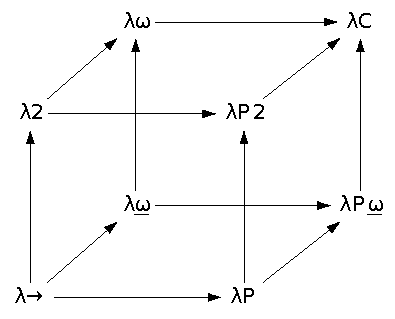
\includegraphics[width=6cm]{assets/Lambda_Cube.pdf}
  \caption{Lambda 方块}\label{fig:lambda-cube}
\end{wrapfigure}

关于不同类型论的表达力，我们可以在 Barendregt 提出的 Lambda Cube 中清晰比较。
从左下角到右上角，这一立方体代表的类型论的表达力逐渐增强，更具体的说，
x 轴的箭头 $\to$ 表示那些类型可以依赖值的类型论，属于依值类型\footnote{即依赖类型，此处为和下文区分做调整。}；
y 轴的箭头 $\uparrow$ 表示项可以依赖类型，即具备多态；
z 轴的箭头 $\nearrow$ 则表示类型可以依赖类型，即具备类型构造子。

在这一立方体中，$\lambda_\to$ 表示简单类型\lambdacalc（simply typed $\lambda$-calculus）、
$\lambda_2$ 表示 System F、$\lambda_\omega$ 表示 System $\mathsf{F}_\omega$\footnote{
  Haskell（GHC）使用这一系统，同时加上 ADT 和 Typal Equality.
}，而位居表达力顶端的类型论则是 Coquand 提出的 Calculus of (inductive) Constructions（$\lambda_\mathsf{C}$），被广泛的运用于
各个定理证明器中，包括 Coq 和 Lean.

而 \Tigris 使用的扩展 HM 系统则处于 $\lambda_\to$ 和 $\mathsf{F}_\omega$ 之间，这是因为我们虽然支持
直谓多态（predicative polymorphism，亦称 rank-1 polymorphism），我们并不支持 arbitrarily ranked 多态，
亦不支持非直谓多态（impredicative polymorphism），不满足 $\mathsf{F}$；此外其虽然支持 HKT，
但并不支持柯里化的类型构造子，因而最相似的类型论应当是 $\mathsf{F}_{\underline\omega}$. 但是即便如此，
我们认为 \Tigris 的类型系统的表达力已经胜过绝大多数具有多态的语言，因为无论是 Arbitrary-Ranked Polymorphism、
Impredicative types 还是 Higher-Kinded Types，都还停留在 PL 学术界阶段，并未得到
大规模的语言的支持。此外，\Tigrisd 的类型系统是 $\lambda_{\Pi\underline\omega}$ 与 $\lambda_{\Pi 2}$的简化混合体，
因为我们并未完全实现主流定理证明器所用的 CIC.

然而，类型论表达力的增强并非没有代价。Hindley-Milner 类型系统之所以经典，不仅仅是因为其开创性，
更因为它小心的设计。事实上，System $\mathsf{F}$ 及以上表达力的系统其
类型推论为不可判定（undecidable）且必须依赖用户的类型标注。对这些系统的推论/检查工作必须在本地通过
双向算法进行（local bidirectional type inference/checking）——即便是类型系统发达的
Haskell，也必须在使用上述高级特性时切换到另一个类型检查器——更不消说依赖类型论。
所以，即便 \Tigris 失去了很大程度的（逻辑上）的表达力，但考虑到本课题的编程子系统并不负责数学证明，
更不希望失去招牌的强大类型推论功能，我们认为这一表达力牺牲是完全值得的。

回到 IR 本身，之所以仍然选用 System $\mathsf{F}$ IR，是基于软件工程的认识：考虑本课题的未来展望，即便之后希望加上
上方的这些功能，我们也不需要耗费精力开展大型重构，可以在现有框架下直接进行补充。

同时，为了方便对编译器做 debug，我们利用与 Wadler 相似的 pretty-printing 算法打印 \texttt{FExpr} AST，
在前文的样例中亦有出现：输出结果与 \Tigris 的一个子集十分相似，同时还会添加必要的类型标注、类型 lambda 抽象与类型应用。
同样的打印算法也用于输出本文之后所描述的所有 IR 和 SBCL 目标代码。

类型系统、类型检查是 \Tigris \emph{极为重要}的组成部分。在下文我们会有更细节的论述。
\section{本章小结}（..略..）
\newpage
\thispagestyle{empty}
\null
\chapter{Type System of the \Tigris language}

\paragraph{命名方法} 在本节内，词语“约束”有广泛运用。因为我们实现的是基于约束求解的类型检查器，广义上的“约束”可以指
\begin{itemize}\itemsep0em
  \item 相等约束（equality constraint），具有自反性、交换性（虽然我们只用到其一侧方向）和传递性；
  \item 谓词约束（predicate constraint），具有累积性，主要体现在这种类型的约束是可以在类型模式中累积起来的。
\end{itemize}
虽然一些时候我们狭义地使用“约束”来特指含义二，
读者应当有能力根据上下文解读其具体含义。本文更多地使用广义上的“约束”一词。

简单的说，本类型系统实现称为约束变量求解实现，检查器称为约束变量求解器，在类型推断过程产生约束，
之后通过合一化进行求解。

\Tigris 实现了一个基于约束的 Hindley-Milner 类型系统，并添加了以下扩展功能：
\paragraph{谓词} 记作 \(C\ \bar{\alpha}\)，其中 $C$ 是谓词的头部。编译器在类型推论
阶段收集谓词信息，并在约束求解之后进行实例解析，并生成基于字典传递的实现代码。
\paragraph{严格高阶类型} 指的是高阶的 TV 和类型构造子必须完全应用。类型表达式 AST 中的
\texttt{KApp} 节点恰好足够实现这一功能，并使得诸如 \texttt{Functor}、\texttt{Monad} 之类的抽象（类型类）
能够在 \Tigris 中被定义，见 \autoref{fn:HKT}.
\paragraph{受限的 Rank-N Polymorphism} 指的是模式（\texttt{Scheme}）能够直接
嵌入类型表达式（通过 \texttt{TSch} AST 结点），但系统本身仍然是 Rank-1 Polymorphic 的。
这是因为我们通过 skolemization 的手段，对类型标注的检查做了精细控制。\footnote{
  且系统的自动泛化机制永远不会产生 higher-rank 类型。
}
这表示当检查 \(e : \sigma\) 时，我们用 skolem 常量\footnote{
  这些常量由 \texttt{TCon} 编码，即一个 0-元类型构造子。
}将 \(\sigma\) 实例化，
并检查其是否能和系统自身推断的类型合一化。不严谨但直观地说，
\begin{itemize}
  \item skolem TV 是刚性变量，主要表现在其独一无二，且无法同其他类型合一化；
  \item skolem TV 在实现中是通过维护一\emph{刚性变量集}确定的。这一集合用于拒绝错误的\emph{替换法则}（substitution），
    否则可能导致上述 skolems 逸出作用域，产生重大错误。
\end{itemize}
\paragraph{约束生成与求解} 约束的生成是通过类型推论进行的，且之后会在一次遍历后全部求解。求解器会返回
一个替换法则（即\emph{解}）与残余谓词约束，这些谓词约束最终会在被泛化的类型模式中出现。
\paragraph{Let-Polymorphism} 指的是由 Let-绑定的变量会依 TV s.t. $tv\notin\mathsf{ftv}\ \Gamma$ 被泛化，
同时其谓词约束（如果有）则会转变为对应类型模式的上下文。
非正式地说，表述
\begin{center}
  \underline{总是可以推断一个程序的类型，即便用户不提供任何签名}
\end{center}
是正确的，这一论断由 HM 系统的主类型特性所保证。

\section{形式文法}

类型系统是建构在核心代数上的：\Tigris 的核心代数是修改版的\lambdacalc。在描述这一类型系统的
行为规范（typing discipline）之前，我们首先给出核心代数、类型项的形式文法（formal grammar）。
\footnote{本文大多数文法，规则，都有其对应的 OTT 定义，Latex 源亦通过 OTT 生成。}
\nonterms{expr}
\nonterms{pattern}
%\nonterms{patmatrix}
%\nonterms{patbranch}
%\nonterms{tyctor}
%\nonterms{tyvar}
%\nonterms{tvset}
%\nonterms{tyargs}
\nonterms{typeexpr}
%\nonterms{predicate}
\nonterms{predicates}
\nonterms{scheme}
\nonterms{context}
\nonterms{constraint}
\nonterms{constraints}
\nonterms{subst}
%\nonterms{evidence}
%\nonterms{evctx}

\section{判断规则与推断规则}

现在，我们给出这一系统的判断规则（judgemental rules）与推断规则（inference rules）。每一条判断规则
都附带一段关于实现的解说。

\paragraph{合一化} 用于计算相等约束的一个最泛因子（most general unifier，MGU）。合一化引擎在类型检查阶段会
\begin{itemize}\itemsep0em
  \item 检查 TV 出现次数（occurrence）来防止无穷递归类型的产生，见小节 \ref{para:equirecursive}；
  \item 要求类型构造子应当完全匹配；
  \item 在两者元数相同的情况下将 \texttt{KApp} 与实际类型应用 \texttt{TApp} 合一化；
  \item 在结构性合一化类型模式前以$\alpha$-重命名之。
\end{itemize}
\drules[U]{\(\theta  \rpsym{=} \, \mathsf{unify} \, \rpsym{(}  \rpnt{ty_{{\mathrm{1}}}}  \rpsym{,}  \rpnt{ty_{{\mathrm{2}}}}  \rpsym{)}\)}{Unification of types}{Refl, VarL, VarR, Arrow, Prod}
\paragraph{约束求解} 是按从左到右的顺序进行的，这一过程会不断的累积替换法则；谓词约束也在这一阶段被收集并作为残余约束用于实例解析。
\drules[Slv]{\(\rpsym{(}  \theta  \rpsym{,}  \bar{\pi}  \rpsym{)}  \rpsym{=} \, \mathsf{solve} \, \rpsym{(}  \rpnt{C}  \rpsym{)}\)}{Constraint solving}{Empty, Eq, Pred}
\paragraph{实例化} 将绑定的 TV 替换为崭新（fresh）的 TV，同时返回必须满足的谓词约束。
\drules[Inst]{\(\rpsym{(}  \rpnt{ty}  \rpsym{,}  \bar{\pi}  \rpsym{)}  \rpsym{=} \, \mathsf{inst} \, \rpsym{(}  \rpnt{sch}  \rpsym{)}\)}{Scheme instantiation}{Forall}
\paragraph{泛化} 将所有给定环境内的非自由类型变量（quantified TV，qTV）提出，出现这些变量的谓词则会成为类型模式的上下文即
\underline{谓词会被\emph{保留}，当且仅当该谓词包含出现在结果类型中的 qTV. }

\drules[Gen]{\(\rpnt{sch}  \rpsym{=} \, \mathsf{gen} \, \rpsym{(}  \Gamma  \rpsym{,}  \rpnt{ty}  \rpsym{,}  \bar{\pi}  \rpsym{)}\)}{Generalization}{Gen}
\paragraph{表达式类型推断} 可以生成用于约束求解的约束，并通过求解这些约束（应用这些替换法则），以确定表达式的具体类型。
类型判断 \(\Gamma  \vdash  \rpnt{e}  \Rightarrow  \rpnt{ty}  \rpsym{;}  \rpnt{C}\) 读作:
\begin{center}
  \underline{
    在（类型）环境 $\Gamma$ 下，表达式 \(\rpnt{e}\) 具备类型 \(\rpnt{ty}\)，同时生成约束 \(\rpnt{C}\).
  }
\end{center}
根据核心代数，类型推断适用于：
\textbf{变量}：在 $\Gamma$ 中寻找并结果实例化类型模式；
\textbf{常量} 原本即有具体类型；
\textbf{Lambda 抽象} 其参数可获得崭新的 TV；
\textbf{函数应用} 生成能够让函数的参数类型与参数的类型相等的约束；
\textbf{元组} 生成能够让两个元组相同部分的类型相等的约束；
\textbf{条件表达式} 要求 then/else 分支类型相同，且要求条件为 \texttt{Bool}；
\textbf{Let 表达式} 推断/求解/泛化右手侧\emph{之后}再推断程序体；
\textbf{Letrec 表达式} \emph{首先}将与绑定 TV 数量相同的新 TV 推入 $\Gamma$ 内，
再推断每一个右手侧，并产生与推断的类型相等的约束；
\textbf{不动点组合子应用（Fix）} 即 \(\mathbf{fix}\ \lambda\ f.\ e\) 具有 \(\rpnt{e}\) 的类型；\footnote{
  虽然前文并未提到，但不动点组合子是 \Tigris 早期加入但不再维护的一项功能。其初衷是用于教学，
  但最后考虑实际效用便放弃维护。不动点组合子的语法是 \mintinline{ocaml}|rec expr|.
}
\subparagraph*{类型标注（Ascription）} 检查推断类型\emph{至少}与标注的类型具有相同的泛化程度，但根据
类型的 rank 使用不同的方法：
\begin{itemize}\itemsep0em
  \item 对 rank-1 类型标注而言，我们直接合一化；
  \item 对 rank-n 且 $n\ge 2$ 即类型模式含嵌套全称量化时，我们在类型推断与检查的四大步骤中做特殊对待：
  \begin{enumerate}\itemsep0em
      \item \textbf{实例化}\quad 将模式 \(\sigma = \forall \bar{\alpha}.\, \bar{\pi} \Rightarrow \tau\) 用
        崭新的 TV \(\bar{\beta}\) 实例化，得到 \(\tau_{\mathsf{inst}}\)；
      \item \textbf{约束求解}\quad 根据合一关系 $\tau_e \sim \tau_{\mathsf{inst}}$ 求解目前所有的约束，并得到
        一条替换法则 $\theta'$；\footnote{
          可以把这一步操作看作是一个\emph{过早的}求解（premature solving）。我们立即将之求解只是因为
          需要在之后的刚性检查中使用它们。
        }
      \item \textbf{刚性检查}\quad 对替换法则 $\theta'$ 中的每一个绑定 $\alpha \mapsto \tau'$，
        如果 $\alpha \in \rigid$，则 $\tau'$ 必须同 $\alpha$ 相等（注意：根据刚性变量的特征，即指其\emph{一定不能}被特殊化）。
        若这一检测不通过，则拒绝该类型标注并抛出合一化错误；
      \item \textbf{Skolemization}\quad 在前文与后文多次强调，用于保证标注的类型在泛性上与推断类型一致。
    \end{enumerate}
\end{itemize}
\subparagraph*{模式匹配} 对于某模式矩阵中的
\begin{itemize}\itemsep0em
  \item 每一分支 \(i\)：模式行向量 \(p_{i,1}, \ldots, p_{i,m}\) 会同
    被匹配对象（discriminant）的类型作比较；而 $\Gamma$ 则会由模式产生的绑定充盈，
    此外，模式产生的 TV 则会在其自身分支内被标记为刚性。通过这些机制，我们能够保证 TV 不会逸出到其他分支。\footnote{
      这一步操作可以看作是一个预防措施：此处所谓“逸出”只会在模式匹配枚举族类型的值时发生，而目前 \Tigris 并不支持。
    }
    每一分支的右手侧则会在上述过程之后推断，且要求（约束）所有分支具备相同类型。
  \item 每一被匹配对象 \(e_j\)：是各自\emph{独立}推断的，产生类型 \(\tau_1, \ldots, \tau_m\)，
    且这些类型必须同模式类型相同。
\end{itemize}
模式完全性、冗余性检查实际上在 System F 繁饰阶段进行而并非此处，因为两者需要类型信息：非完全模式产生编译器警告但并非错误；
冗余分支则立即从矩阵中移除。
{\allowdisplaybreaks
\drules[I]{\(\Gamma  \vdash  \rpnt{e}  \Rightarrow  \rpnt{ty}  \rpsym{;}  \rpnt{C}\)}{Constraint-based inference}{Var, Lam, App, Prod, Fix, Let, LetRec, Cond}
}
\begin{mathpar}
  \inferrule*[right=I-Match]
  {\Gamma \vdash e_j \Rightarrow \tau_j\,;\, C_j \quad (\forall j \in 1..m) \\
    \alpha = \fresh \\
    \text{For}\ i \in 1..k:  \\
    |(\bar{p}_i)| = m \\
    \Gamma \vdash p_{i,j} \Leftarrow \tau_j \Rightarrow \Gamma_{i,j}\,;\, C_{p_{i,j}}
    \quad (\forall j \in 1..m) \\
    \Gamma_i = \Gamma_{i,m} \\
    \bar{\beta}_i = \ftv(\bar{p}_i) \\
    \mathsf{pushRigid}(\bar{\beta}_i) \\
    \Gamma_i \vdash r_i \Rightarrow \tau_{r_i}\,;\, C_{r_i} \\
    \mathsf{popRigid}() \\\\
    C_{\mathsf{unify}} = \{ \tau_{r_i} \sim \alpha \mid i \in 1..k \} \\
    C = \bigcup_{j=1}^{m} C_j \cup
    \bigcup_{i=1}^{k} \left( \bigcup_{j=1}^{m} C_{p_{i,j}} \cup C_{r_i} \right) \cup
    C_{\mathsf{unify}}
  }
  {\Gamma \vdash \mathbf{match}\; e_1, \ldots, e_m\; \mathbf{with}\;
    \overline{\mid p_{1,1}, \ldots, p_{1,m} \to r_1}
  \Rightarrow \alpha\,;\, C}

  \inferrule*[right=I-Ascribe-Mono]
  {\Gamma \vdash e \Rightarrow \tau_e\,;\, C_e}
  {\Gamma \vdash (e : \tau) \Rightarrow \tau\,;\, C_e, \tau_e \sim \tau}

  \inferrule*[right=I-Ascribe-Poly]
  {\Gamma \vdash e \Rightarrow \tau_e\,;\, C_e \\
    \sigma = \forall \bar{\alpha}.\, \bar{\pi} \Rightarrow \tau \\
    \bar{\beta} = \fresh^{|\bar{\alpha}|} \\
    \theta = [\bar{\alpha} \mapsto \bar{\beta}] \\
    \tau_{\mathsf{inst}} = \theta(\tau) \\
    %%
    C_0 = \text{current constraints} \\
    (\theta', \_) = \solvesf(C_0, \tau_e \sim \tau_{\mathsf{inst}}) \\
    %%
    \rigid = \text{current rigid set} \\
    \forall (\alpha \mapsto \tau') \in \theta'.\;
    \alpha \in \rigid \implies \tau' = \alpha \\
    %%
    \tau_{\mathsf{sk}} = \skolem(\sigma) \\
    \text{add constraints for}\ \bar{\pi}
  }
  {\Gamma \vdash (e : \sigma) \Rightarrow \tau_{\mathsf{inst}}\,;\,
  C_e, \tau_e \sim \tau_{\mathsf{inst}}}
\end{mathpar}
由于\underline{模式匹配语句与类型标注}在 OTT 中不易正确表达，我们手动将其表示为\footnote{
  读者需要注意：这三条规则是手动排版的，一些符号并未在上述形式化文法中定义为生成规则，或者 OTT 源中的\emph{公式}（formula）。
  在这种情况下，我们使用恰当的自然语言直接在行内对之作出描述、定义。笔者只能怪罪其自身，因为他运用 OTT 并不很熟练。
}
其中 \rref{I-Ascribe-Poly, I-Ascribe-Mono} 正对应前文类型标注推断中表述的（非）泛情况。
\paragraph{模式} 可以绑定变量，亦可以从被匹配对象中产生新约束。判断规则
\(\Gamma  \vdash  \rpnt{pat}  \Rightarrow  \Gamma'  \rpsym{;}  \rpnt{C}  \rpsym{;}  \rpnt{ty}\) 读作：
\begin{center}
  \underline{
    模式 \(\rpnt{pat} : \rpnt{ty}\) 将 \(\Gamma\) 充盈（extend）为 \(\Gamma'\), 产生约束 \(\rpnt{C}\).
  }
\end{center}

\drules[P]{\(\Gamma  \vdash  \rpnt{pat}  \Rightarrow  \Gamma'  \rpsym{;}  \rpnt{C}  \rpsym{;}  \rpnt{ty}\)}{Pattern inference}{Wild, Var, ConstInt, ConstStr, ConstTrue, ConstFalse, ConstUnit, Prod}
因为构造子应用在 OTT 中不易表述，且可能存在可读性问题，仿照前文的形式，我们手动表述：
\begin{mathpar}
  \inferrule*[right=P-Ctor]
  {ctor :  \sigma \in \Gamma \\
    (\tau_{ctor}, \bar{\pi}) = \inst(\sigma) \\
    \peel(\tau_{ctor}) = (\tau_1, \ldots, \tau_n, \tau_{\mathsf{res}}) \\
    n = |\bar{p}| \\\\
    \Gamma_0 = \Gamma \\
    \Gamma_{i-1} \vdash p_i \Leftarrow \tau_i \Rightarrow \Gamma_i\,;\, C_i
    \quad (\forall i \in 1..n) \\
    C_{\pi} = \bar{\pi}
  }
  {\Gamma \vdash ctor\; p_1 \cdots p_n \Leftarrow \tau \Rightarrow \Gamma_n\,;\,
  C_1, \ldots, C_n, C_{\pi}, \tau \sim \tau_{\mathsf{res}}}
\end{mathpar}
其中 \(\peel\) 用于解构由箭头类型构成的树状数据结构（类型 AST），将之划分为\emph{参数类型}与\emph{结果类型}：
\[
  \peel(\tau_1 \to \tau_2 \to \cdots \to \tau_n \to \tau_r) = (\tau_1, \tau_2, \ldots, \tau_n, \tau_r)
\]
构造子的类型模式 \(\sigma\) 是从 \(\Gamma\) 中查找的，同时将用崭新 TV 实例化之。实例化产生的谓词约束
亦会被添加到类型环境中，保证类型类要求的正确传播。

下面，我们列出上文没有充分解说的一些概念。

\begin{definition}[Skolemization]
  将 TV 替换为 skolems 的过程，skolems 不能和除自身以外的任何类型合一化。
  \[
    \skolem(\forall \bar{\alpha}.\, \bar{\pi} \Rightarrow \tau) =
    [\bar{\alpha} \mapsto \overline{\mathsf{sk}_\alpha}](\tau)
  \]

  其中每一 \(\mathsf{sk}_\alpha\) 都是崭新的 skolem 常量（通过0-元类型构造子实现，
  在实现中有形式 \texttt{?sk.\(\alpha\)}）。
  “刚性”一词很好地表达了 skolem 的关键性质：
  \underline{\(\mathsf{sk}_\alpha \sim \tau\) 正确，当且仅当 \(\tau = \mathsf{sk}_\alpha\).}
\end{definition}

\begin{definition}[刚性变量集合/栈 rigid set/stack]
  \Tigris 的类型系统维护一个栈，其元素为一个个刚性变量集合
  （注意：这些集合是 $\rigid$ 的组成部分）。
  我们通过栈作为数据结构的特性自然地实现对嵌套作用域中的刚性变量的记录。这套系统有如下两个重要方法：
  \begin{align*}
    \pushRigid(\bar{\alpha}) &: \quad \rigid := \rigid \cup \bar{\alpha};\quad
    \mathit{stack} := \bar{\alpha} ::  \mathit{stack} \\
    \popRigid() &: \quad \mathbf{let}\; (S ::  \mathit{rest}) = \mathit{stack}\; \mathbf{in}\;
    \rigid := \rigid \setminus S;\quad
    \mathit{stack} := \mathit{rest}
  \end{align*}
  其中赋值操作 $(:=)$ 是由 \texttt{ST} 单子附带的，通过 \texttt{MonadStateOf} 接口实现。
  \begin{property}[Invariant]
    任一时刻，刚性变量集合 $\rigid$ 都具有以下性质：
    \[
      \rigid\equiv \bigcup stack
    \]
    即 $\rigid$ 是栈上的集合的并。在约束求解时，任一替换规则
    \(\alpha \mapsto \tau\) 满足 \(\alpha \in \rigid\) 和 \(\tau \neq \alpha\) 都将被拒绝。
  \end{property}
\end{definition}

\begin{remark}[求解刚性变量]
  约束变量求解器（即合一化求解过程）在遇到刚性变量时按以下规则工作：
  \begin{mathpar}
    \inferrule*[right=Solve-Rigid]
    {\alpha \in \rigid \\
    \tau \neq \alpha}
    {\solvesf(\alpha \sim \tau) = \mathbf{error}}

    \inferrule*[right=Solve-Rigid-Ok]
    {\alpha \in \rigid}
    {\solvesf(\alpha \sim \alpha) = \varnothing}
  \end{mathpar}
\end{remark}

尽管由于原生不动点组合子的存在，本系统已经存在矛盾，但只要不再使用这一已经不再被维护的功能，
系统仍然是合理的；此外，对 HM 系统添加的扩展也日渐影响着我们的类型系统的合理性。
本系统并不承担严谨的数学证明功能，因而“破坏合理性”从编程角度考虑，有程度之分。例如一个存在
矛盾的系统，如果不存在爆炸原理（ex falso quodlibet, EFQ）\footnote{
  即从矛盾能推任意命题。这一原理是类型论实现假命题（和空类型，不严谨的说，两者同构）的最简编码，其消去子：
  \begin{mathpar}
    \inferrule*[right=False-Elim]
    {\Gamma\vdash p : \mathsf{False}\\ \Gamma, x : \mathsf{False}\vdash C(x) : \mathbf{Sort}\ u}
    {\mathsf{False.rec}(p; C) : C(p)}

    \text{（无计算法则）}
  \end{mathpar}
  空类型的消去子是空完备（vacuously total）的：不需要分情况讨论，因为\emph{此处不存在任何情况}，
  因而，它不具备计算意义，也不能构造任何值（数据）。
}，则不一定能造成工程上的问题（例如 Java 与 Scala 的类型系统都已证明存在矛盾，但并不
作为能攻击它们安全性不好的理由）。

下面，我们论述本系统是通过何种机制保证合理性的。

\begin{property}[合理性 Soundness]
  \Tigris 通过以下若干机制保证其类型系统的合理性：
  \subparagraph*{Skolems} 类型检查器在遇到模式匹配和类型标注时，
  一些 TV 会被标注刚性并由 $\rigid$（在实现中是 \texttt{rTV}）记录。
  检查器通过拒绝将这些类型实例化到不相容（incompatible）类型的替换规则以避免不合理的泛化。
  \subparagraph*{Rank-N skolemization} 当检查 \(\rpnt{e} : \forall \, \rpnt{tv} . \pi \Rightarrow \rpnt{ty}\) 时, 我们用崭新
  的 skolem 常量替换 \(\rpnt{tv}\) ，以此来确保程序确实能对所有类型都工作——这一想法利用了全称量化的性质：如果表达式对任意类型都成立，
  则将之用任意独立不可合一的 skolem 实例化时也应当成立，因为该 skolem 是随机挑选的（崭新的），所以这是表达式成立的\emph{充要条件}。换句话说，
  如果这一检查失败，则说明表达式泛性不够强（not as generalized），与标注的类型不符合。
  \subparagraph*{存在次数检查} 是用来禁止用户构造等式递归（equirecursive）类型，比如
  \(\alpha \sim \alpha\to \beta\) 和 \(\alpha \sim \alpha\times\beta\)，对应非法的表达式
  \mintinline{lean4}|fun x => x x| 或
  \mintinline{lean4}{fun | (x, y) => x | z => z}.
  \subparagraph*{洁净（Hygienic）泛化} 只有 $\Gamma$ 中绑定的 TV 才会被泛化。
  谓词则根据前文描述的条件进行保留，以避免空约束。
  \subparagraph*{语法限制} 细心的读者如果详细地阅读了第一部分的类型表达式的 BNF 文法就会发现，
  目前的文法并不允许诸如 \((\forall a. a\to a)\to\mathsf{Int}\times \mathsf{Bool}\) 这样的 rank-2 type，
  即便类型表达式的 AST 定义中允许内嵌模式。的确，唯一能够引入内嵌模式的方法就是通过数据类型定义的多态栏位，
  而这一方式并不有害（在 Haskell98 中得到验证）。我们认为，这一条机制/限制是最强的，能够有效保证类型系统的合理性。
\end{property}

\begin{remark}[反例：为什么我们需要刚性变量]
  到目前为止，“刚性”一词出现过许多次，我们亦提到过为什么需要这样的机制，但仅局限于抽象的理论表述。
  下面提供若干反例，用具体例子展示刚性变量的必要性。
\begin{itemize}\itemsep0em
    \item \textbf{不正确实例化（Specialization）} 考虑
      \begin{minted}[frame=single]{lean4}
let id = (fun x => x : ∀a, a -> a) 1
 -- Can't unify type Int with ?sk.a.
let id' : ∀a, a -> a = fun x => (x : Int)
let id'' x : ∀a, a -> a = x + 1
      \end{minted}

      例子一合法：类型标注要求 \mintinline{lean4}|fun x => x| 是多态函数。根据整个定义，
      该函数被单态化（monomorphized）成 \texttt{Int}，相当于用户手动指导编译器
      将之实例化；

      而例子二非法：如果在函数体\emph{内} \mintinline{lean4}|fun x => ...| 内将 $a$
      （此时其为刚性变量）实例化为 \texttt{Int}（通过类型标注 \texttt{(x : Int)}）则不合理。
      这是因为，\texttt{id'} 由用户声明为多态函数，但其右手侧的定义则是单态函数，泛性不匹配；
      例子三同理。

    \item \textbf{泛性恢复（Polymorphism recovery）}
      一般来说，类型类的方法（其本身就很有可能是多态函数）在程序中是直接调用的，因而，我们
      参照 Haskell98 的特殊对待实现，在所有的方法调用处重新将之泛化。
      但考虑边界情况，如果用户希望直接使用（但不推荐）某个字典（实例）内的方法实现
      （\texttt{l} 是整数列表；\texttt{l'} 是字符串列表；\texttt{const} 是常函数，
      列表作为自函子的实现方法，即此处的 \texttt{f}，是列表映射 \texttt{List.map}）：
      \begin{minted}[frame=single]{ocaml}
let prog (Functor f) =
  let x = f (_ + 1) l and y = f (const ()) l'
  in (x, y)
      \end{minted}
      这同样也是被 Tigris 所支持的，但允许这种写法需要归功于刚性变量机制：$a$ 与 $b$ 在
      每次方法调用时都为刚性。这允许我们\emph{独立地}，在不同位置实例化之，比如上述例子中
      $f$ 在 $x$ 处有实例化 \([a\mapsto \mathsf{Int}, b\mapsto\mathsf{Int}]\)；
      在 $y$ 有实例化 \([a\mapsto \mathsf{String}, b\mapsto\mathsf{Unit}]\)：两个
      用例互不干扰。
  \end{itemize}
\end{remark}

\section{实例解析}
实例解析不仅仅是将实例与对应类型类配对。准确的说，编译器需要一套标准流程（算法）来为某个类的类型
寻找其对应实例。\footnote{
  PL 正式表述：找到一个见证（witness，即实现）谓词约束 \(\Pred = C\;\bar{\tau}\)
  的证据项（evidence term，即字典）。
} 这一标准流程称为\emph{实例解析}。下文叙述的算法从实例环境中搜索匹配的实例，并在链上递归地解析谓词约束
（例如前文出现过依赖其他实例的实例，这就产生了链）。

\paragraph{实例元数据} 每个记录的实例都是一个4-元组结构：
\[
  I = \inmark{\iname, \cls,\bar{\alpha},\bar{\pi}_{\ctx}}
\]
其中
\begin{itemize}\itemsep0em
  \item \(\iname\) 是该实例的独特标识符（命名例：\texttt{i\_Eq\_0}）；
  \item \(\cls\) 是类型类的头部；
  \item \(\bar{\alpha}\) 是实例声明中的类型参数；
  \item \(\bar{\pi}_{\ctx}\) 是实例的上下文（即依赖的其他实例）。
\end{itemize}
{
  例如，实例声明 \mintinline{lean4}|instance : forall α [Eq α], Eq (List α) = ... | 产生元数据
  \setlength{\abovedisplayskip}{6pt}
  \[
    I = \inmark{\texttt{i\_Eq\_1}, \texttt{Eq}, [\texttt{List}\;\alpha], [\texttt{Eq}\;\alpha]}
  \]
}

\paragraph{实例头部合一化（Head Unification）} 指的是检查某一目标（goal）\(C\;\bar{\tau}\) 是否可以被一个实例头部
匹配 \(C\;\bar\alpha\)。这一工作在进一步的实例解析前开展。

\begin{algorithm}
  \caption{Head Unification}
  \begin{algorithmic}[1]
    \Function{UnifyHead}{$\bar{\tau}_\mathsf{goal}, \bar{\alpha}_\mathsf{inst}$}
    \If{$|\bar{\tau}_{\mathsf{goal}}| \neq |\bar{\alpha}_{\mathsf{inst}}|$}
    \State \Return $\mathbf{error}$
    \EndIf
    \State $\theta \gets \varnothing$
    \For{$i \gets 1$ \textbf{to} $|\bar{\tau}_{\mathsf{goal}}|$}
    \State $\theta' \gets \unify(\apply(\theta, \tau_i), \apply(\theta, \alpha_i))$
    \State $\theta \gets \theta' \circ \theta$
    \EndFor
    \State \Return $\theta$
    \EndFunction
  \end{algorithmic}
\end{algorithm}

随着类型类定义、对应实例定义的增多，需要在环境中配对实例所需的时间就越久。因而，上面的合一化检查是一种\emph{剪枝}：
只要头部不匹配，则两者一定不能配对，则以这两者配对为目标的实例解析提前终止，编译器则继续往下寻找其他可以配对的实例。
显然，在找到正确实例之前的所有实例解析都不会返回结果，因而我们认为在这里做剪枝操作能够产生较大的优化成效。

\paragraph{实例解析算法}
主实例解析算法维护一个\emph{访问集}（visited set，$\Visited$）来检测链上的自环，表现为
解析结果歧义或环导致的解析不停机现象。

\begin{algorithm}\caption{Instance Resolution, Part 1}
  \begin{algorithmic}[1]
    \Function{Resolve}{$\Gamma, \Pred, \Visited$}
    \State \textbf{输入:} 环境 $\Gamma$，谓词 $\Pred = C\;\bar{\tau}$, 访问集 $\Visited$
    \State \textbf{输出:} 实例标识符 $e$ 使得 $e : C\;\bar{\tau}$；或报错
    \State
    \If{$\Pred \in \Visited$} \label{line:cycle}
    \State \Return $\mathbf{error}$:  ``cyclic instance resolution''
    \EndIf
    \State $\Visited \gets \Visited \cup \{\Pred\}$
    \State
    \State $\mathit{insts} \gets \Gamma.\instInfo[C]$ \Comment{类 $C$ 的所有实例}
    \If{$\mathit{insts} = \varnothing$}
    \State \Return $\mathbf{error}$: ``no instance for $\Pred$''
    \EndIf
    \algstore{instres}
  \end{algorithmic}
\end{algorithm}
{\footnotesize（接上图）}
\begin{algorithm}[H]\caption{Instance Resolution, Part 2}
  \begin{algorithmic}
    \algrestore{instres}
    \State
    \State $\mathit{found} \gets \mathbf{none}$
    \For{\textbf{each} $I = \inmark{\iname, C, \bar{\alpha}, \bar{\pi}_{\ctx}}$ \textbf{in} $\mathit{insts}$} \label{line:search}
    \State \textbf{try}:
    \State \quad $\theta \gets \Call{UnifyHead}{\bar{\tau}, \bar{\alpha}}$ \label{line:unify}
    \State \quad $\bar{\pi}'_{\ctx} \gets \apply(\theta, \bar{\pi}_{\ctx})$ \label{line:apply-ctx}
    \State \quad \textbf{for each} $\pi' \in \bar{\pi}'_{\ctx}$ \textbf{do} \label{line:recurse}
    \State \quad\quad $\_ \gets \Call{Resolve}{\Gamma, \pi', \Visited}$ \Comment{保证可解}
    \State \quad \textbf{end for}
    \State \quad $e \gets (\iname :  C\;\bar{\tau})$ \Comment{引用实例的类型标注} \label{line:evidence}
    \State \quad \textbf{if} $\mathit{found} \neq \mathbf{none}$ \textbf{then} \label{line:ambig}
    \State \quad\quad \Return $\mathbf{error}$:  ``ambiguous instance for $\Pred$''
    \State \quad \textbf{end if}
    \State \quad $\mathit{found} \gets \mathbf{some}(e)$
    \State \textbf{catch}:  \textbf{continue} \Comment{捕捉错误，即解析失败，尝试下个实例}
    \EndFor
    \State
    \If{$\mathit{found} = \mathbf{none}$}
    \State \Return $\mathbf{error}$:  ``no matching instance for $\Pred$''
    \EndIf
    \State \Return $\mathit{found}$
    \EndFunction
  \end{algorithmic}
\end{algorithm}

\begin{remark}[$\mathsf{ResolveM}$]
  上述算法运行在 \texttt{ResolveM} 单子中。正如之前我们提到过的类型检查器的 \texttt{InferC}
  单子一样，这里的 \texttt{ResolveM} 定义不过是把状态变成了 \texttt{ResolveState}，
  即上述 $\Visited$，但在实现上我们使用哈希表实现的集合 \texttt{HashSet} 作为容器储存谓词。
  \begin{Verbatim}[numbers=left,baselinestretch=1]
    abbrev ResolveState := Std.HashSet Pred
    instance : MonadLift (Except TypingError) (EST TypingError σ) where
      monadLift
      | .error e => throw e
      | .ok e => return e
  \end{Verbatim}
  同时，我们为这一单子实现 \texttt{MonadLift} 接口，以定义从错误处理单子 \texttt{Except} 到 \texttt{EST} 的\emph{自然变换}\footnote{
    自然变换是范畴论的概念。函数式编程的定义与其在数学中类似：将一个在单子 $m$ 中运行的操作提升进 $n$ 中，有方法
    $\mathsf{liftM} : m\ \alpha\to n\ \alpha$. 在 Lean 中，这一变换不需用户显式写出，是自动插入的；但实例本身需要用户自行定义。
  }
  （natural transformation），
  将任何可能报错的纯函数（操作）提升（lift）到后者中以运行。
\end{remark}

\begin{property}
  下面，我们给出实例解析算法的一些性质。
  {\setlength{\parskip}{-1em}
    \subparagraph{停机性（Termination）} 还没有被证明，从源代码定义中的 \texttt{partial} 关键字亦可看出。
    直观的讲，实例解析停机当且仅当某一实例链是良基的，即不存在环。集合 $\Visited$（第 \ref{line:cycle} 行）虽然可以
    检测直接的环（自环），但并不一定能够保证停机，尤其是针对一些边界情况。
    \subparagraph{语义一致性（Semantic Consistencies）} 是通过\emph{单一匹配}原则保证的：如果有多个实例匹配一个目标（第 \ref{line:ambig} 行），
    解析算法将抛出歧义错误。这告诉我们一个重要性质：程序的意义不会受到\underline{随机选择的实例影响，因为解析过程不随机选择实例}。
    然而与常规实现不同，这一原则适用所有实例，与实例本身的泛性无关：也就是说，若存在多个匹配的实例，且存在其中之一最“具体”的实例
    也不会导致其被优先选择，而是出现歧义错误，尽管优先选择它在工程意义上看起来更合理。若允许多个匹配实例的存在，
    其中一个做法是加入优先级和默认实例，但目前我们还不支持。
    \subparagraph{证据生成（Evidence Generation）} 指以下类型标注的实例标识符 $e = (\iname : C\;\bar{\tau})$
    其之后在 System F IR 翻译阶段将被繁饰到字典传递风格的实现，并用字典投影结点 \texttt{Proj} 编码。
    \subparagraph{上下文传播（Context Propagation）} 指对具有上下文谓词（依赖其他实例的实例）的实例 $\bar{\pi}_{\ctx}$
    使用合一化产生的替换法则实例化所有的上下文谓词（第 \ref{line:apply-ctx} 行），并
    递归地解析它们（第 \ref{line:recurse} 行）。例如
    \mintinline{lean4}|instance ∀α [Eq α], Eq (List α) = ..| 中的 \texttt{Eq a} 即为
    一上下文谓词（显然，很多时候上下文谓词不止一个）。
  }
\end{property}

为了加深对算法的理解，我们用一个简单的例子模拟实例解析算法。考虑解析 $\mathsf{Eq}\;(\mathsf{List}\;\mathsf{Int})$，给定实例环境如下:
\begin{align*}
  I_0 = \inmark{\texttt{i\_Eq\_0}, \mathsf{Eq}, [\mathsf{Int}], \varnothing}, &&
  I_1 = \inmark{\texttt{i\_Eq\_1}, \mathsf{Eq}, [\mathsf{List}\;\alpha], [\mathsf{Eq}\;\alpha]}.
\end{align*}

\begin{enumerate}\itemsep0em
  \item 目标: $\mathsf{Eq}\;(\mathsf{List}\;\mathsf{Int})$
  \item 尝试 $I_0$：$\unify(\mathsf{List}\;\mathsf{Int}, \mathsf{Int})$，失败
  \item 尝试 $I_1$：$\unify(\mathsf{List}\;\mathsf{Int}, \mathsf{List}\;\alpha)$，由 $\theta = [\alpha \mapsto \mathsf{Int}]$ 成功
  \item 上下文: $\apply(\theta, [\mathsf{Eq}\;\alpha]) = [\mathsf{Eq}\;\mathsf{Int}]$
  \item 递归地解析 $\mathsf{Eq}\;\mathsf{Int}$:
  \begin{enumerate}\itemsep0em
      \item 尝试 $I_0$: $\unify(\mathsf{Int}, \mathsf{Int})$，由 $\theta = \varnothing$ 成功
      \item Return $(\texttt{i\_Eq\_0} : \mathsf{Eq}\;\mathsf{Int})$
      \item 上下文: $\varnothing$，为空则不再需要递归
    \end{enumerate}
  \item 返回 $(\texttt{i\_Eq\_1} :  \mathsf{Eq}\;(\mathsf{List}\;\mathsf{Int}))$
\end{enumerate}

\begin{remark}[与 GHC 的比较]
  类型类由 P. Wadler 提出，并最先应用于 Haskell 语言。作为其最流行的实现，
  GHC 实现了一个健壮性（robust）更强，更加复杂，且具备语言标准中未提及的许多扩展的类型类机制。虽然 \Tigris 类型类的实现从
  GHC 学习、汲取了诸多灵感，但必须承认相比于后者，前者的实例解析策略要简单得多：
\begin{itemize}\itemsep0em
    \item \Tigris 不允许重叠实例，无论这些实例在源代码中出现的先后顺序；GHC 则提供一套实例优先级机制，
      允许用户针对实例解析做高细粒度的控制。
    \item 此外，\Tigris 不允许针对实例设置后备（fallback）实例。
  \end{itemize}
  但是，若和 Haskell98 或 2010 做比较，
  \Tigris 的实例声明在一些地方反而更具表达性：譬如我们部分实现了 GHC 语言扩展 \texttt{FlexibleContext}\footnote{
    这一扩展解除了 Haskell98 的限制，不再要求谓词约束必须具有 \texttt{class type-variable} 或
    \texttt{class (type-variable type1 type2 .. typen)} 的形式。
  }，因而可以定义一些形式不同的实例，例如\mintinline{lean4}|instance ∀a [Eq a], Eq (a * a) = ..|. 此外，多类型参数
  的类型类亦支持，比如前文曾出现过的 \texttt{HAdd} 和 \texttt{HEq} 的例子。
\end{remark}

\section{System F 繁饰}
带类型的语法树（typed syntax）\texttt{TExpr}，在经历实例解析的同时，也正在被繁饰到 \texttt{FExpr}.
下面就这一过程进行直观的探讨。在这一部分我们侧重谈实现，更多的使用“字典”一词表示某接口（类）的实现。
首先给出繁饰的具体行为：

给定一模式
\[
  \forall \alpha_1 \cdots \alpha_n [P_1, \dots, P_k], \tau
\]
我们将一个绑定的右手侧翻译为
\begin{equation}
  \Lambda \alpha_1,\dots,\alpha_n.\lambda d_1,\dots,d_k.\ body
\end{equation}
其中 $d_1,\dots,d_k$ 是谓词 $P_1,\dots,P_k$ 对应的实例。若右手侧已经由正好 $k$ 个字典 lambda
（即绑定字典的 lambda 抽象）起头，且这些字典 lambda 是编译器自动为类型类方法生成的封装，则这种情况下
只在头部添加 \texttt{TyLams}.
每当繁饰过程遇到一个 \texttt{Var} 结点 $\mathsf{Var}\ x:\sigma$ 其中 $\sigma = \forall \bar{\alpha}\ \bar{P},\, tbody$
时，会繁饰为
\begin{equation}
  \begin{split}
    &\Tyapp\ \cdots\ (\Tyapp\ (\FVar\ x\ ty_\mathsf{mono})\ \alpha_1)\ \cdots\ \alpha_n\\
    &\mathsf{App}\ \cdots\ d_1\\
    &\vdots\\
    &\mathsf{App}\ \cdots\ d_k
  \end{split}
\end{equation}

字典参数\footnote{标识符为 $\mathtt{d}\texttt{\_}P\mathtt{.cls}\texttt{\_}{i}$，其中 $P$ 是谓词, $i$ 是
该类型类的实例计数器；若这一字典参数是持久化的，则在其之前加字符 \texttt{r}.}是以下两种情况之一
\begin{itemize}\itemsep0em
  \item 存在于作用域内，也就是说，与某一由上述字典 lambda 产生的谓词模板相匹配；或，
  \item 由实例解析过程合成（synthesized），产生一个不带类型的表达式（\texttt{Expr}）。
    我们在该表达式上重新做类型推断与字典繁饰，以转变为 \texttt{FExpr}. 这一过程显然是递归的。
\end{itemize}

若某一方法具有多态类型，例如 \texttt{Functor} 的 \texttt{map}，或者从实现上说，\texttt{TSch (Forall as [] τ)}，
则其将被\emph{实化}（reified）到 System F 的类型抽象（type abstraction，即 type lambda），这一转变是通过将其所有的
$\forall$ binder 一一包裹在 \texttt{TyLam} 结点中而达成的。对于以后计划实现 Higer-Ranked 类型时同理。但需要注意，
各方法独自的谓词上下文（例如，\texttt{map} 方法依赖某一接口）目前还不支持，且若出现则会抛出错误。

\paragraph{字典持久化} 指的是将合成的字典持久化的优化。实践证明，绝大多数情况下同一字典
都在代码中使用多次，如果每次使用都需要重新合成相同的字典，或生成\underline{字典间的应用}（如果实例具备上下文），
则编译效率就比较低下。持久化通过在函数层级记录每个字典的第一次使用，在遇到同一字典多次使用时，重复使用第一次合成的字典，来提高性能。
而语言自带的 Let-绑定正为这一优化铺平了道路：我们在函数头部插入一个 Let-绑定，将所有行内使用到的字典提出（hoist）并用 Let 绑定之。
从语义上讲，字典持久化类似\emph{公共子表达式消除}（common subexpression elimination），只不过字典是很特定的语言对象，因而使得
优化实现起来简单。我们用一个稍复杂的例子（简单例子不需优化） \texttt{Functor}、 \texttt{Applicative}、\texttt{Monad}
作为代数结构的继承关系来展示这个优化：
\begin{minted}[frame=single]{lean4}
class Applicative (f : 1) =
  { pure : ∀ a, a -> f a
  , seq : ∀a b, f (a -> b) -> f a -> f b}
class Monad (m : 1) =
  { bind : ∀a b, m a -> (a -> m b) -> m b
  , return : ∀a, a -> m a}
infixl 55 ">>=" => bind ;; infixr 60 "<*>" => seq
instance ∀(m : 1) [Monad m], Applicative m =
  { pure = return
  , seq f x = f >>= fun f => x >>= fun x => return $ f x}
instance ∀(f : 1) [Applicative f], Functor f = {map f x = pure f <*> x}
instance Monad Option =
  {return = Some, bind | None, _ => None | Some x, f => f x}
let seqOp = (Some id <*> _)
\end{minted}
已知 \texttt{i\_Monad\_0, i\_Applicative\_0} 分别是 \texttt{Option} 作为 \texttt{Monad}、
\texttt{Monad} 作为 \texttt{Applicative} 的实例，则有 IR 结果

\begin{minted}[ignorelexererrors=true]{ocaml}
let seqOp : ∀ α, (Unit → Option α) → Option α =
  let rd_Applicative_1 : Applicative Option =
    let rd_Monad_0 : Monad Option = i_Monad_0
    in i_Applicative_0@Option rd_Monad_0
  in (Λ α. rd_Applicative_1[1, seq]@Option (Some@(α → α) id@α))
\end{minted}

如上所示，持久化优化被触发，两个字典及其应用，都通过 Let 缓存（cached）于函数头部，且
绑定的标识符为 \texttt{rd\_Applicative\_1}. 注意到其计数器为 $1$，这说明持久化优化在机制上
会合成新的字典（但效率远高于正常合成步骤）。所以我们认为，在繁饰过程中加入这个优化，实现简单
且十分实用，能够切实提高编译性能。

繁饰过程运行在 $\mathsf{F}$ 单子中。这一单子与前面提到的单子相似，但包含繁饰需要的特定状态类型。
但不同于以往，$\mathsf{F}$ 基于 \texttt{EStateM}，一个自带错误处理与（用纯函数模拟的）的可变状态的单子，
而非之前真正具备（线程独立的）可变状态的 \texttt{ST}. 这样设计，是因为繁饰过程涉及到许多\emph{本地状态}，
搭配递归调用，我们不必次次修改可变状态，而是在调用处传入这一调用所需的本地状态即可，这
在底层是通过栈分配的函数参数实现的。

如同之前的抽象语法树，System F IR 也使用类 Wadler 的 pretty printing 算法，方便 debug 和
教学使用。

我们以笔者对这一模块设计上的考量与反思总结本部分。
\begin{remark}[System F IR 的实用性与设计上的反思]
  自本课题开题伊始，笔者本人对 \Tigris 的目标便十分明确：编译到 Common Lisp. LISP 是
  动态类型语言，而最流行的 SBCL 实现则自带一些类型推断（但大概率不是 gradual typing）、传播的扩展功能，
  因而我们做\emph{泛型特殊化}、或将类型传播到下一个降级阶段（即下文的 Lambda IR 降级）的理由不是很充分。\footnote{
    虽然之后的编程实践证明，带着类型走完全部编译流程是极方便的，且更加可靠。
  }

  因为这些考量，我们其实并不需要上文的 System F IR，因为没有它类型类繁饰也能实现，但最终仍然保留了这一 IR.
  笔者需要承认，这里既有一些设计上的前瞻性，也有设计失误、考虑不够充分的问题：
\begin{itemize}\itemsep0em
    \item 前者表现在若我们之后需要实现 arbitrary rank polymorphism 和 inductive families 时很自然：可以由当前的 IR 编码。
    \item 后者表现在下文的 Lambda IR 中。在设计 Lambda IR 时我们没有考虑将 System F IR 的类型信息携带到下一层级，因而
      Lambda IR 不带类型信息，直接导致后端代码生成时的附加困难，更使得后端实现的健壮性成疑。目前的后端会通过收集
      变量的\emph{形状}来产生代码，但这并不可靠，且存在一些笔者临时修补的错误。不仅如此，若后期我们需要添加静态类型语言后端，
      比如 C，这一 IR 就几乎不可用。
  \end{itemize}
  虽然此处的问题和 System F IR 联系不深，但优点抑或缺陷，都向我们揭示了
  一个宝贵的教训：
  \begin{center}
    \underline{在任意编译阶段，都应当具备携带类型的 IR.}
  \end{center}
\end{remark}

\section{本章小结}（略）

%\newpage
%\thispagestyle{empty}
%\null
\chapter{The \Lambdair, CPS, Codegen \& FFI}
System F IR 的繁饰标志着编译“上升期”的结束；\Lambdair\footnote{
  \Lambdair 是致敬 Appel 在其工作 \emph{Compiling with Continuations}（可能也包括 SML/NJ 编译器）使用的同名 IR；
  \Tigris 本身则是致敬 Appel 的 \emph{Modern Compiler Implementation in ML}，昵称\emph{虎书}，因为其封面有一只老虎。
  \Tigris 有拉丁语的老虎之意。
}则作为一个真正的中间表示（intermediate representation, IR），标志着编译“下降期”（降级）的开始。
\Lambdair 应当算做 ANF，后者是函数式语言编译器常用的一类 IR.

ANF 的精髓在于\emph{变量}。在 ANF 中，某一语言对象，或（非基础的，nontrivial）表达式，都由 Let-绑定捕捉为变量，
并通过后者指代：这一特性在某种程度上与汇编代码类似。虽然 \Tigris 编译到高级语言，但其后端代码风格
与手写程序不同，因而 SBCL 可以从中获得一定优势，相当于 \Tigris 编译器已经帮其做了部分工作。

\section{\Lambdair}
\paragraph{\Lambdair 的定义}
\Lambdair 的设计从六大角度开展：值、右手侧、陈述语句、尾调用位置、表达式、函数。对应到实际实现，就是
\texttt{Value}、\texttt{Rhs}、\texttt{Stmt}、\texttt{Tail}、\texttt{LExpr}、\texttt{LFun}，我们将逐一介绍
各个部分。\underline{读者应当注意上述六个类型是互递归的。}
{\setlength{\parskip}{-1em}
  \subparagraph*{\texttt{Value}} 也叫立即数/值，不能再化简。
  立即数包括变量、常量（整数、字符串、布尔值、幺元）、构造值和 Lambda 抽象。应当注意，
  此时的 Lambda 抽象还并没有经过闭包转换，因此可以捕捉自由变量。
  \subparagraph*{\texttt{Rhs}} 指 ANF 的右手侧，且只能以变量作为参数。
  右手侧包含原生函数（整数四则运算、常量的等号）、字典投影、元组、构造子应用（在定义上与立即值的构造值一致，但意义不同）、
  构造子测试（即测试两构造子是否相同）与函数调用。
  \subparagraph*{\texttt{Stmt}} 指陈述语句，目前只有 Let1.
  \subparagraph*{\texttt{Tail}} 表示尾调用位置，即某一函数的最后一条语句（一个操作）
  但不仅包括函数调用，还有函数返回、条件表达式、多分支条件匹配表达式（switch）和一特殊 token \texttt{MATCHFAIL}. \texttt{Tail} 具有标注
  尾调用位置的重要功能，方便后期做尾调用优化。在具体实现中，switch 语句又依匹配对象不同分为常量、构造值两类——这样的区分
  有利于后期更方便地做常量折叠优化。
  此外，\texttt{MATCHFAIL} 是一特殊常量，用于表示不完全模式匹配的后备分支。如前文所述，若进入这个分支，则程序立即抛出错误并终止。
  在具体实现中，其能够接收一个被匹配对象变量名的参数，后者会传递到并用于后端代码生成，以产生更好定位的错误信息。
}
\subparagraph{\texttt{LExpr} 与 \texttt{LFun}} 前者是 \Lambdair 程序的主体，包含序列操作、
立即数 Let-绑定（记 $\mathbf{let}_\iota$）、右手侧 Let-绑定（记 $\mathbf{let}$）、LetRec-绑定（记 $\mathbf{let}_\omega$）：三种 Let 因其右手侧不同而不同，
分别是 \texttt{Value}、\texttt{Rhs} 和递归定义。

\texttt{LFun} 则表示 IR 中的一个顶层函数，
是一个3-元组 \texttt{(fid, param, body)}，
分别代表函数名、参数名和函数体（\texttt{LExpr}）。
在具体实现中，LetRec-绑定携带一列顶层函数（\texttt{LFun}），而非 \mintinline{lean4}|Name × Name × LExpr|，即便
LetRec 绑定的是本地函数。原因完全是性能上的，因为两者具有相容的表示，直接使用前者替代后者能够省去两种类型之间多余的转换。

尽管 \Tigris 是纯函数式语言，我们仍用序列操作 \texttt{seq} 来捕捉尾调用 \texttt{Tail}。这是因为具体实现中，只有 \texttt{seq} 结点
能够携带尾调用信息。而且，考虑到以后可能为 \Tigris 加入不纯模式，将其转变为类似 OCaml 的语言，具备 \texttt{seq} 结点
可以减轻工作量。

\Lambdair 沿用前述的 pretty-printing 算法，但因为篇幅限制，我们不再给出范例。读者只需知道其语法类似 Haskell 和 SML 的混合体即可。

IR 降级的过程中有一些很可注意的细节。下面针对降级期间的特殊情形作探讨。

\paragraph{捷径: 构造子与原生操作}
\Tigris 的七种原生操作与0-元构造子不存在函数调用产生的性能损失，而原生调用的检测则是通过语法树上的模式匹配实现的。
因而有时需要做 $\eta$-expand，否则可能出现漏检情况。具体实现中，无论是原生操作还是普通函数，对降级过程而言都是相同的，径由
\texttt{App} 分支，但很明显特殊对待前者能够获得更好的性能——目前两者唯一的区别就是其标识符——通过在降级最开始的位置匹配这些标识符，
我们即可优先处理原生调用，避免普通调用产生的性能损失（目前编译器未做内联优化）。

\begin{minted}[numbers=left,baselinestretch=1]{lean4}
partial def lowerF (e : FExpr) (ρ : Env) (ctors : Std.HashMap String Nat)
  (k : Name -> M σ LExpr) : M σ LExpr := do
  match matchBinaryPrim e with
  | some (op, x, y) =>
    lowerF x ρ ctors fun vx =>
      lowerF y ρ ctors fun vy => do
        let r <- fresh "p"
        let cont <- k r
        return .letRhs r (.prim op #[vx, vy]) cont
  | none => (...) -- 此处处理构造子（与上同）和普通降级
\end{minted}

\paragraph{字典投影} 如前文所述，是专门为类型类方法设计的。根据最原始的字典传递实现，
方法是通过模式匹配投影出来的。这不仅增加代码生成体积，亦容易复杂化降级过程。因而我们在前文引入这一结点，并在
\Lambdair 的降级过程中传递，最后在后端直接生成投影代码，避免经过模式匹配。

\paragraph{函数，函数应用与逆柯里化}\label{sbcl:cav} 函数式语言通常保证柯里化。但当我们考虑
生成代码时，就不得不注意其带来的性能问题——为 $n$-元函数产生 $n$ 个函数显然是不现实且臃肿、低效的，同时还增加目标语言做
尾递归优化的难度。因而绝大多数以函数作为头等对象的语言（广义上的函数式语言）都做逆柯里化（uncurrying）优化。该优化通过将连续的
函数头（柯里化满足这一特征）压缩成一个 $n$-元组作为单参数（这是我们的具体实现）以便被编码为立即值 \texttt{Value} 并简化柯里化函数的 IR 降级。
有以下若干值得注意的概念：

{\bf 解构连续函数头} 是用于压缩（squash）具有连续函数头（无论是否由柯里化造成）的函数，例如 \mintinline{lean4}|fun x => fun y => ...|，
并返回 3-元组 \texttt{(p0, rest, core)}，分别指代函数首参数、剩余参数与函数体。

{\bf $\eta$-expansion} 不仅仅指 \lambdacalc 中的计算法则，在此处更指用于解决降级的函数应用（\texttt{App}）分支并未正确
处理的边界情况。考虑应用通过模式匹配投影产生的函数，如
\begin{minted}[frame=single]{ocaml}
let boxed = Boxed (_ + _) and unwrap (Boxed f) = f
in unwrap boxed 20 20
\end{minted}
其中 \texttt{unwrap boxed 20 20} 称为\emph{高阶应用}（higher-order application）：\texttt{boxed} 的应用在 Let 程序体内发生，但
并不能被降级过程捕捉，因为只有应用头 \texttt{unwrap} 对其可见，且 \texttt{unwrap} 是一高阶函数（即它返回函数，但其函数体内没有应用），
因而这条语句其实发生\emph{两次}函数应用，但降级过程只可见第一次；图 \ref{fig:higher-order} 形象地给出了两次函数应用。
\begin{figure}[H]
  \[
    \begin{tikzcd}
      {\mathsf{unwrap}} && {\mathsf{boxed}} && {20\ 20}
      \arrow[""{name=0, anchor=center, inner sep=0}, "{\text{\textcircled{\tiny 1}}}"', curve={height=-18pt}, from=1-1, to=1-3]
      \arrow["{\text{\textcircled{\tiny 2}}}", curve={height=-30pt}, Rightarrow, from=0, to=1-5]
    \end{tikzcd}
  \]
  \caption{高阶应用}\label{fig:higher-order}
\end{figure}
应用\textcircled{\scriptsize 1}对降级过程可见，但是，\underline{由其\emph{返回的函数产生的}应用\textcircled{\scriptsize 2}对降级不可见}。
因而，\texttt{unwrap}在这一过程中会 $\eta$-expand 为 \mintinline{ocaml}|let unwrap (Boxed f) x y = f x y|，显式化
高阶应用。$\eta$-expansion 过程产生的参数有 $..\eta N$ 的形式，例如 \texttt{\_pR\#η0}.
熟悉\lambdacalc 的读者或许知道 $\eta$-expansion 可能在 CBV 下带来意想不到的求值语义——譬如上文提到的
$\mathsf{Y}$ 组合子的 Church 实现若不加更改，在 CBV 下\emph{不会停机}，但 $\eta$-expansion 推翻了这一结论，
产生\emph{语义不一致}问题——且我们无法避免其发生。因此，与其无条件地做 $\eta$-expansion，我们只对
上面这种情况特殊处理，其余不变，以期尽可能减少对于语义的影响。

此外 Lean 亦有 $\eta$-expansion 导致语义不一致的问题，但由于危害不大，其开发者目前也不准备对此做任何处理。
见脚注笔者发表的 Proofexchange 帖子\footnote{\url{https://proofassistants.stackexchange.com/a/4424}}，
以及帖子中 Lean 类型论设计者的回答和 GitHub issue \texttt{\#5908}\footnote{\url{https://github.com/leanprover/lean4/issues/5908}}.

{\bf 语法元数（syntactic arity）} 指的是用户在函数定义时给出的元数。问题在于将不同种类的元数同上述的高阶应用/函数混搭时
易出现问题，而函数式语言恰巧存在大量此种风格的程序。一般来说，降级工作通过检查函数对应的类型来决定函数的元数——实践中发现这一检查并不足够。
考虑上文的 $\mathsf{unwrap} : \mathsf{BoxedAdd}\to\Int\to\Int\to\Int$，从类型上看应为 3-元函数（由于柯里化），但根据用户给出的定义，其实际上只接受一个参数——
即便传给其另外两个参数，它也不知道该怎么办——因为其函数体根本没有出现另外的参数。因而，只有在经过 $\eta$-expansion 后它才能够是真正的 3-元函数。相比于类型决定的元数，
在逆柯里化工作中，我们更多依靠语法元数。

{\bf 逆柯里化投影生成} 指的是为逆柯里化的函数生成投影代码的过程。因为我们使用元组来实现逆柯里化，因而
在函数实际要使用传入的参数时需要首先将其投影出来。这一变换通常与闭包转换一起进行，在下文介绍。

{\bf 栈底层降级工作} CPS 风格的递归代码在降级过程中是经常使用的，而递归的首要工作就是明确基准情况（base case）——续点栈（continuation stack）底层的
降级工作 \texttt{lowerFCore} 所表示的就是这一情况。\texttt{lowerFCore} 可以看作和 IR 中的 \texttt{Tail} 存在\emph{同像性}（homoiconicity）\footnote{确切的说，和第二部分提到的 \texttt{chainl/chainr} 的一致，这也是一种\emph{同态}。}，因为
从降级工作的角度，或是 IR（即 object language，数理逻辑上的\emph{对象语言}）的角度而言，两者都代表尾调用——\underline{\texttt{lowerFCore} 本身也用于 \texttt{Tail} 的降级}。
\begin{minted}[escapeinside=`',numbers=left,baselinestretch=1]{lean4}
def lowerFCore (e : FExpr) (ρ : Env) (ctors : HashMap String Nat) : M σ LExpr :=
  lowerF e ρ ctors $ pure `$\circ$' .seq #[] `$\circ$' .ret
\end{minted}
其中 $(\circ)$ 表示函数复合运算符，在函数式语言中十分常见。对比之可以发现，
栈底层的降级 \texttt{lowerF} 不需要传入续点 $k :\mathsf{Name}\to\mathsf{M}\;\sigma\;\mathsf{LExpr}$，因而不存在由续点造成的\emph{控制转移}（control transfer）。
我们将在 CPS 化一节中谈到续点、续点传递（化）的概念。

实现逆柯里化是在函数定义和函数应用上共同努力的结果——不妨先定义逆柯里化函数的参数安排（layout）。对于某 $n$-元函数的参数 $a_1,\dots,a_n$，构造 $pl$（payload）其中

\begin{equation}
  pl =
  \begin{cases}
    ((), ()) & n = 1, a_1 = ()\\
    (a_1, ()) & n = 1\\
    (a_1,\dots,a_n) & n \ge 2
  \end{cases}
\end{equation}

笔者必须承认，事后考虑起来，这一 layout 存在一些设计问题。虽然它是元组，但编码上其与 \texttt{List} 相仿，比如单元素时
在元组尾端加入了一个哨兵幺元（sentinel），但在 $n\ge 2$ 时又将之去掉。如果——且恰巧——没有类型信息的辅助，
要判断这一元组的形状较难，为后端代码生成徒增麻烦。此外，我们还应当在编译器前端就将语法元数收集起来，
而不是在这一阶段按需收集，导致代码的可维护性下降。

从函数应用的角度考虑，逆柯里化的函数在应用时必须区分\emph{完全应用}与\emph{部分应用}。我们的做法是分情况讨论：
对于前者，分为单参数、类型/语法元数不匹配两种情况进行处理；
对于后者，根据缺少的部分计算需要补充的元数，并根据数目封装一层新 Lambda 抽象。
同理，对于函数形式的值——构造子，我们也采取相同的操作。但由于构造子毕竟不是函数，
不具备函数体，仅仅是能够应用，则处理起来相对简单许多。

\paragraph{模式匹配} 是通过决策树算法\footnote{
  从实现上看，完全/冗余性检查可以看作是这一算法的超轻量版本。
}
开展编译工作的。我们定义三种类型 \texttt{Sel}、\texttt{RowState}、\texttt{DTree}，分别表示
模式投影、模式行向量以及决策树的数据结构本身。其中，决策树有五个分支，分别编码匹配失败、
叶子（即一个行向量）、常量匹配、构造子匹配与元组模式分割。在 PL 术语中，模式匹配编译工作的
目标叫做匹配自动机（matching automata），主要分为\emph{决策树}（decision tree）以及\emph{回溯自动机}（backtracking automata）。
后者较为简单，且与人的思考方式类似：从模式矩阵的左上角开始，按先行后列顺序匹配矩阵中的每一个模式，直到其到达矩阵右下角（即遍历）。
这类自动机的好处在于能够保证本部分代码生成的线性大小。但是正如其名，它可以回溯、重复匹配某些分支或模式，导致运行时的性能问题。
与之不同，我们实现了一个能够保证不存在重复匹配同一值、模式对的决策树模式匹配编译器。
为了展现这一编译器的优势，我们沿用 Maranget 工作的一个范例，考虑
（为可读性，用 \texttt{F}、\texttt{T}、$(\cdot)$ 表示 \texttt{false}、\texttt{true} 和通配符）模式矩阵
\[
  \begin{pmatrix}
    \cdot & F & T \\
    F & T & \cdot \\
    \cdot & \cdot & F \\
    \cdot & \cdot & T \\
  \end{pmatrix}\Longrightarrow
  \begin{pmatrix}
    1 \\ 2 \\ 3 \\ 4
  \end{pmatrix}
\]
在我们的实现下被翻译为（$\varnothing$ 表示后备分支或通配符分支）以下 IR：

\begin{minted}[ignorelexererrors=true,numbers=left,frame=single]{sml}
case x of
  false → case y of
            true  → case z of true → RET 2 | false → RET 2
            false → case z of true → RET 1 | false → RET 3
  ∅     → case y of
            false → case z of true → RET 1 | false → RET 3
            ∅     → case z of true → RET 4 | false → RET 3
\end{minted}

可以看出在\underline{最坏情况}下，仅需 3 次即可得出结果，相比回溯自动机快上许多。当然，我们发现
其实可以提出第 3 行的公共表达式，消去无用分支并直接返回 2. 但这已超出
决策树的优化范围且我们并没有做相关优化。不仅如此，由于在类型检查部分做过完全性检查，已经分担了
一部分决策树算法的工作，因而此处实际上实现了一个\emph{轻量}版的决策树算法，因为可以沿用
前面步骤得到的信息。

\section{\Lambdair 的闭包转换}

\paragraph{闭包转换} 指的是将本地函数提（hoist）到全局，并将之变换为全局函数的操作。
实际的工作并不像听起来一般简单，因为本地函数——其他语言常有的 lambda——会捕捉当前词法作用域内的
自由变量，因而主要挑战就是消去这些捕捉的自由变量。
虽然一些文章认为闭包转换与 lambda 提升（lifting）有差异，因为前者只是将自由变量加入参数列表而
不调整调用处——此处仍用“闭包转换”一词表示 \Tigris 取两者其中的实现思路：我们实现了前者，但同时亦
做了一些独属于后者的变换，故而称之“取两者其中”。

此外，有一些读者可能要问，既然我们以本就是函数式语言的 Common Lisp 作为编译目标，为何还要花费心思去
做这一件事——原因主要是工作量上的，我们希望重新发明轮子以展示本项目的工作量，同时亦作为一种对函数式语言
设计实现的实践训练，还为本课题的目标对象——开展编程语言实践训练的学生们作为学习样例。

\subparagraph{“中间派”闭包转换实现思路} 指我们将 \Tigris 程序中出现的所有 Lambda 都进行闭包转换，并
为之添加一个显式的\emph{环境参数}用于存储捕捉的自由变量的步骤。这一环境参数同函数指针\footnote{
  在 SBCL 后端中，“指针”无非是用来指代函数的标识符，从语义上可称指针，非 C 语言的同名概念。
}一起包装，
称为\underline{函数对象}（function object）。当我们应用函数对象时，环境参数 $\Gamma$（后同）会同逆柯里化的参数元组，即
前面的 $pl$\footnote{
  读者注意，后文用 $pl$ 指代逆柯里化的参数元组与环境参数的综合体，而非单独的前者。
}
组装起来，并一同传给函数指针。“取两者其中”体现在我们虽然消去了所有的自由变量，但同时也创建了
一个函数对象，虽然函数本身在这一过程中已经\underline{提到顶层}。而当提到（referencing，指调用或传递）该函数时，
我们实际上是在指代函数对象而非孤零零的函数指针。因而，我们不仅消灭了 lambda，也修改了函数调用位置，既不是单纯的
闭包转换，也没有完全达到 lambda lifting，因为后者不允许出现上面的 $\Gamma$.

与逆柯里化一样，闭包转换也在影响着函数定义与应用的方方面面。在介绍这两个概念后，
现在便可给出 \Tigris 的函数调用规范（function calling convention）。

\subparagraph{函数调用规范}\label{fn:calling-conv}从本质上看就是函数对象的编码。综合以上内容，\Tigris 的函数调用规范由以下四点给出：

1. $pl$ 即 payload，指经过闭包转换的函数的参数，有 $pl=\inmark{arg, \Gamma}$ 其中
$arg$ 指逆柯里化产生的参数元组。

2. $\Gamma$ 又称闭包环境，指对捕捉的自由变量的显式存储。闭包环境是一构造值 $\mathbf{E}\sem{fv_1,\dots,fv_n}$，
在实践中，为了避免构造子标识符的冲突，我们使用不能通过词法分析的特殊符号 \texttt{U+1D404 MATHEMATICAL BOLD CAPITAL E}
指代闭包环境构造子。$\Gamma$ 与其余构造值并无不同，仍然使用现有 IR 的语言组件编码。

3. \emph{闭包} 又称函数对象，是 2-元构造值 $\mathbf{C}\sem{ptr, \Gamma}$ 其中 $ptr$
指代一函数指针（又称代码指针，code pointer），指针本质上是字符串。具体实现中，为了避免构造子标识符的冲突，
我们使用不能通过词法分析的特殊符号 \texttt{U+1D402 MATHEMATICAL BOLD CAPITAL C} 指代函数对象构造子。
同上，闭包仍然由现有 IR 的语言组件编码。\emph{闭包应用}是通过投影 $pl=\inmark{arg, \Gamma}$ 并将 $(arg, \Gamma)$ 传给 $ptr$ 实现的。

4. \emph{互递归}广义上包括单递归，是通过将某一 Letrec-绑定组做变换使得其中的每一个函数的函数体都从 payload 中
投影 $(arg, \Gamma)$. 函数体内的递归调用直接使用同一个闭包环境\footnote{
  其好处在于能够避免每次递归都要组装一遍 $pl$ 带来的多余性能损失。通过这点
  我们能够获得逼近在目标语言中原生递归函数的递归性能（因为生成的后端代码的递归调用与原生无异）。
}，
一组互递归函数共享同一 $\Gamma$.

前文说过，\underline{\Tigris 不区分函数绑定与传统意义上的值绑定}，这就是说任一函数定义都可视作（也实际是）
一个 lambda 抽象——所以无论一个函数全局与否，其总是要经过闭包转换。而对所谓的全局函数而言，闭包转换就在\emph{全局}
收集自由变量并显式地存在对应的闭包环境中。这样做，保证了理论的统一性（\lambdacalc 本不存在全局/本地的差异），也
简化了代码实现，使得我们不必特殊处理全局函数。

\begin{remark}[性能考量]
  有读者可能认为对于全局定义、不包含自由变量（$\Gamma=\varnothing$）的函数来说，将其不断的装入/脱去某函数对象是一件
  很没必要且浪费性能的事情，为什么不直接应用这些函数——的确，本文作者极其认同这一点。在
  旧版的 \Tigris 中我们启用了这一试验性优化，但也因此产生了一些问题，所以目前为禁用状态。
  虽然作者同样认为占据程序性能大头的（互）递归函数才是真正的问题所在，
  而这类函数依据上面的调用规范不存在这一性能问题，因此我们认为实际性能影响并不很严重。
\end{remark}

\begin{remark}[优化：融合立即出现的尾调用]
  我们用一个简单的模式匹配来处理极常见的一种可以优化的情况：如果表达式具有模式 $f^\mathsf{T}(a)$，其中 $f$ 是上一行（层）代码刚刚由 $fid, \Gamma$ 构造的函数对象，我们将之改写为
  $fid^\mathsf{T}(\inmark{a, \Gamma})$，并通过下文将要介绍的 DCE 优化将不再用到的旧函数对象删除。
%\begin{Verbatim}[numbers=left,baselinestretch=1]
%def fuseTail (envName x fid : Name) : LExpr -> LExpr
%  | .seq binds (.app f a) =>
%    if f == x then
%      let pl := "ρ"; .seq (binds.push (.let1 pl (.mkPair a envName))) (.app fid pl)
%    else .seq binds (.app f a)
%  | .letVal y v b => .letVal y v (fuseTail envName x fid b)
%  | .letRhs y r b => -- (..同理，略..)
%\end{Verbatim}
\end{remark}

\section{\Lambdair 的优化}

\paragraph{代码优化} 是在闭包转换前后所做的。闭包转换之后可能暴露出更多优化机会、产生更多语法噪音，
因此需要重新过一遍优化。\Tigris 编译器目前主要有三种优化：常量折叠/传播、复制传播及死代码消去（dead code elimination，DCE）和
最为重要的尾调用优化（tailcall-ify）。

{\setlength{\parskip}{-1em}\subparagraph{常量折叠与传播} 指通过将绑定的常量传播到所有与之相关的代码，并在编译期
  直接计算出结果的优化。目前而言，\Tigris 编译器可以做整数的四则运算与所有常量类型的相等比较。虽然
  这里涉及的许多操作可能存在结合律、交换律与分配律，我们的实现目前\emph{不支持}这些变换。例如 $10 + 10 + x + 10$
  可以化简为 $20 + x + 10$，但并非 $30 + x$. 当然，编译器还支持控制流语句的折叠，譬如模式匹配搭配条件语句
}
\begin{minted}[frame=single]{ocaml}
let xy = {x = 1, y = 2} and b = true
in let {x = x', y = y'} = xy 
in if b then x' + y' else 0
\end{minted}
\enlargethispage{.8cm}
会被化简到 $3$. 除此之外，常量折叠搭配类型类能产生意想不到的效果。考虑某一通过变量名实现的实例，如用
整数的相等关系 \texttt{eqInt} 实现 \texttt{Eq} 的 \texttt{(=)} 方法。当我们在代码中调用后者如 \texttt{(1 = 0)} 时，
因常量折叠能够处理字典投影，表达式直接被重写为 \texttt{eqInt 1 0}. 这一优势在于传统的字典传递实现的类型类，
虽较面向对象的接口更快，但仍然存在字典投影的 overhead. 通过常量折叠，我们能真正地实现纯静态编译期的
类型类系统，达成\emph{零成本抽象}。

\subparagraph{复制传播与死代码消除} 前者与其他优化，比如上述常量折叠一同使用，通过 Let-绑定中等号的传递性，编译器能够
追逐（chase）某一标识符，直到其表示某一常量为止。沿用上例：编译器之所以知道 \texttt{xy} 指代前面的结构体，就是得益于复制传播。

另一方面，DCE 就如同其字面义一般简单：消除所有无用的代码，比如某一函数中从来未使用过的绑定。\Tigris 的问题在于其
虽然是纯函数式语言，但我们也提供了直接通过 FFI 引入副作用的 hack. 因而在新版本的 \Tigris 中 DCE 不再过于激进，
如果 Let-绑定的左手侧是一通配符模式，则我们不移除这条代码，因为这种写法常见于不纯函数式语言中用于执行某些具有副作用的代码，例如 OCaml.

\subparagraph{尾调用（tailcall）优化} 是函数式语言必备的一个优化。使用任一函数式语言或阅读过 \emph{SICP}\footnote{
  \emph{Structure and Interpretation of Computer Programs}
}的读者可能已经对此比较熟悉，但我们仍不厌其烦地在下文作一简单介绍。

函数式语言最明显的特征之一就是其在程序中广泛地使用函数\footnote{这里使用表示函数的底层意义的 subroutines 一词为宜。}。函数与调用栈（call stack）不可分割：
当程序通过某一调用进入 subroutine 时需要将对应调用的上下文（返回点、栈上分配的值）压入调用栈中。
当 subroutine 重新将控制权移交回上一级，则出栈。若某程序的栈空间用完，则其将被操作系统杀死并
产生\emph{栈溢出}异常。然而我们发现，在程序（函数）的中间调用其他函数，与在尾部
调用是两种不同的情况——后者可看作控制权的移交（transfer of control）\footnote{
  显然控制权的移交还包括各种控制流语句或非本地出口。后者指那些不是通过函数返回跳出某一函数的情况，
  例如 goto、throw 或 early return.
}，因而可用
指令 \texttt{j} 而非 \texttt{call} 替代（假设 RISC-V ISA）。相比后者，前者在控制转移后可
立即弹出栈帧，释放栈空间。称后者\emph{尾调用}。

显然，最需要调用栈资源的语言对象就是递归调用了。我们称一个函数是\emph{尾递归}（tailrec）的，当其以
调用自身（或同一互递归函数组的函数）结尾。在这种情况下，一个经过尾调用优化的函数会不停的
在尾递归调用之间压栈、出栈调用栈。\emph{尾调用优化}使得像这样的函数（包括非递归函数）的空间复杂度为 $\mathcal{O}(1)$
而非 $\mathcal{O}(n)$. 图 \ref{code:tail-comparison} 展示了两组互递归函数，一组具备尾调用优化的\emph{先决条件}，一组则不具备。
\begin{figure}
  \centering
  \begin{subfigure}{0.65\textwidth}\centering
    \begin{minted}[frame=single]{ocaml}
let rec countTree
  | Empty => 0
  | Node _ f => 1 + countForest f
and countForest
  | Nil => 0
  | Cons t f => countTree t + countForest f
    \end{minted}
    \caption{非尾递归}
  \end{subfigure}%
  \begin{subfigure}{0.35\textwidth}\centering
    \begin{minted}[frame=single]{ocaml}
let rec even
  | 0 => true
  | n => odd $ n - 1
and odd
  | 0 => false
  | n => even $ n - 1
    \end{minted}
    \caption{尾递归}
  \end{subfigure}
  \caption{}\label{code:tail-comparison}
\end{figure}

将一个函数转变为尾调用风格，既可以通过手写，也可以通过机械化的 CPS 变换（但后者性能通常相对差）。直观的说，尾递归函数在
语义和思考模式上和\emph{迭代}相似，而后者的栈空间复杂度显然是 $\mathcal{O}(1)$. 根据上面的叙述，
有读者会问：尾调用优化看似是在底层做的，那么 \Lambdair 层面的尾递归优化到底代表什么呢？

答案是我们在这一阶段\emph{标记}尾调用位置（由 \texttt{Tail} 的 \texttt{app} 构造子编码）并将这一信息传递给
后端，由其保证在生成的 LISP 代码中标记的尾调用位置不变——如果缺少这一信息，后端的压力会大上许多。上面说过，
尾调用位置形如 $f(arg)^\mathsf{T}$，其中 \texttt{f} 根据编译阶段是（CC 前后）函数名或函数指针。简单总结
几个优化的顺序，就是
\begin{align*}
  \text{\circled{1}\ 常量折叠} && \text{\circled{2}\ DCE} && \text{\circled{3}\ 尾调用标记} && \text{\circled{4}\ DCE}.
\end{align*}

最后，用于总结这一部分的内容，我们来探讨上文反复提到的 \underbar{CPS}，
亦为下一部分续点传递化的叙述作理论基础。CPS 作为一种编程风格，在我们的降级实现中十分常见。
续点函数（continuation function）$k$，由同像性，
在对象语言中表示一个\underline{挖\ruby{空}{kòng}}（pluggable）的表达式，即从这一点往后的程序。
\begin{figure}[htb]
  \[
    \begin{tikzcd}[column sep=small,row sep=scriptsize]
      {k:} & {\mathsf{Name}} && {M\ \sigma\ \mathsf{LExpr}} &&& {\text{（元语言；仅含类型）}} \\
      \\
      {\mathbf{let}} & {[\bullet]} & {=\cdots\ \mathbf{in}} & e &&& {\text{（对象语言：\Lambdair）}}
      \arrow[from=1-2, to=1-4]
      \arrow["{\text{plugging}}", from=1-2, to=3-2]
      \arrow["{\text{lowering}}"', from=1-4, to=3-4]
  \end{tikzcd}\]
  \caption{CPS 化在元语言与对象语言间的同态}\label{fig:cps-homoicon}
\end{figure}

挖出的“空” $(\bullet)$ 应当（若有意义）在 $e$ 中有引用。我们称之“挖空”，是因为如同
“填空题”一般，将这一续点应用（把空填上）到某个语言对象（这里只能是变量，即字符串）上，比如变量 $m$，则会使得 $m$ 在 $e$ 中有绑定，
\underline{并返回\emph{剩余}表达式，即该点往后的程序}；图 \ref{fig:cps-homoicon} 形象地展示了这个性质。
从这个意义上讲，续点可以看作是一个程序的\emph{模板}。从实现的角度考虑，这不过是在显式的 CPS 栈\footnote{CPS 栈本身既存在于元语言（实现），亦存在于对象语言 \Tigris.}中运行单子 $M$ 下的操作而已——
CPS 栈是我们显式维护的，本质上是由许多用于降级工作的小续点（续点在编程语言中基本使用函数编码，除非原生支持）\emph{复合}而成的大闭包；
使用 CPS 风格实现递归，根据上述同态我们能够轻易地在元语言（即 Lean）中传播对象语言（即 IR）中的变量。

\paragraph{增量式 API 与 \emph{Tigrisi} IR 解释器} 是本项目编程子系统的一个试验性扩展。
虽然 \Tigris 的编译器 \texttt{tigrisl} 能一遍直接完成从源代码到可执行程序的产生，这样的编译管线却
不适用于 REPL，因为两者在编译过程上有着不同的使用逻辑和性能要求：用户使用交互式的 REPL 时通常\emph{一步步地}输入程序，
但又希望在每一次输入后能立马得到当前的结果。一个最直接的 REPL 可能只是
缓存用户到目前为止输入的所有程序，并在每一次输入之后重新编译\emph{整个程序}——对于具有多阶段的
语言实现来说效率极其低下，尤其是当程序较大时，越往后的输入就需越多无用的重新编译。因而，我们编写了
一套试验性质的增量 API，用于\emph{增量编译}：用户输入一部分程序，我们就编译一部分；从不重新编译已经
编译过的部分。

实现增量编译，重点在于记录编译器每个阶段出现的状态——将用户上一次输入时的\emph{所有状态}，
传递给下一次输入的编译过程即可
——难点在于，虽然纯函数式编程通过单子或最基本的函数传参实现
显式的状态管理与可预见的副作用管理，各个编译阶段仍然存在不少的中间（临时）状态，这些状态并不通过函数返回、
且在对应编译过程结束后消失，造成 API 设计的困难。因为这套 API 并未经过全面测试且实现简单，
可认为其是试验性的。由此出发，我们实现了 \texttt{tigrisi} IR 解释器，以 \Lambdair
作为解释对象。

\subparagraph{\emph{Tigrisi} 解释器} 严格说来，可以独立于增量 API 运行。
虽然启用增量 API 能带来更好的编译期性能——解释器本身是稳定的。下面介绍这一解释器的设计。

解释器，如同虚拟机（virtual machine）或物理机一般，存在\emph{状态}。例如 OCaml VM 能够运行 \texttt{ocamlc}
输出的字节码，是因为其存在一全局状态。广泛地说，需要这些状态是因为绝大多数编程语言都存在绑定这一语法结构，无论全局/本地，
或是函数式与否。因而，状态本质上是一个映射，或键值对构成的表（例如哈希表或树表）。设计解释器一个重要的性能考量是想办法
将这些状态做得\emph{轻量}。作为数据结构来说，分配/投影/修改这些状态都需要时间与空间。

我们定义解释器的状态为：由哈希表编码的，字符串（变量）到立即数的映射。
而此处的立即数则包含函数指针、所有的常量、
元组、构造值且后两种结构亦只能由立即数组成。
\emph{Tigrisi} 解释器的状态有三种，分别记录本地绑定、全局绑定与函数绑定。

\enlargethispage{\baselineskip}

当遇到一个 \texttt{let*}\footnote{
  此处的 \texttt{*} 指通配符，可以匹配空字符串、$\iota$ 或 $\omega$，与 \Lambdair pretty-printed 的
  语法一致。和 LISP 或 OCaml 的序列绑定没有任何关系。
}，其携带的绑定会按类型插入到上述任一表中。此外，解释器还运行在 \texttt{EIO}（带 I/O 与错误处理副作用的单子）中，
且支持多线程：求值过程独立运行于一个线程中，这使得用户能够通过快捷键 \texttt{<C-c>} 来终止
当前求值线程。在 Lean 中线程的终止是需要合作实现的，并非只要用户请求，线程就一定会被杀死，需要线程本身作出回应。
\begin{wrapfigure}{l}{0cm}
  \centering
  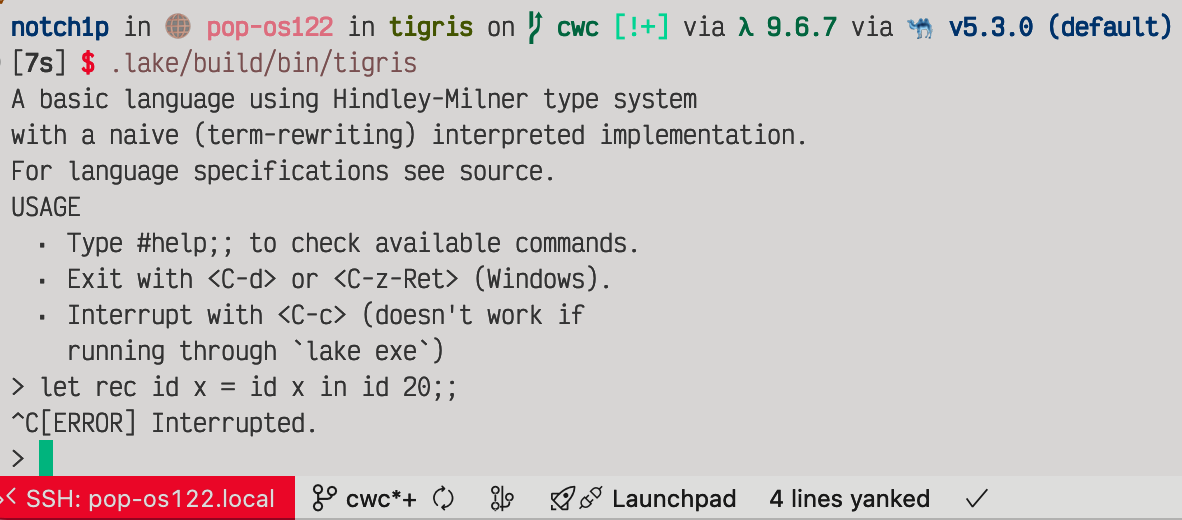
\includegraphics[width=0.38\linewidth]{assets/term1}
  \caption{某用户终止一次计算}\label{img:term1}
  \vspace{-1em}
\end{wrapfigure}
我们通过在解释器的热点分支之前做线程终止检测，以回应来自用户的线程终止信号，并在收到信号的同时跳出函数，实现
线程的正常终止。而之所以能够通过 CLI 前端按快捷键终止线程，是程序通过 Lean 的 C FFI 初始化
POSIX SIGINT 管道，捕捉用户发出的中断信号并提供管道的读写方法实现的。同时，我们还在 Lean 侧设置
一\emph{哨兵线程}，不断读取管道值以检测信号是否发出，若发出则终止。
\begin{minted}[numbers=left,baselinestretch=1]{c}
typedef lean_obj_res OBJRES; static int32_t sig_pipe[2] = {-1, -1};
LEAN_EXPORT OBJRES lean_sigint_pipe() {
  struct sigaction sa;
  if (sig_pipe[0] != -1) return lean_io_result_mk_ok(lean_box(sig_pipe[0]));
  if (pipe(sig_pipe) != 0)
    return lean_mk_io_user_error(lean_mk_string(/* ..错误信息.. */));
  memset(&sa, 0, sizeof(sa)); sa.sa_handler = sigint_handler;
  sigemptyset(&sa.sa_mask); sa.sa_flags = SA_RESTART;
  if (sigaction(SIGINT, &sa, NULL) != 0) {
    close(sig_pipe[0]); close(sig_pipe[1]);
    sig_pipe[0] = sig_pipe[1] = -1;
    return lean_mk_io_user_error(lean_mk_string(/* ..错误信息.. */)); }
  return lean_io_result_mk_ok(lean_box(sig_pipe[0])); }
\end{minted}
而这整套机制，由状态 \texttt{EvalState} 记录，
\begin{minted}[numbers=left,baselinestretch=1]{lean4}
abbrev EvalState := Option $ Task $ Except Error 
                  $ REPLState × LInterpreter.Val × Scheme
\end{minted}
其中 \texttt{Task} 是 Lean 原生类型，表示异步计算，与协程（coroutine）相仿，例如 Scala 的 \texttt{Future}，JS 的 \texttt{Promise} 和 Rust 的 \texttt{JoinHandle}.
总的来说，\emph{Tigrisi} 的实现是多方努力的成果：Lean 侧与 C 侧通过 FFI 实现中断机制的底层；
REPL 前端与解释器协作实现用户输入、编译器前端处理与降级、解释器求值与输出、出错中断、手动中断这一循环。

现在，若某程序不停机或运算时间过长，例如 \mintinline{ocaml}|let rec loop x = loop x in loop ()|，用户
即可通过快捷键 \texttt{<C-c>} 终止对应线程，如图 \ref{img:term1} 所展示的那样。
\emph{Tigrisi} 的主要功用并非
运行程序，而是方便开发者能够快速判断编译器的 IR 降级阶段是否实现出错。

\section{CPS 化}
\paragraph{CPS\upcite{reynolds1972definitional,sussman1998scheme} 变换} 亦称 CPS 化，指将 \Lambdair 转变为 CPS 风格 IR 的变换过程。以我们的实现为例，
CPS 变换后的 IR 具备以下特征：
所有函数接受一显式续点参数 $k$；
函数调用返回的结果应当传给续点，而非直接返回；
续点\emph{并非}头等公民，必须通过本地绑定产生，或上述的续点参数 $k$. 任一函数
从不能独立返回续点本身；
前述的 ANF 特征仍保留。

在尾调用优化一节我们曾提到过 CPS 可以用于将非尾调用函数变换成尾调用——这实际上是一个很具体且片面的说法。
全面地说，机械化（即编译器所作的，而非程序员手动的）的 CPS 变换的目的是\underline{编码复杂控制流}，
类似 C 语言的 \texttt{longjmp}. CPS 变换能够以堆空间为代价，显式化控制流交接，因为续点通常
以 lambda 编码\footnote{
  后者主要在堆上分配。虽然大多数编译器也会将其优化成栈上分配，如果条件允许——虽然这么做
  相当于抵消了用 CPS 来节约栈空间的目的。
}，并与其他参数一起在函数间相互传递。一言以蔽之，
CPS 通过在堆上复合续点，以堆空间换取栈空间。而复合而成的“大续点”则可以看作一个能够
替代调用栈但位于堆上的\emph{续点栈}，后者在被应用时会（在思想上）不断出栈，释放堆空间。

CPS IR 在定义上与 \Lambdair 相仿，但为了满足续点传递风格的需求新增、修改了一些语言构件。
在尾调用 \texttt{CTail} 中，我们增加新的构造子用于表示 CPS 风格的函数应用（\texttt{appFun}），
与续点应用（\texttt{appKont}），后者在 Reynolds 的论文中又称为 APPLY 操作；统一了
立即数与右手侧，统称 \texttt{CRhs}；并在表达式 \texttt{CExpr} 中统一了不同种类的 Let-绑定，
同时新增了专门用于绑定续点的 \texttt{letKont} 构造子。而相较于 \texttt{LFun}，\texttt{CFun}
用于表示 CPS 下的函数，自然也新增了一个栏位 \texttt{kontParam} 用于记录续点参数 $k$.
此外，我们还引入一个新的指令 \texttt{halt}，但并不常用——因为在 SBCL 下程序运行完不会终止，
控制权交移 SBCL，我们可以在此基础上继续编写 LISP 代码并使用 \Tigris 程序的计算结果。

CPS 变换是 IR 降级的最后一步，此后将由 SBCL 后端直接降级到 Common Lisp.
在不考虑后端的情况下，编译产物的程序的语义与 CPS IR 的语义应该一致。
为了能够使用 CPS IR 考察 \Tigris 的操作性语义，
我们下面给出 CPS 变换的指称语义\footnote{
  对于不熟悉 PLT 的用户来说，可以将这一步看成是 CPS 变换的变换法则，指导着
  具体实现。
}，与 CPS IR 自身的指称语义。首先给出 \Lambdair、CPS IR 的形式文法。
\begingroup\allowdisplaybreaks\setlength{\abovedisplayskip}{3pt}\setlength{\belowdisplayskip}{3pt}
%\begin{align*}
%\end{align*}
\begin{equation}\label{eq:lambda-cps-formal}
  \begin{aligned}
    v \in \Val &::= x \mid k \mid \ctor(t, \bar{x}) \mid \lambda p.\, e \\[4pt]
    r \in \mathsf{Rhs} &::= \prim(\mathit{op}, \bar{x}) \mid \proj(x, i) \mid \mkpair(x, y) \mid \mkctor(t, \bar{x}) \mid \isctor(x, t, n) \mid f(a) \\[4pt]
    s \in \mathsf{Stmt} &::= \letone x = r \\[4pt]
    \tau \in \mathsf{Tail} &::=\mathbf{ret}\, x \mid f(a)^{\mathsf{T}} \mid \fail \\
    &\mid \mathbf{if}\, c\, \mathbf{then}\, e_1\, \mathbf{else}\, e_2\\[-2pt]
    &\mid \switch^{\Const}(x, \overline{k_i \to e_i}, e_?) \\[-2pt]
    &\mid \switch^{\ctor}(x, \overline{(t_i, n_i) \to e_i}, e_?) \\[4pt]
    e \in \mathsf{LExpr} &::=\bar{s};\, \tau \mid \mathbf{let}_\iota\, x = v\, \mathbf{in}\, e
    \mid \letone x = r\, \mathbf{in}\, e\\
    &\mid \letRec\, \overline{f_i(p_i) = e_i}\, \mathbf{in}\, e\\[4pt]
    r_c \in \mathsf{CRhs} &::=\prim(\mathit{op}, \bar{x}) \mid \proj(x, i) \mid \mkpair(x, y) \mid \mkctor(t, \bar{x}) \mid \isctor(x, t, n) \mid k \mid x\\[4pt]
    e_c \in \mathsf{CExpr} &::=\mathsf{tail}\, \tau_c
    \mid\letone x = r_c\, \mathbf{in}\, e_c
    \mid \letK\, \kappa(p) = e_c\, \mathbf{in}\, e_c\\
    &\mid \letRec\, \overline{f_i(p_i, k_i) = e_i}\, \mathbf{in}\, e_c\\[4pt]
    \tau_c \in \mathsf{CTail} &::=f(p, k) \mid k(v) \mid \halt(v)
    \mid \fail\\
    &\mid  \ite(c, e_1, e_2) \\[-2pt]
    &\mid \switch^{\Const}(x, \overline{k_i \to e_i}, e_?) \\[-2pt]
    &\mid \switch^{\ctor}(x, \overline{(t_i, n_i) \to e_i}, e_?)
  \end{aligned}
\end{equation}
并定义语义域（domain of semantics，可看作数据类型）为，\footnote{
  $(+)$ 和 $(\times)$ 即分别为上文介绍过的 categorical product/coproduct.
}
\endgroup
\begingroup
\setlength{\abovedisplayskip}{3pt}\setlength{\belowdisplayskip}{3pt}
\begin{equation}\label{eq:cps-sem-domain}
  \begin{aligned}
    \Val &= \unit + \mathsf{Int} + \mathsf{Bool} + \mathsf{String} + (\Val \times \Val) + (\Name \times \Val^*) + \Name \\
    \Env &= \Name \rightharpoonup \Val \\
    \FunTab &= \Name \rightharpoonup (\Name \times \Name \times \mathsf{CExpr}) \\
    \KontTab &= \Name \rightharpoonup (\Name \times \mathsf{CExpr}) \\
    \mathsf{Ans} &= \Val + \mathsf{Error}
  \end{aligned}
\end{equation}
\endgroup
变换法则 $\mathcal{C} :  \mathsf{LExpr} \to \mathsf{CExpr}$ 是在给定\emph{当前续点} $k$ 下
定义的，$k$ 应当是一个指代续点的变量，或恒等续点（函数）$\mathrm{id}_\mathsf{Ans}$，
后者仅限于顶层，且为 SBCL 后端的标准入口点。

下面，我们给出这一变换的指称语义。注意 $\mathcal{C}^k_{[\bullet]}$ 表示 $k$ 绑定的、挖空的变换法则，下标的空
表示输入域元素 $[\bullet]$，为以下之一：$v, r, s, \tau, e$，而 $\mathcal{C}^k_s\sem{\bullet}(e_c)$ 携带（thread）$e_c$.
此外，我们简单化 \texttt{let*}、\texttt{switch*} 为单绑定/匹配对象，可类推多个。
\begingroup\setlength{\abovedisplayskip}{3pt}\setlength{\belowdisplayskip}{3pt}
\allowdisplaybreaks
\begin{align*}
  \mathcal{C}_v\sem{x} &= x \tag{Values} \\
  \mathcal{C}_v\sem{k} &= \mathsf{const}(k) \\
  \mathcal{C}_v\sem{\ctor(t, \bar{x})} &= \mkctor(t, \bar{x})\\
  \mathcal{C}_r\sem{\prim(\mathit{op}, \bar{x})} &= \prim(\mathit{op}, \bar{x}) \tag{Rhs} \\
  \mathcal{C}_r\sem{\proj(x, i)} &= \proj(x, i) \\
  \mathcal{C}_r\sem{\mkpair(x, y)} &= \mkpair(x, y) \\
  \mathcal{C}_r\sem{\mkctor(t, \bar{x})} &= \mkctor(t, \bar{x}) \\
  \mathcal{C}_r\sem{\isctor(x, t, n)} &= \isctor(x, t, n) \\
  \mathcal{C}_r\sem{f(a)} &= \text{（见下方函数调用变换）}\\
  \mathcal{C}_\tau^k\sem{\mathbf{ret}\, x} &= \mathsf{tail}\, k(x) \tag{Tails} \\[6pt]
  \mathcal{C}_\tau^k\sem{f(a)^{\mathsf{T}}} &= \mathsf{tail}\, f(a, k) \\[6pt]
  \mathcal{C}_\tau^k\sem{\mathbf{if}\, c\, \mathbf{then}\, e_1\, \mathbf{else}\, e_2} &=
  \mathsf{tail}\, \ite(c, \mathcal{C}^k\sem{e_1}, \mathcal{C}^k\sem{e_2}) \\[6pt]
  \mathcal{C}_\tau^k\sem{\switch^{\Const}(x, \overline{k_i \to e_i}, e_?)} &=
  \mathsf{tail}\, \switch^{\Const}(x, \overline{k_i \to \mathcal{C}^k\sem{e_i}}, \mathcal{C}^k\sem{e_?}) \\[6pt]
  \mathcal{C}_\tau^k\sem{\switch^{\ctor}(x, \overline{(t_i, n_i) \to e_i}, e_?)} &=
  \mathsf{tail}\, \switch^{\ctor}(x, \overline{(t_i, n_i) \to \mathcal{C}^k\sem{e_i}}, \mathcal{C}^k\sem{e_?}) \\[6pt]
  \mathcal{C}_\tau^k\sem{\fail} &= \mathsf{tail}\, \fail\\
  \mathcal{C}_s^k\sem{\bar{s};\, \tau} &= \mathcal{C}_s^k\sem{\bar{s}}(\mathcal{C}_\tau^k\sem{\tau}) \tag{Stmt} \\
  \mathcal{C}_s^k\sem{\epsilon}(e_c) &= e_c \\
  \mathcal{C}_s^k\sem{(\letone x = r); \bar{s}}(e_c) &=
  \begin{cases}
    \letK\, \kappa(x) = \mathcal{C}_s^k\sem{\bar{s}}(e_c)\, \mathbf{in}\, \mathsf{tail}\, f(a, \kappa)
    & r = f(a) \\
    \letone x = \mathcal{C}_r\sem{r}\, \mathbf{in}\, \mathcal{C}_s^k\sem{\bar{s}}(e_c)
    & \text{otherwise}
  \end{cases}\\
  \mathcal{C}^k\sem{\mathbf{let}_\iota\, x = v\, \mathbf{in}\, e} &=
  \letone x = \mathcal{C}_v\sem{v}\, \mathbf{in}\, \mathcal{C}^k\sem{e} \tag{letVal} \\
  \mathcal{C}^k\sem{\letone x = f(a)\, \mathbf{in}\, e} &=
  \letK\, \kappa(x) = \mathcal{C}^k\sem{e}\, \mathbf{in}\, \mathsf{tail}\, f(a, \kappa) \tag{letRhs} \\
  \mathcal{C}^k\sem{\letone x = r\, \mathbf{in}\, e} &=
  \letone x = \mathcal{C}_r\sem{r}\, \mathbf{in}\, \mathcal{C}^k\sem{e}
  \quad (r \neq f(a)) \\
  \mathcal{C}^k\sem{\letRec\, f(p) = e_f\, \mathbf{in}\, e} &=
  \letRec\, f(p, k_f) = \mathcal{C}^{k_f}\sem{e_f}\, \mathbf{in}\, \mathcal{C}^k\sem{e} \tag{letRhs}
\end{align*}
\endgroup
最后，我们给出 CPS IR 本身的指称语义，由以下两变换给定：
\begingroup
\begin{equation}
  \begin{aligned}
    \mathcal{E} &: (\mathsf{CExpr}\oplus\mathsf{CTail}) \to \Env \to \FunTab \to \KontTab \to (\Val \to \mathsf{Ans}) \to \mathsf{Ans}\\
    \mathcal{R} &: \mathsf{CExpr}\to\Env\to\Val
  \end{aligned}
\end{equation}
\endgroup
其中第五个参数 $\Val\to\Ans$ 是外层（顶层）续点 $\mu$，亦称元续点（metacontinuation），表示
能够使该续点层级的函数返回（无论有多深）。
记 $\rho[n\mapsto v]$ 为绑定（映射）$n\mapsto v$ 到 $\rho$ 的插入操作，
具有如下语义：若键 $m$ 存在及其对应值存在，用值 $v$ 替换之。注意此处所用 $\rho,n,v$ 都是元变量；
$\mathcal{E}$ 接受一 sum/coproduct type $\mathsf{CExpr}\oplus\mathsf{CTail}$，
表示这一参数既可以是尾调用 $\mathsf{CExpr}$，也可以是表达式 $\mathsf{CTail}$.
\begingroup\allowdisplaybreaks
\begin{align*}
  \footnotemark\mathcal{R}\sem{\prim(\mathit{op}, \bar{x})}\Env &= \delta(\mathit{op}, \Env(\bar{x})) \tag{CRhs} \\
  \mathcal{R}\sem{\proj(x, i)}\Env &= \pi_i(\Env(x)) \\
  \mathcal{R}\sem{\mkpair(x, y)}\Env &= (\Env(x), \Env(y)) \\
  \mathcal{R}\sem{\mkctor(t, \bar{x})}\Env &= (t, \Env(\bar{x})) \\
  \mathcal{R}\sem{\isctor(x, t, n)}\Env &=
  \begin{cases}
    \mathsf{true} & \Env(x) = (t, \bar{v}) \land |\bar{v}| = n \\
    \mathsf{false} & \text{otherwise}
  \end{cases} \\
  \mathcal{R}\sem{\mathsf{const}(k)}\Env &= k \\
  \mathcal{R}\sem{\mathsf{alias}(y)}\Env &= \Env(y)\\
  \mathcal{E}\sem{f(p, k)}\Env\FunTab\KontTab\mu &=
  \begin{cases}
    \mathcal{E}\sem{e_f}\Env'\FunTab'\KontTab'\mu
    & \FunTab(f) = (p_f, k_f, e_f) \tag{funapp} \\
    \mathsf{Error} & \text{otherwise}
  \end{cases}\\
  \text{where}\quad\Env' &= \{p_f \mapsto \Env(p),\, k_f \mapsto \Env(k)\}, \\[-4pt]
  \FunTab' &= \FunTab, \KontTab' = \varnothing \quad \text{（本地绑定的续点不逸出）}\\[-4pt]
  \footnotemark\mathcal{E}\sem{\kappa(v)}\Env\FunTab\KontTab\mu &=
  \begin{cases}
    \mathcal{E}\sem{e_\kappa}\Env[p_\kappa \mapsto \Env(v)]\FunTab\KontTab\mu
    & \KontTab(\kappa) = (p_\kappa, e_\kappa) \tag{kontapp} \\
    \mu(\Env(v))
    & \kappa = k_{\mathsf{param}} \\
    \mathsf{Error} & \text{otherwise}
  \end{cases}\\
  \mathcal{E}\sem{\halt(v)}\Env\FunTab\KontTab\mu &= \Env(v) \tag{halt}\\
  \mathcal{E}\sem{\ite(c, e_1, e_2)}\Env\FunTab\KontTab\mu &=
  \begin{cases}
    \mathcal{E}\sem{e_1}\Env\FunTab\KontTab\mu & \Env(c) = \mathsf{true} \tag{conditional} \\
    \mathcal{E}\sem{e_2}\Env\FunTab\KontTab\mu & \text{otherwise}
  \end{cases}\\
  \mathcal{E}\sem{\switch^{\Const}(x, \overline{k_i \to e_i}, e_?)}\Env\FunTab\KontTab\mu &=
  \begin{cases}
    \mathcal{E}\sem{e_j}\Env\FunTab\KontTab\mu
    & \exists j.\, \Env(x) = k_j \tag{const switch} \\
    \mathcal{E}\sem{e_? }\Env\FunTab\KontTab\mu
    & \forall i.\, \Env(x) \neq k_i \land e_? \ \text{exists} \\
    \mathsf{Error} & \text{otherwise}
  \end{cases}\\
  \mathcal{E}\sem{\switch^{\ctor}(x, \overline{(t_i, n_i) \to e_i}, e_?)}\Env\FunTab\KontTab\mu &=
  \begin{cases}
    \mathcal{E}\sem{e_j}\Env\FunTab\KontTab\mu
    & \Env(x) = (t_j, \bar{v}) \land |\bar{v}| = n_j \tag{ctor switch} \\
    \mathcal{E}\sem{e_?}\Env\FunTab\KontTab\mu
    & \text{no match}; e_?\ \text{exists} \\
    \mathsf{Error} & \text{otherwise}
  \end{cases}\\
  \mathcal{E}\sem{\fail}\Env\FunTab\KontTab\mu &= \texttt{MATCH-FAILURE} \tag{matchfail}\\
  \mathcal{E}\sem{\letone x = r\, \mathbf{in}\, e}\Env\FunTab\KontTab\mu &=
  \mathcal{E}\sem{e}\Env[x \mapsto \mathcal{R}\sem{r}\Env]\FunTab\KontTab\mu \tag{let1}\\
  \footnotemark\mathcal{E}\sem{\letK\, \kappa(p) = e_\kappa\, \mathbf{in}\, e}\Env\FunTab\KontTab\mu &=
  \mathcal{E}\sem{e}\Env\FunTab\KontTab[\kappa \mapsto (p, e_\kappa)]\mu \tag{letKont}\\
  \mathcal{E}\sem{\letRec\, f(p, k_f) = e_f\, \mathbf{in}\, e}\Env\FunTab\KontTab\mu &=
  \mathcal{E}\sem{e}\Env\FunTab[f \mapsto (p, k_f, e_f)]\KontTab\mu \tag{letRec}\\
  \mathcal{E}\sem{\mathsf{tail}\, \tau}\Env\FunTab\KontTab\mu &=
  \mathcal{E}\sem{\tau}\Env\FunTab\KontTab\mu \tag{tail}
\end{align*}
\endgroup
受过训练的读者可以立马反应出上述 CPS IR 的一些特征，我们列在下面。

\addtocounter{footnote}{-2}
\footnotetext{$\delta$ 指原生操作；$\pi_i$ 指投影。}
\stepcounter{footnote}
\footnotetext{情况二处理顶层续点 $\mu$，相当于从当前函数返回。}
\stepcounter{footnote}
\footnotetext{注意续点自身不构成值（是二等公民）；续点由单独的续点表 $\KontTab$ 记录。}

\begin{remark}[二等公民续点] 指在本 IR 中续点只能出现在下列语法位置：
  在函数调用的第二个参数上 $f(p, k)$；
  在续点应用中 $\kappa(v)$；
  由 $\letK\, \kappa(p) = e\, \mathbf{in}\, \ldots$ 绑定
  这一性质由 CPS IR 的定义保证，因为 \texttt{CRhs} 根本不含续点（也就是说，本 CPS IR 不能返回续点）。

  有一些读者可能感到失望，因为他们发现这样的 IR 不支持更高端的原生控制流操作，例如著名的 $\mathsf{call/cc}$ 和 delimited
  continuation\upcite{felleisen1988theory} 中的 $\mathsf{shift}$/$\mathsf{reset}$. 虽然必须承认将这些操作原生化以允许
  编译器对待之能获得更好的运行时性能，但 CPS 本身并非常用的编程风格，且以程序员心智负担代价换来的
  表达力是否值得亦是需要探讨并经过调查研究的问题。我们建议即便必须使用 CPS，也应考虑 \texttt{Monad} 接口提供的\emph{内化}（internalized）的 \texttt{Cont} 单子，
  最小化 CPS 在全局的影响，并提供更好的可维护性\footnote{
    从思考难度上讲，CPS 并不直观，且滥用之与 \texttt{goto} 无异。
  }，参照 \texttt{Control.Monad.Cont}.
\end{remark}

\begin{remark}[尾调用保证] 指 CPS IR 中的任一函数调用都在尾调用位置。
  在 \Lambdair 中的非尾调用是通过 $\letK$ 编码的：
  \begingroup\setlength{\abovedisplayskip}{5pt}\setlength{\belowdisplayskip}{5pt}
  \begin{equation}
    \letone x = f(a)\, \mathbf{in}\, e
    \quad\leadsto\quad
    \letK\, \kappa(x) = \mathcal{C}^k\sem{e}\, \mathbf{in}\, \mathsf{tail}\, f(a, \kappa)
  \end{equation}
  \endgroup
  其中续点 $\kappa$ 捕捉了\underline{程序的剩余部分} $e$.
\end{remark}
%\begin{remark}[CPS 变换后的闭包表示]
%  前文我们曾介绍过函数对象的编码与调用规范——这些标准在 CPS IR 中几乎一致。考虑
%  \(
%    \mathbf{C}\llbracket \mathit{ptr}, \Gamma \rrbracket
%  \)，
%  在 CPS IR 中，函数调用变为（$p$ 仍然是前文的 payload）
%  \[
%    \mathcal{E}\sem{f(p, k)} = \cdots\ \text{其中}\ f\ \text{是一函数指针}.
%  \]
%\end{remark}
%\begin{remark}[CPS IR 模块语义]
%虽然 \Tigris 没有提供任何的模块管理功能，但其已经具备一些先决条件，譬如 CPS 变换模块中已经定义了\emph{模块}——
%任一 \Tigris 源文件自动构成一个模块。CPS IR 的一个模块包含
%  \begin{equation}
%    \begin{aligned}
%      M = (\bar{F}, F_{\mathit{main}}) && F = (f, p, k, e)\\
%      \mathcal{M}\sem{(\bar{F}, F_{\mathit{main}})} =
%    \mathcal{E}\sem{e_{\mathit{main}}}\Env_0\FunTab_0\varnothing\,\mathrm{id}_\mathsf{Ans}
%    \end{aligned}
%  \end{equation}
%  其中
%  \begin{equation}
%    \begin{aligned}
%      \FunTab_0 &= \{f_i \mapsto (p_i, k_i, e_i) \mid F_i\ \mathbf{of}\ (f_i, p_i, k_i, \cdot) \in \bar{F}\} \cup \{f_{\mathit{main}} \mapsto (p_m, k_m, e_m)\} \\
%      \Env_0 &= \{p_m \mapsto (\unit, \mathbf{E}\llbracket\rrbracket)\}
%    \end{aligned}
%  \end{equation}
%  默认的初始 payload，即 main 函数的参数为 $(((), ()), \mathbf{E}\llbracket\rrbracket)$\footnote{
%    回忆，对参数为 $a$ 的 1-元函数，我们构造 $(a, ())$ 即便 $a = ()$.
%  }，这一默认值可以轻易修改。
%\end{remark}

\section{后端: Common Lisp (SBCL) 与 FFI}\label{sect:ffi}
在进行介绍之前，不妨通过对应的数据类型先回忆一下 \Tigris 实现的所有阶段。
\begin{align*}
  \text{\Tigris 源代码}
  \xrightarrow{\text{\textcircled{\tiny 1}}}\mathsf{Expr}
  \xrightarrow{\text{\textcircled{\tiny 2}}}\mathsf{TExpr}
  \xrightarrow{\text{\textcircled{\tiny 3}}}\mathsf{FExpr}
  \xrightarrow{\text{\textcircled{\tiny 4}}}\mathsf{LExpr}
  \xrightarrow{\text{\textcircled{\tiny 5}}}\mathsf{CExpr}
  \xrightarrow{\text{\textcircled{\tiny 6}}}\text{LISP source}\\
  \text{其中}
  \begin{matrix*}[l]
    &\text{\textcircled{\scriptsize 1}}:\text{词法、句法分析}
    &\text{\textcircled{\scriptsize 2}}:\text{类型检查}
    &\text{\textcircled{\scriptsize 3}}:\text{SysF IR 繁饰、实例解析}\\
    &\text{\textcircled{\scriptsize 4}}:\text{\Lambdair 降级}
    &\text{\textcircled{\scriptsize 5}}:\text{CPS 化}
    &\text{\textcircled{\scriptsize 6}}:\text{SBCL 目标代码生成}
  \end{matrix*}
\end{align*}

\paragraph{SBCL 后端} 直接将 CPS IR 翻译为 Common Lisp 目标代码。由于 SBCL 是动态类型的函数式语言，
且 LISP 家族的语言可以直接看作无类型\lambdacalc（untyped \textasciitilde, UTLC），
多态特殊化或大部分的类型信息都不必要且续点直接由 lambda 编码，不存在任何形式的\emph{去函数化}（defunctionalization）。
选择 Common Lisp 而不是其他语言（如 JS）的原因纯粹是笔者的个人偏好，因为其喜欢使用宏。
下面非正式地给出各语言构件的直接翻译。
\begingroup\setlength{\parskip}{-.5em}
\subparagraph*{顶层函数} 指所有的函数（因为经过闭包转换）。函数 $fid(pl, k)$ 对应 \mintinline{lisp}|(defun fid (pl k))|.
\subparagraph*{Let/Kont 绑定与 kontapp} Let 绑定，即 \texttt{let1}，对应 \mintinline{lisp}|(let ((n v)) ..)|；
Kont 绑定指续点绑定，形如 \texttt{letKont k v = ..}，对应 \mintinline{lisp}{(labels ((k (v) ..)) body)}；
kontapp 指续点应用，形如 \texttt{APPLY k v}，对应 \mintinline{lisp}|(funcall (the function k) v)|.
\subparagraph*{闭包与函数调用} 闭包形如 $\mathbf{C}\sem{ptr, \Gamma}$，对应 \mintinline{lisp}|#'ptr| 若 $ptr$ 为顶层或 LISP \texttt{label} 语句绑定，
否则按构造值直接存储；闭包环境 $\Gamma$ 即 $\mathbf{E}\sem{\bar{f}}$，对每一栏位 $f$，
\begin{itemize}\itemsep-.5em
  \item 直接存储之，若其为闭包（即上述构造值），
    \item 以 \mintinline{lisp}|#'f| 引用之，若 $f$ 为顶层或 LISP \texttt{label} 语句绑定，
  \item 否则直接存储之。
\end{itemize}

函数调用形如 $f(a, k)$，对应 \mintinline{lisp}|(funcall (the function f) ..)|，如 $f$ 是本地函数指针；或 \mintinline{lisp}|(funcall #'f ..)|，如 $f$ 为顶层或 LISP \texttt{label} 语句绑定。
可以看出，函数定义、调用的形式都是一一对应的，这也符合我们的直观认识。
\subparagraph*{条件表达式与 switch 语句} 条件表达式形如 $\ite(c,t,e)$，对应 \mintinline{lisp}|(if c t e)|；
构造子匹配，形如 $\isctor(x, tag, \cdot)$，对应 \mintinline{lisp}|(eq (car x) tag)|；
switch 语句，按构造子/常量，分为
\begin{itemize}\itemsep-.8em
  \item $\switch^{\Const}(x, \overline{k_i \to e_i}, e_?)$ 对应
    \mintinline{lisp}|(cond (((equal x k_i) e_i) .. (t e_?)) ..)|
  \item $\switch^{\ctor}(x, \overline{(t_i, n_i) \to e_i}, e_?)$ 对应
    \mintinline{lisp}|(cond (((eq x t_i) e_i) .. (t e_?)) ..)|
\end{itemize}
{\setlength{\parskip}{-1em}
  \subparagraph*{元组与构造值} 元组形如 $pr = (p, q)$，对应 \mintinline{lisp}|(cons p q)|，并通过标准的
  \mintinline{lisp}|(car pp)|、\mintinline{lisp}|(cdr pp)| 投影；构造值形如 $ctag\sem{\overline{fld}}$，对应
  \mintinline{lisp}|(cons tag (vector @fld))|\footnote{
    其中 \texttt{vector} 表示 \mintinline{lisp}|'simple-vector|，即 LISP 自带数据结构中最快的连续型数组。
  }，而其投影 $x_i$ 对应 \mintinline{lisp}|(svref (cdr x) i)|. 上述特殊构造子 $\mathbf{E}$、$\mathbf{C}$ 的值亦
按此翻译。}
\endgroup

此外，出现在 CPS IR 中的所有符号，根据 LISP 的语法用 \texttt{||} 保持大小写区别。符号即对应变量——小节 \ref{sbcl:cav} 曾提到过
因为类型信息已经擦除，我们只能通过按需收集\emph{形状}来缓解歧义问题：
任何变量的初始形状都是未知的，但随着翻译进行，有可能被精练为其他形状。
由于这一做法是函数层级的，没有考虑跨函数层级的精练，且没有解决根本问题即笔者的设计失误，所以最终只能够缓解问题。
如果要从根本上解决，就必须重构降级、CPS 化，使得类型信息在经过这些阶段后能传递到后端。
\paragraph{运行时系统} 指原生操作的实现、入口代码和底层异常定义，譬如字符串等号 \texttt{\%string=}
和 \texttt{MATCH-FAILURE} 条件\footnote{
  Common Lisp 有\emph{条件系统}，较之其他语言的异常系统更加强大且泛化，因为
  可以用这一系统编码各种控制流，甚至还可以用之实现一套续点机制。
}，
在底层分别通过 SBCL 的 \mintinline{lisp}{sb-kernel:%sp-string=} 和 \mintinline{lisp}{define-condition} 实现、定义。
  Common Lisp 针对不同的数据类型有各种各样的等号。为了减少 LISP 因为动态语言产生的 overhead，我们依照表 \ref{tab:lisp-eq} 针对不同类型使用各自最适合的等号。
  \begin{wraptable}{l}{4cm}\vspace{-.6cm}\centering\caption{LISP 等号}\label{tab:lisp-eq}
    \vspace{-.3cm}
    \footnotesize
    \begin{tabular}{@{}ll@{}}
      \toprule
      \textbf{对象} & \textbf{等号}                               \\ \midrule
      Symbols/NIL/T               & \texttt{EQ}                                         \\
      Precise numbers               & \texttt{EQL}                                        \\
      Cons/String                 & \texttt{EQUAL}                                      \\ \bottomrule
    \end{tabular}
    \vspace{-.6cm}
  \end{wraptable}
  \texttt{EQ} 是物理等号，而非结构等号，即它
  比较内存地址，因而速度最快。例如在 Lean 中，构造子由整数编码，比较构造子就是比较整数——
  因为 LISP 支持符号计算，在此处构造子就是符号，由于符号在 LISP 中唯一，我们用 \texttt{EQ} 比较其
  内存地址最快，媲美 Lean 在这一步的性能。

  \paragraph{FFI} 即外部函数接口，指用于调用外部函数的语言机制。因为我们编译到 SBCL，一个
  既高层又底层的语言\footnote{
    Common Lisp 的高层在于其有垃圾回收内存管理（GC），是动态类型语言；
    其底层在于有许多可与 C 媲美且更底层的控制流操作符，例如
    \mintinline{lisp}{go}、\mintinline{lisp}{block}、\mintinline{lisp}{progn}，其历史可
    追溯到上世纪五十年代。
  }，FFI 机制已经自动成型，只要用户清楚上文介绍的函数调用规范即可。这是因为我们不必关心内存管理问题，
  或是值的 boxing/unboxing 问题\footnote{即决定一个值是立即数还是通过指针引用的问题。此处的指针就是底层的内存指针。}。
  此外，我们还活用 LISP 的元编程能力，化简 FFI 函数的定义过程，方便用户使用。
  当然，因为 \Tigris 编译器看不见也看不懂 FFI 函数的定义，因此其全盘信任用户，后者应\underline{确保 FFI 函数在 LISP 侧的名字正确、具有正确的类型声明}。

  显然，以这种方式声明的类型签名（模式）没有办法检查其正确性，也就是说，可以
  引入一些类型明显为空的值，或者那些只有通过循环论证（不停机递归函数）才能证明的类型，
  例如 $\forall\alpha.\;\alpha$ 或 $\forall\alpha,\beta.\;\alpha\to\beta$.
  当然，后者并不是毫无用处。考虑一个特殊化的版本 $\forall\alpha.\;\mathsf{Unit}\to\alpha$，
  在之后的一个例子中就能用上。
  此外，从证明论的角度考虑，一个外部函数声明其实就是一条\emph{公理}——因为我们直接声明某一个类型存在值，
  却不给出证明——这就是公理化（axiomatic）的。

  下面以一个稍复杂的例子说明 FFI 的设计和使用。首先利用 FFI 声明引入数个外部函数 \texttt{println}、\texttt{toString}、\texttt{read}，
  用于对象字符串化、stdin 输入与 stdout 输出，
  同时通过用户自定义算符引入中缀左结合 \texttt{(++)}、前缀 \texttt{(!)} 算符并将之分别绑定为字符串连接和
  即将定义的阶乘函数，即

\begin{minted}[frame=single]{lean4}
extern println  "%println"   : forall a, a -> Unit
extern toString "%to-string" : forall a, a -> String
extern read     "%read"      : forall a, Unit -> a
infixl  65  "++" => append
postfix 50  "!"  => fact
\end{minted}
  以此可实现一简单程序：用户输入一整数，打印其阶乘值及阶乘的各步骤。
\begin{minted}[frame=single]{ocaml}
let fact n =
  let rec go acc
    | 0 => acc
    | m =>
      let _ = println
            $ "fact " ++ toString (n - m) ++ " = " ++ toString (acc * m)
      in go an @@ m - 1
  in go 1 n
let main =
  let _ = println "Enter a number:"
  and x = read () in x !
\end{minted}
  因为 \texttt{x!} 也是合法标识符，所以我们用空格隔开。
  此外，\texttt{read} 不安全，因为其应用值可被实例化到任意类型，此处为 \texttt{Int}.
  具体实现中，与 FFI 定义相关联的标识符在句法分析期间就被替换为字符串内的符号，例如
  \texttt{read} 到 \texttt{\%read}. 而这几个外部函数在 LISP 侧的实现极为简单；右侧给出输出结果。
  \begin{figure}[H]\centering
    \begin{subfigure}[c]{.65\textwidth}\centering
    \begin{minted}[frame=single]{lisp}
(defforeign "%string-append" (x y)
  (declare (ignore gamma) (type string x y))
  (funcall k (concatenate 'string x y)))
(defforeign |%read| (_ __)
  (declare (ignore gamma _ __))
  (funcall k (read)))
\end{minted}
    \end{subfigure}%
    \begin{subfigure}[c]{.35\textwidth}\centering
\begin{Verbatim}[baselinestretch=1]
$ ./dist-fact.fasl
  Enter a number:
  > 5           ; stdin
  fact 0 = 5    ; stdout
  (.. 略 ..)
  fact 4 = 120
\end{Verbatim}
    \end{subfigure}
  \end{figure}
  \texttt{defforeign} 是一自定义宏，活用 LISP 元编程功能简化 FFI 函数的定义，有语法\footnote{
    读者只需要理解为：宏 \mintinline{lisp}|(defforeign function-name (x y) forms)|
    声明并返回一闭包对象，其中 \texttt{(x y)} 是 \texttt{ffi-lambda-list}，表示
    声明的函数参数，长度不定；\texttt{forms} 表示由多个语句组成的函数体。
    此处依 LISP 惯例，使用与 X3J13/CLtL2 相同的 BNF 语法。
  }
  \begingroup\setlength{\abovedisplayskip}{3pt}\setlength{\belowdisplayskip}{3pt}
  \begin{equation}
    \mathbf{defforeign}\ \textit{function-name}\ \textit{ffi-lambda-list}\ \{\textit{form}\}^*\longrightarrow \textit{closure-object}
  \end{equation}
  \endgroup
  其本质上是 LISP 函数声明与全局变量声明的结合体。
\begin{minted}[numbers=left,baselinestretch=1]{lisp}
(let* ((ns     (name-to-string name))
       (fn-sym (intern (escape-bar ns)))
       (cell   (intern ns))
       (clos   (make-closure fn-sym)))
  `(eval-when (:compile-toplevel :load-toplevel :execute)
     (defun ,fn-sym (payload k) 
                    (with-args payload ,arg-list ,@body))
     (defparameter ,cell ,clos)))
\end{minted}
  通过宏的帮助，在 LISP 侧定义 \Tigris 的 FFI 函数就和定义普通 LISP 函数一般简单。
  \section{本章小结}
  本章从 \Lambdair 及其周边、CPS 化、SBCL 后端、运行时系统与 FFI 的顺序对 Tigris 编译器的中后部分的实现与设计进行叙述，
  与实现顺序、编译顺序一致。在实现上，本章是任务最为繁重的一个模块：其不仅代表着“编译”的字面义，
  更因为本章 \Lambdair 的设计失误而加重。
%\newpage
%\thispagestyle{empty}
%\null
\chapter{PP：\emph{依赖类型}的表格打印器}
本文倡导依赖类型编程实践，而最好的倡导方式就是讲解实例。各种实例中，又以
那些具有工程价值，被实际运用于项目中的为贵。因而，我们专门用一章来介绍 \Tigris 实践中使用的
依赖类型编程，以此作为范例，并承上启下，令读者熟悉何为依赖类型，为下一部分的定理证明子系统 \Tigrisd 叙述奠基。

实际上，\Tigris 使用的依赖类型完全不止本节的标题，还包括一些（互）递归函数的停机证明，但下文
以叙述 PP 打印器的设计与实现为主，并以此展示依赖类型论如何能帮我们在编译期发现更多的程序错误，
并为读者提供依赖类型方法论的基本认识。

PP 打印器自身，被广泛运用于命令行信息的\emph{美观输出}，例如
\Tigris 的 REPL 可以通过 \texttt{\#check} 命令打印类型环境表格；编译器 CLI 前端则可通过
\texttt{-h, --help} 参数打印帮助信息表格。

\begin{analysis}
  表格，本质上来说无非是一\emph{矩阵}。各种表格因为其承载数据的不同，即\emph{表头}的不同而不同。例如，
  表头（姓名、性别、年龄）显然和表头（产品名称、制造商、序列号、定价）指代的表格在意义上不同。然而，
  我们如何在语言中自然的区分两者——一种想法是利用类型检查器，只要能够区分两种表格的\emph{类型}即可，
  因此，我们转向依赖类型论的支持，PP 打印器由此而生。

  考虑作为 \texttt{List}（列表）的表头，可将其变换为\emph{动态长度}的元组，即
  使元组类型\emph{依赖于}表头长。这样，我们就要求该元组的类型与长度必须与表头一致，
  才能通过类型检查器。
\end{analysis}
由此，我们可以定义
\begin{minted}[numbers=left,frame=single]{lean4}
abbrev ToProd (as : List α) (m : Type -> Type) : Type :=
  match as with
  | [] => PUnit
  | [_] => mα
  | _ :: x :: xs => m α × ToProd (x :: xs) m
abbrev Row := ToProd header id
\end{minted}
%\begin{figure}[H]
%  \begin{subfigure}[c]{0.5\textwidth}
%  \end{subfigure}%
%  \begin{subfigure}[c]{0.5\textwidth}
%    \begin{align*}
%      &\mathsf{ToProd}\ (as : \mathsf{List}\ \alpha)\ (m : \mathbf{Type}\to\mathbf{Type}) =\\
%      &\quad
%      \begin{cases}
%        \mathsf{PUnit} &as = [];\\
%        m\ \alpha &as = [x];\\
%        m\ \alpha \times \mathsf{ToProd}\ (x :: xs)\ m &as = \cdot :: x :: xs.
%      \end{cases}\\
%      &\mathsf{Row}\ \textit{h} = \mathsf{ToProd}\ \textit{h}\ \mathrm{id}_\mathbf{Type}.
%    \end{align*}
%  \end{subfigure}
%  \caption{\texttt{ToProd} 在 Lean 中与数学中的定义比较}
%\end{figure}

上述定义可以理解为，$\mathsf{ToProd}\ (as : \mathsf{List}\ \alpha)\ f$ 可\emph{消去到} 1) $\mathsf{PUnit}$
泛类型宇宙的幺元 2) $f\ \alpha$ 或 3) $f\ \alpha \times \mathsf{ToProd}\ (\mathsf{cdr}\ as)\ f$，
根据 $as$ 的形状 1) 为空；2) 为单个类型；3) 包含两个及以上的类型。定理证明器术语中，称像这样
在\underline{项上做模式匹配并消去到\emph{不定}类型}的操作为 large elimination.

也就是说，\texttt{ToProd} 类型构造子（在此可看作类型上的函数）可以根据
$as$ 的\emph{值}（长度）\footnote{
准确地说，是 $2 + n$ 个类型之一，对长度为 $n$ 的 $as$.
}，消去到上述三个类型之一。可以发现，虽然我们是通过模式匹配实现这一变换的，
但为了和值上的编程做区分，称这种思考方式为基于\emph{消去子}（eliminator/recursor）的解读，且
该模式匹配在 Lean 的内核中也确实以消去子应用的形式存在。

\begin{remark}[motive]
\emph{Motive}（动机，定义中是 $m$）是类型论术语，表示消去的目标类型（或其一部分），可以理解为
函数式编程在数据结构中常用的 \texttt{map} 函数。而 \mintinline{lean4}{abbrev} 比起 \mintinline{lean4}{def}
又可保证上述定义是\emph{可消去的}（reducible），而非\emph{半消去}或\emph{不可消去}，这使得 Lean 的类型检查器
能够自动按需查看上述定义。
\end{remark}

\paragraph{表格行的定义} 现在规定，表格的一行（\texttt{Row}）由 \texttt{ToProd header id} 编码。这样，我们保证
某一表格必须与其表头的格式（形状）一致，保证不同表格可以根据表头区分，否则产生
类型检查器将报错。在此基础上，我们又可定义表格类型 \mintinline{lean4}{abbrev TableOf := Array (Row header)}.

注意，上述定义的类型 \texttt{Row}、\texttt{TableOf} 都是类型构造子，需要表头（\texttt{header}）作为参数传入。
之所以使用连续数组 \texttt{Array} 而非列表（链表）\texttt{List}，是因为前者性能更好。此外，虽然表格的列数由
表头固定，但表格的行数（条目数）显然是可以自由增长的，因而此处用动态数组编码是恰当的。

作为用户，表格打印器最重要的需求是\emph{美观}，最少也应当\emph{看起来像一个表格}。定义
\begin{minted}[numbers=left,frame=single]{lean4}
inductive Alignment | left | center | right
inductive PadsBy | perCell | perCol
abbrev Align := ToProd header λ _ => Alignment
abbrev OverrideWidth := ToProd header λ _ => Option Nat
\end{minted}
\texttt{Align} 和表头形状相同，表示每一列的对齐格式（左对齐、居中、右对齐）；
\texttt{PadsBy} 表示空白填充（padding）策略。\texttt{perCell} 要求所有格子具有相同宽度，且
该宽度由最大的格子决定；\texttt{perCol} 则与之类似，但单独为\emph{每列}按照其最大的格子设置宽度；
\texttt{OverrideWidth} 则能够给用户以细粒度的格子宽度控制，允许用户手动、独立设置每一列的
宽度。

除此之外，我们还定义了格子两侧的留白（margin）长度、截断开关，后者用于在输出时跳过零长度的格子。听起来很简单，
但使用恰当时能产生意想不到的作用，比如图 \ref{pp:comp} 通过结合两者实现缩进功能，用于打印编译器前端的帮助信息。
\begin{figure}[h]\centering
\begin{subfigure}{0.35\textwidth}\centering
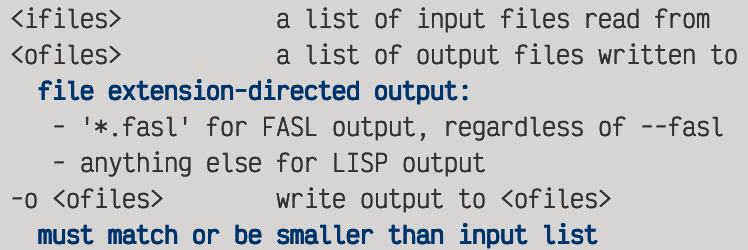
\includegraphics[width=\textwidth]{assets/term2}
\end{subfigure}%
\begin{subfigure}{0.65\textwidth}\centering
    \begin{minted}{lean4}
(.str "<ofiles>", .str "a list of input files read from")
(.str "", .byl "file extension-directed output:")
(.str "", .str " - '*.fasl' for FASL output ..")
(.str "", .str " - anything else for LIPS output")
    \end{minted}
\end{subfigure}
\caption{表格打印器的输出与对应的源代码条目}\label{pp:comp}
\end{figure}
\begin{figure}[htb]
\centering
%\begin{subfigure}{0.55\textwidth}\centering
%\begin{minted}{lean4}
%def ovTostr (ov : OverrideWidth header)
%  : String :=
%  match header with
%  | [] => "" | [_] => toString ov
%  | %[_, _ | _] =>
%    toString ov.1 ++ ovTostr ov.2
%\end{minted}
%\end{subfigure}%
%\begin{subfigure}{0.5\textwidth}\centering
%\begin{minted}{lean4}
%def zeroOverride (header : List Text.SString)
%  : OverrideWidth header :=
%  match header with
%  | [] => () | [_] => none
%  | %[_, y | ys] =>
%    (none, zeroOverride (y :: ys))
%\end{minted}
%\end{subfigure}\vspace{1em}
\begin{subfigure}{0.55\textwidth}\centering
\begin{minted}{lean4}
def maxN (h₁ h₂ : OverrideWidth header)
  : OverrideWidth header :=
  match header with
  | [] => () | [_] => max h₁ h₂
  | %[_, _ | _] =>
    (max h₁.1 h₂.1, maxN h₁.2 h₂.2)
\end{minted}
\end{subfigure}%
\begin{subfigure}{0.5\textwidth}\centering
\begin{minted}{lean4}
def merge (h₁ h₂ : OverrideWidth header)
  : OverrideWidth header :=
  match header with
  | [] => () | [_] => max h₁ h₂
  | %[_, _ | _] =>
    (h₂.1 <|> h₁.1, merge h₁.2 h₂.2)
\end{minted}
\end{subfigure}\vspace{.5em}
\begin{subfigure}{\textwidth}\centering
%instance : ToString $ OverrideWidth header := ⟨ovTostr⟩
%instance : Zero     $ OverrideWidth header := ⟨zeroOverride header⟩
\begin{minted}{lean4}
instance : Max      $ OverrideWidth header := ⟨maxN⟩
instance : Union    $ OverrideWidth header := ⟨merge⟩
\end{minted}
\end{subfigure}
\caption{用于计算列宽的辅助函数及对应类型类实现}\label{code:pp-col}
\end{figure}

{\setlength{\parskip}{-1em}\paragraph{Discriminant Refinement} 基于这些类型定义，图 \ref{code:pp-col} 实现了一些辅助函数。我们以这些函数为引子，引入一个在后续的 \Tigrisd，或任何
依赖类型论语言中都十分重要的机制：\emph{被匹配对象的精练}（discriminant refinement）\footnote{
精练（refine）一词是类型论术语，指通过（用户提供的）类型环境内的信息，将一个\emph{较泛}的类型
中的一部分，或整体，变为更加具体的项的过程。
}。\texttt{ToProd}，
某种意义上可以看作一个“多态”的类型（长度不同，依赖表头形状）——但无论如何，其在同一时刻只能具有一个值（类型），
因为 Lean 是静态类型语言。那么，如何告诉编译器 \texttt{ToProd} 在\underline{何时具有何种类型}呢——我们就需要通过精练
被匹配对象来实现这点了。}

精练被匹配对象是类型论术语，其含义即为字面义，指模式矩阵可以用来精练（补充）被匹配对象的
类型信息。例如，\mintinline{lean4}{match h : x with | 0 => ...} 告诉编译器 \texttt{x} 在
模式矩阵的第一个分支下\underline{一定等于 0}（而不仅仅是 $x$ 具有类型 $\mathsf{Int}$），
并在类型环境中添加一条\emph{假设}（assumption）$h : x = 0$ 以供用户使用之——根据模式匹配的语义
这显然是正确的。这一技巧在依赖类型编程中极为常见，例如在此处我们通过三个分支\emph{指导}编译器 \texttt{ToProd} 应该
具有的具体形状：
\begin{enumerate}\itemsep0em
\item 模式 \texttt{[]} 指出 $\textit{header} = []$，根据定义，\texttt{ToProd} 只能是 $\mathsf{PUnit}$；
\item 模式 \texttt{[\_]} 指出 $\textit{header} = [\cdot]$，匹配单元素（类型为 $\alpha$）。由定义 \texttt{ToProd} 只能是 $f\ \alpha$；
\item 模式 \texttt{\%[\_, \_ | \_]}，是 \texttt{\_ :: \_ :: \_} 的语法糖，指出
$\textit{header} = \cdot :: (\cdot :: \cdot)$，匹配两个及以上元素。由定义 \texttt{ToProd} 只能是“动态”长度的元组。
\end{enumerate}

从前文模式匹配“是用于解构数据结构”的解读看来，这里的模式匹配毫无用处；这是因为此处的重点在于使用模式匹配进行\emph{分情况讨论}，
告诉类型检查器额外的信息，因为其自身没有能力（类型推断做不到）分三种情况进行讨论。如果删去模式匹配，
则会产生类型检查错误，因为 Lean 自身无法推断类型，且从证明的角度考虑，不分三种情况讨论也没有办法确定 \texttt{ToProd} 的具体类型。
上面的叙述看起来复杂，但其思想很简单：任何一个接触过中学数学，学习过分情况讨论的用户，其实都已熟悉一定程度上的依赖类型编程。读者只需知道
函数定义需要\emph{照抄}类型定义的形式（三种情况）即可。

\begin{remark}[Discriminant Refinement 的常见用途]
除上述用途之外，Discriminant Refinement 最为常见的用途就是向类型环境（证明环境）中
添加条件/假设。例如，列表上的 \texttt{foldr1} 通常不允许空列表，在 Haskell 中
将之应用于空列表会出现运行时错误。然而，在依赖类型编程语言中，如 Lean，我们只需
将这一要求作为条件 $h$ 引入即可，
\begin{minted}[frame=single]{lean4}
  def foldr1 (f : α -> α -> α) (as : List α) (h : as ≠ []) : α :=
    match as with
    | [] => h rfl |>.elim -- Lean 知道这条分支矛盾，删除也没问题
    | [x] => x
    | x :: y :: xs => f x (foldr1 f (y :: xs) nofun)
\end{minted}
其中，由参数位置引入的假设 $h$ 在第一分支内精练为 $[]\neq[]$，矛盾！因而我们手动证伪，并通过爆炸原理（ex falso）匹配结果类型 $\alpha$.
类似地，\texttt{nofun} 是一语法糖，要求 Lean 自动证明 $y :: xs \neq []$，这也是显然的：含有一个及以上元素的列表一定非空。
这样，一些在其他语言中需要约定俗成、口头要求的条件，在 Lean 中都可形式化，并被类型检查器所认识，从根本上（编译期）
杜绝一些语义错误。
\end{remark}

具有上述类型与辅助函数后，我们发现打印器的实现就相当简单了。由于篇幅所限，此处略过。

\section{本章小结}（..略..）

\vspace{1cm}

\begin{center}
\underline{\bf\Tigris 子系统的论述到此结束}。
\end{center}

%\newpage
%\thispagestyle{empty}
%\null
\chapter{\Tigrisd: 一个轻量定理证明器}
\renewottcommands[dd]

\Tigrisd 是一个试验性质、以依赖类型作为理论基础的定理证明器。\Tigris 与 \Tigrisd 一同，
构成了一套 PL(DI)/定理证明教育解决方案。\Tigrisd 在设计与实现上，
受到了 Lean、pi-forall、LambdaPi、elaboration-zoo 项目的深刻影响。

目前而言，\Tigrisd 使用 Haskell 实现，因其强壮、活跃的生态环境，拥有诸如 \texttt{Unbound} 等用于
操作\lambdacalc、AST 的库使得我们不必重新造轮子\footnote{
  相较而言，\Tigris 就是一个（几乎）全数独立实现的子系统。
  其中用到的许多函数、实现都是针对这一语言特化的，因而较难将之迁移到此处为 \Tigrisd 所用。
}。
虽然我们未来展望有一天能将之用 Lean 重写，并配套一个定理证明过（verified）的实现——重点是
当下已经拥有一个可以工作的原型。

在实现上，\Tigrisd 只包含四大部分：句法分析器、内核、命令行前端。
这一部分主要介绍内核的设计与实现，并提供一个简单的范例展示证明。

\paragraph{命名规范} “项（term）”一词，当单独使用时，包含常规语言（非依赖类型）中的\emph{类型}。
当“项”与“类型”一起使用时，大部分情况下前者不包括后者。“类型”永远指代类型，无论依赖与否。
“内核”一词可看作类型检查器的同义词。

\section{语言基础与基本概念}
\Tigrisd 所支持的语法与 \Tigris 极为相似，仅有少数例外，且都与前者作为依赖类型语言相关。
这一语法的实现仍然使用基于组合子的单子句法分析，其特殊之处在于 \emph{layout} 组合子，这一组合子
使用 off-side rules（缩进影响语义，如 Haskell）。这一例外是因为证明通常比程序更复杂，一些语法中的
连接词，如 \texttt{let..in} 中的 \texttt{in}，在依赖缩进的语法中可以省略，降低\emph{语法噪音}，
提升可读性。下面叙述重要语法构造的区别。

\paragraph{枚举族} 是前述代数数据类型的“升级版”。
\begin{definition}[枚举族声明] 由以下 BNF 给出
\begin{minted}{bnf}
<dtype-decl>    ::= inductive <dtype-name> <dtype-ibinder>* : Type
                    "where"? ("|" <dtype-branch>)*
<dtype-branch>  ::= <dtype-ctor> : sepBy1("->", <dtype-binder>)
<dtype-ctor>    ::= <upper-ident>
<dtype-name>    ::= <upper-ident>
<dtype-binder>  ::= <dtype-tbinder> | <dtype-ibinder>
<dtype-tbinder> ::= (<ident> : <term>)
<dtype-ibinder> ::= {<ident> : <term>}
\end{minted}
\end{definition}
例如一个将长度\emph{嵌入}类型的列表（换句话说，类型依赖长度）可定义为：
\begin{minted}[frame=single]{lean4}
inductive Vector (α : Type) (n : Nat) : Type where
  | Nil                                      where n = Zero
  | Cons {m : Nat} (x : α) (xs : Vector α m) where n = Succ m
\end{minted}
其中我们使用花括号 \texttt{\{\}} 表示类型无关（不参与编程计算）的绑定子。
构造子的结果类型将与定义类型做比较，确保两者的\emph{头}一致，在此处即 \texttt{Vector}.
这一声明显式地规定了两条约束，按分支分别为 $n = 0$ 与 $n = \mathsf{Succ}\ m$. 通过 \texttt{example} 关键字，
我们能引入匿名的定义用于测试这个类型的可用性：
\begin{minted}[frame=single]{lean4}
example: {α : Type} -> Vector α 0 := Nil
example: Vector Unit 2 := Cons 1 () (Cons 0 () Nil)
\end{minted}
\paragraph{函数} 定义现在有形式
\begin{definition}[函数定义] 由以下 BNF 给出
\begin{minted}{bnf}
<tm-lam>      ::= fun <dtype-binder>+ => <tm>
<tm-toplevel> ::= def <ident> <dtype-binder>* : <tm> := <tm>
\end{minted}
\end{definition}
注意：\Tigris 中介绍的 pattern matching let 语法糖并不适用于此处。若想使用模式匹配，
必须通过 \mintinline{lean4}|fun pat => ...| 语法糖或以下最基本形式使用：
\begin{minted}[frame=single]{lean4}
def map {α β : Type} {n : Nat} (f : α -> β) (as : Vector α n)
  : Vector β n :=
  match as with
  | Nil         => Nil
  | Cons m x xs => Cons m (f x) (map {α} {β} {n} f xs)
\end{minted}

\Tigrisd 目前并不具备隐式变量推断（implicit inference）或隐式项合成（implicit synthesis），因而我们
要求用户提供所有绑定的参数，如上例所示。\Tigrisd 的类型检查器仅实现一简单的双向算法，只具备有限的
推断能力。
应当铭记下述 \Tigris 与 \Tigrisd 在函数定义上的差距，暨依赖类型论最显然的特征，
\begin{center}
  \underline{函数能接收\emph{类型}作为参数，就像其能接收值一样，因为\emph{类型也是项}}。
\end{center}
这一特性产生了一些在 \Tigris 中需要拓展类型系统（例如 skolems）才能实现的规则。考虑将第二个分支的右手侧递归应用 \texttt{map xs ..} 替换成
\texttt{xs}，使得整个式子成为 \texttt{Cons m (f x) xs}——检查器将立马报错，因为其需要证明 $\mathsf{Vector}\ \alpha\ n$、$\mathsf{Vector}\ \beta\ n$
相等，即证 $h : \alpha=\beta$.\footnote{
  依赖类型论的\emph{相等性}是一个极为重要的概念，我们将在下一节给出具体介绍。
}显然根据现有信息，不可能证出上述等式，因为等号两侧是随机选取的类型。

\paragraph{模式匹配与（依赖类型）元组消去} 已经被减少到以下两种语法形式：
\vspace{-.8em}
\begin{itemize}\itemsep-.5em
    \item \mintinline{lean4}|match e with ..| 只接受构造值模式；
    \item \mintinline{ocaml}|let (x, y) := a in b| 并非上述结构的语法糖，而是用于实现
    （依赖类型）元组消去的语法构造。
\end{itemize}
\vspace{-.8em}
关于上一部分提到过的 discriminant refinement，\Tigrisd 亦支持，我们将在后文介绍。

\paragraph{类型/证明无关性} 指的是类型、证明一定被擦除而不出现在最终的程序中的性质，因为
两者并没有运行时表示。显然，对于类型检查器来说，确保擦除正确，不意外擦除\emph{有意义的}值十分重要。
\emph{无关性}（irrelevance）一词指上述现象，但并非只有证明和类型是无关的，在下文我们还能看到其他的无关项。

\paragraph{模块} 与 \Tigris 一致。任一 \Tigrisd 源文件自动构成一模块，由源文件名作为模块名。此外，
我们也实现了类 Haskell 文件顶端的声明：通过 \mintinline{haskell}|module X where| 定义一个模块 $X$,
由顶端声明 \mintinline{lean4}|import M1,..,M2| 将 $M_1,\dots,M_i$ 引入当前模块。

\paragraph{内置证明} 是 \Tigrisd 内建的证明手段。共五种，前四种为原生构造，后一种为语法糖。

\texttt{sorry}（证明）：可用于证明任意命题，显然是不合理的。实际使用中，我们用此
来标记一个未完成的证明，方便之后补全，而不使得编译器报错。此命令的任一使用都会触发编译器的报警，
并使得其本身和与之相关的所有定义都被标记为\emph{不相关}。

\texttt{rfl}（证明）：为 reflexivity（自反性）的简写，可证明 $a = a$，对任意项 $a$. 可以说这是
所有等式命题的\emph{根证明}，因为更复杂的证明无非是将等式的任一一侧变换成另一侧，并通过自反性得证。\texttt{rfl}
远比其看起来的复杂：其支持 $\alpha$-等价 和 $\beta$-等价，即经过任意有限步 $\alpha$/$\beta$-变换的两个项
在 \texttt{rfl} 下直接相等。

\texttt{exfalso tm}（证明）：即爆炸原理。\texttt{exfalso} 接收一个证伪的项，
以此证明任意命题，或“构造”任意类型的一个值。在没有假设的前提下，若独立证出证伪的项，说明
系统不合理（unsound）。

\texttt{(|>)}（证明）：即等式重写。表达式 $h\triangleright e$ 在左手侧接受一等号类型 $a = b$ 的证明 $h$，
在右手侧要求 $e = a$，则可以证明 $b$.

\texttt{nomatch tm}（证明）：表示模式匹配 $tm$ 不存在任何分支，可以看作是另一种形态的爆炸原理。
给定空类型 \mintinline{lean4}|inductive Empty|，若 \Tigrisd 能证明其不含任何 introduction rule（构造子），
则模式匹配其值 $tm$ 时可用 \texttt{nomatch} 证明任意命题，如
\begin{minted}[frame=single]{lean4}
example (h : Empty) (C : Type) : C := nomatch h
\end{minted}
在实现上，这些命令基本被硬编码到核心代数 \mintinline{haskell}|Term| 中，且有定义

\begin{minted}[numbers=left]{haskell}
type Type = Term
data Term = Type0 {- 非直谓的类型宇宙 -} | {- .. 略 .. -}
  | Sorry {- sorry 证明 -} | Print {- show 命令 -} | Rfl {- rfl 证明 -}
  | Rw Term Term {- (|>) 证明 -} | Contra Term {- exfalso 证明 -}
\end{minted}
其中，我们还定义了别名 \mintinline{haskell}|Type| 并将之绑定到项（\mintinline{haskell}|Term|）上：从这里
也可看出依赖类型论的特点：类型也是项。此外，上面提到的 \texttt{nomatch tm} 证明则并非由硬编码得到，
而是在句法分析阶段直接解糖成为模式匹配 \mintinline{ocaml}|match tm with|，但其不含任何分支。

搭配 \texttt{Unbound} 库，可以轻松的为这一核心代数实现 \lambdacalc 中最为重要的两个操作：\emph{$\alpha$-相等}判断
与\emph{变量代换}。

\begin{Verbatim}[numbers=left,baselinestretch=1]
instance Unbound.Alpha Term where
  aeq' ctx a b = gaeq (strip a) (strip b) where
    gaeq = Unbound.gaeq ctx `on` from
instance Unbound.Subst Term Term where
  isvar (Var x) = Just (Unbound.SubstName x)
  isvar _       = Nothing
\end{Verbatim}

其中 \texttt{aeq} 即 $\alpha$-相等，\texttt{isvar} 则用于判断核心代数中哪些是可以用于代换的变量；\texttt{on} 中缀应用
可以看作是二元函数的复合算符。给定函数 $f : \beta\to\beta\to\beta,\, g:\alpha\to\beta$，$f\ \mathrm{on}\ g:\alpha\to\alpha\to\beta$ 是
$f$ 在 $g$ 上的投影。

\paragraph{类型宇宙} 亦称 level，在 \Tigrisd 中只有一个，且是\emph{非直谓的}，即 \mintinline{lean4}|Type : Type|，而非 \mintinline{lean4}{Type 1}，读作类型宇宙 \mintinline{lean4}{Type}，存在于自身中，或
\mintinline{lean4}{Type} 的类型还是 \mintinline{lean4}|Type|. 虽然单一宇宙的直觉类型论
（Martin-Löf/Intuitionistic Type Theory，MLTT. 依赖类型论的一种，但也可作为其别称）已由
Girard 证明不合理\footnote{
  我们并不细究其为何不合理，因为那是数学家的工作。读者只需知道其原因类似为什么 ZF 集合论中需要
  正则公理；否则会产生罗素式（Russell-style）的悖论。
}，我们仍然以之作为理论基础，因其简单性。此外，有界递归、停机/完备性检查在 \Tigrisd 中都不存在。

\section{\Tigrisd 内核的形式化描述与实现细节}
类似第二部分，下面我们给出 \Tigrisd 内核的形式化描述，但同时在每一要点中附带实现介绍。
由于类型亦属于项，所以我们不再区分类型系统和值，统归于核心代数下。
\allowdisplaybreaks
\paragraph{核心代数与类型环境} 由于篇幅所限，我们略过核心代数的叙述，读者应当能够直接从
下方的判断规则中得知。首先给出类型环境上的操作，

%\nonterms[0pt]{tm}
%\nonterms{context}

\drules[g]{$\Gamma$}{Context construction}{nil, cons}
项的类型判断规则为
\drules[t]{$\Gamma\vdash a : A$}{Typing}
{ var
  , refl
  , impred-univ
  , app
  , cast
  , pair
  , eq
  , exfalso
  , lambda
  , pi
  , sigma
  , letpair
  , let
  , subst
, exfalso}

其中 $\Pi/\Sigma$ 类型分别表示依赖积/余积（dependent product/coproduct）类型。
Product，如其形式，与箭头类型 $(\cdot\to\cdot)$ 极为相似，可以看作其“升级版”。
区别在于，现在我们为箭头左手侧（逆变位置）
增加了一个标识符（label），允许箭头右侧提及左侧，即结果类型依赖于参数。显然，依赖积可以用于编码
函数类型，且如果出现在类型层面，可以用于编码 $\forall$ binder ——依赖类型论“免费给予”我们一般语言
中的参数多态，且毫不费力。
同理，coproduct 的右手侧也可
依赖左手侧，可用于编码元组类型。这两个类型的叫法很多，例如前者亦称 dependent function type，后者
称 dependent sum type. 为了表述清晰，我们统一使用范畴论术语 product/coproduct.

我们略去一些常量（$\mathsf{Bool}$、$\mathsf{Unit}$）的规则，因为这些规则
与 \Tigris 一致。不相关项的类型规则同上，但另外给出：

\drules[t]{$\Gamma\vdash a : A$}{Irrelevant Typing}{elambda, eapp, epi}

\Tigrisd 的双向类型算法存在两个类型判断（judgement）：检查与推断。这两个判断在实现中对应两个
（互）递归的函数 \texttt{infer}、\texttt{check}. 显然，两者是互相依赖对方的。此外，对于
类型检查器来说，上述两个判断其实是两个\emph{模式}，对于不同的语法结构，我们采用不同的模式：
例如当其遇到 \rref{C-lambda} 时，是检查模式；遇到 \rref{I-app-nonwhnf} 时，是推断模式。
这两个模式分别用类型判断 $\Gamma\vdash a\Leftarrow A$、$\Gamma\vdash a\Rightarrow A$ 表示。显然，
如果这个系统是\emph{正确}的，则应当满足
{\setlength{\abovedisplayskip}{3pt}\setlength{\belowdisplayskip}{3pt}
  \begin{align*}
    \Gamma\vdash a : A\ \text{if}\ \Gamma\vdash a\Leftarrow (A : \mathbf{Type})\wedge
    \Gamma\vdash a : A\ \text{if}\ \Gamma\vdash a\Rightarrow A
  \end{align*}
}
汇总起来，我们针对两个模式给出对应的类型规则。
\drules[c]{$\Gamma\vdash a\Leftarrow A$}{type checking}
{ lambda
  , refl
  , pair
  , switch-mode
  ,exfalso, let
  , letpair-RL
  , letpair-LR
  , subst-l
  , subst-r
}
\drules[i]{$\Gamma\vdash a\Rightarrow A$}{type inference}
{ var
  , app-nonwhnf
  , impred-univ
  , pi
  , ascribe
  , sigma
  , let
  , eq
  , app
, subst}

\paragraph{相等性} 一些读者可能注意到上述推断规则中出现了定义性相等\footnote{
  在 MLTT 中也是判断性（类型规则见下文）相等；在单一宇宙 TT 中是类型上的相等。
}，例如 \rref{C-switch-mode, I-App}. 这是因为在类型作为项的类型检查中，
若要确认两个类型（变量）相等，可能需展开其定义并做一些计算才能确定——不妨先解决\emph{什么是相等}这一问题。

在各种类型论中，有诸多不同但又相关（甚至交叉）的
相等性（equalities），例如元相等（meta\textasciitilde）、定义性相等（definitional\textasciitilde）、判断性相等（judgemental\textasciitilde）、命题性相等（propositional\textasciitilde）、类型上的相等（typal\textasciitilde）。
这些相等性的区别与交叉体现了不同类型论建模“相等”这一概念的不同思路。下文主要介绍 \Tigrisd 的类型论涉及的前三个概念。

\subparagraph{元相等}指那些非内化于类型论的相等性。之所以称其“元”，是表示其存在于类型论之上（不是在
类型论中定义的），定义在\emph{元理论}（可理解为实现）中的特点。最明显的例子是，若两个项具有相同
\emph{形状}——AST 相等（syntactic equality，语法上相等）——则它们\emph{一定相等}，
\underline{无论类型论如何}——\emph{语法相等}就是元相等的一种，所有类型论都具备这一相等性。
同时，绝大多数类型论都以\lambdacalc 作为核心代数，因此元相等性也包括 \emph{$\alpha$-等价}\footnote{
  $\alpha$-equivalence 指出，形式语言中的两个式子（例如类型、项、命题、环境等）等价，若它们仅存在
  \underline{约束（绑定）变量名字上的不同}。
}。
在 \Tigrisd 中，
元相等恰为此二种，其中后者通过 \texttt{Unbound} 库实现。该库提供了用于替换、计算自由变量、生成崭新变量
等一系列\lambdacalc 上的操作，避免重新造轮子带来的不便，也使我们的实现经得起考验。
例如上述包含 $\alpha$-等价的元相等、自由变量的计算，在 \texttt{Unbound} 库中即为函数
\begin{minted}[numbers=left]{haskell}
aeq :: Alpha a => a -> a -> Bool -- 中缀算符 '==='
fv  :: ( Alpha a, Typeable b
       , Contravariant f, Applicative f) => (Name b -> f (Name b)) -> a -> f a
id x = Lam $ Unbound.bind x $ Var x -- 在源代码中构建一个 Tigrisd 中的恒等函数的 AST
id 'x' === id 'y' -- alpha-equiv: (\x -> x) === (\y -> y): >>> True.
\end{minted}
\subparagraph{定义性相等}可以看作元相等的“升级版”。
准确地说，定义性相等是定义在\emph{式子}上的\emph{等价关系}（注意：并非\emph{等于}关系！），
它指出两个式子是等价的，若其具有相同的\emph{含义}——显然，它蕴含元相等。

定义性相等是\emph{内涵的}（intensional），与另一逻辑概念\emph{外延}相对。
前者关注的重点在于某一对象的具体\emph{定义}，后者在于该对象的\emph{外在表现}，或\emph{行为}。以集合为例，
“小于 3 的正整数集”是一集合的\emph{内涵定义}，而 $\{1,2\}$ 是其唯一的\emph{外延表述}。
在类型论上，具有相同意义的式子是\emph{内涵相等}的。

之所以称其为“升级版”，是因为绝大多数类型论都会在其\emph{理论内}再定义\emph{显式定义性相等}，后者与元相等统称\emph{定义性相等}。
重点在于，\underline{这些理论是\emph{如何}在其内部定义上述等号的}——由此引伸出三种类型论上的等号：判断性相等、命题性相等、类型上的相等。需要注意的是，三种等号并不一定互斥，例如 \Tigrisd 就满足其中不止一种的等号。
读者不妨与 \Tigris 的类型系统作比较：为什么我们不谈它的相等性呢？显然，
这是因为传统语言的类型系统允许的类型过于简单，
或者说，任何非依赖类型论中存在的项（类型）都过于简单，仅靠元相等，即类型 AST 上的比较便可实现。

此外，\emph{元相等}是所有类型论具有的共性。为做区分，定义性相等一词有时特指显式定义性相等。

\subparagraph{判断性相等}是类型论中最基础的等号。正如其意，判断性相等是在类型论中直接作为
一条判断规则引入的，比如后文将介绍的 $\Gamma\vdash A = B$——\Tigrisd 类型论的等号就是判断性相等。
通常（也包括 \Tigrisd）这一等号就是常规意义上的等于，满足自反性、交换性、传递性——将满足这些性质的
判断性相等称为\emph{判断性等价}。

判断性相等虽然基本，但不代表其使用广泛。主流定理证明器，特别是以 CIC 作为理论基础的，例如 Lean，使用
命题相等性。

\subparagraph{命题相等}适用于两层（即区分类型和命题的）类型论。这一表述与 Curry-Howard 同构的“命题即类型”
表述不冲突：以 Lean 为例，所有的命题存在于类型宇宙（此处称命题宇宙）$\mathbf{Prop}$ 中，所有的类型存在于 $\mathbf{Type}\ u/\mathbf{Sort}\ (u+1)$（其中 $u$ 是宇宙层级）\footnote{
  满足 $\mathbf{Type}\ u\equiv\mathbf{Sort}\ (u+1)$，$\mathbf{Sort}\ 0\equiv \mathbf{Prop}$，
  $\mathbf{Sort}\ 1\equiv \mathbf{Type}$.
}
中。命题仍然是类型，但其基底集为 Subsingleton（次单元素集合），即含有\emph{最多 1 个}
元素的集合。在这一情况下，等式 $1 = 0$ 实际上是（命题）类型 $\mathsf{Eq}\ 1\ 0$，故而
称其命题相等：由命题编码的等号。之所以这样处理，原因是多方面的，但最显著的原因之一即是方便命题无关性的实现。

\subparagraph{类型上的相等}与命题相等类似：由类型编码的等号，例如 Cubical TT、HoTT（同伦类型论，homotopy\textasciitilde）
\footnote{
  虽然后者采用的是“命题为类型”（proposition as types）的解读，应当算作命题相等。
}抑或任意基于\emph{泛等公理}（univalent axiom）的类型论的路径等号。一般把这个
类型称为恒等类型（identity type）或相等类型（equality\textasciitilde），记作 $\mathsf{Id}_A(x, x')$，对
某 $(x, x' : A\times A)$. 由于恒等类型自身在不同类型论中具有不同表述，且其性质涉及到同伦理论、范畴和拓扑
理论的知识，如图 \ref{fig:id-intro}，超出本文范围，我们在此不表。
\begin{figure}\centering
  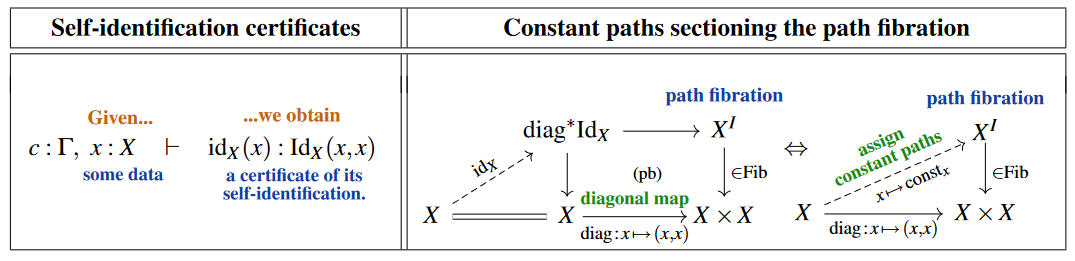
\includegraphics[scale=.9]{assets/MetaLogicOfIdentifications-1-220927.png}
  \caption{恒等类型的引入规则（introduction rule）在范畴论上的意义}\label{fig:id-intro}
\end{figure}

除此之外，类型上的相等在单一层级类型论中亦常见，根据 \rref{T-EQ} 可知，在 \Tigrisd 中，等号也是类型；同时，
我们摒弃恒等类型的记号，仍用等号，以强调其“相等”性。之所以要让相等成为类型，
是因为一个定理证明器最基本的需求，就是证明\emph{等式}命题：允许用户构造等式（类型）的证明（对象）。
然而，和 Lean 这样直接将等号作为命题构造出来的实现不同，我们直接将其内置在类型论中，故而，需要
以同样的方式引入类型上相等的规则——\rref{T-refl, T-eq, T-subst, T-exfalso} 分别给出了
等号的自反性、等号的组成规则（formation rule，可理解为类型层面上的 introduction rule）、
等号的重写规则（例如 $a = b$ 且 $b = 1$ 则 $a = 1$）和爆炸原理（从反面说就是反证法）。
此外，称同时具有判断性相等与类型上相等的类型论称为\emph{内涵类型论}。

上面说过，\Tigrisd 具有判断性相等。下面，我们引入其判断规则，并
搭配以类型规则，回答“何谓\emph{相等}”这一核心问题。

\drules[e]{$\Gamma\vdash A = B$}{Defintional/Judgemental equality}
{
  trans
  , subst-congr
  , beta
  , pi-congr
  , sigma-congr
  , app-congr
  , lam-congr
  , let-beta
  , let, refl, sym
  , pair-elim, var
  , pair-congr
  , typalsubst-beta
  , typalsubst-congr
  , typaleq-congr
}
%  , exfalso-congr
%  , eapp-congr
%  , elam-congr
%, epi-congr}

我们曾经说过，\underline{类型规则指导具体实现}——这一论断在此处仍然正确。然而，像上面这样的类型规则仅仅规范
具体行为，没有指出应当\emph{如何实现}。在 \Tigris 中，针对类型系统我们给出了\emph{具体实现}上的
类型规则；现在仿照前文，给出等号的具体实现规则，又称算法相等性（algorithmic\textasciitilde）。

在此之前，我们先介绍上面出现过的、等号实现所用到的重要概念：Weak Head 范式（WHNF）.

\paragraph{Weak Head Normal Form} 或前文出现的判断 $\Gamma\vdash\mathbf{WHNF}\ tm\leadsto nf$
读作：在环境 $\Gamma$ 下，$tm$ 化简为 WH 范式 $nf$.\footnote{
  这一概念因其与纯函数式语言的消去/求值策略相关，应当由 Peyton Jones（SPJ）提出。
}
首先，我们不妨回顾一下\emph{值}的定义。某一值为范式，当 $\langle v, \sigma\rangle\Downarrow\langle v\rangle$ 其中
$\sigma$ 表示一状态（若有）。在 \Tigrisd 中，值定义为

\nonterms{v}

WHNF 包括 $v$，且在其之上包含了更多的形式。其标准可以用一个词概括：\underline{不能再消去}的项。
除去\emph{值}，我们称 WHNF 包含的额外部分为\emph{中性项}（neutral term）。中性项主要包含
一系列嵌套的应用（application），且要求其头部为一\emph{变量}。虽然我们知道作为此变量的参数的
表达式可能是可消去的（redexes），但这一整体（应用）是不能的。因此，其属于 WHNF. 在 \Tigrisd 的核心代数中，
中性项包含

\nonterms{neutral}

例如，项 $(x : \mathbf{Type})\times (\lambda x.\,\mathsf{Nat})\ \mathsf{Unit}$ 是 WHNF.
虽然该类型的右手侧是 $\beta$-可消去的，式子整体则不行，因为其是一 coproduct type. 或者，考虑
中性项 $\mathsf{add}\ 1\ 3$：猜测应当消去到 $4$，但我们\emph{不能确定}这一猜测，因为没有看到/展开
$\mathsf{add}$ 的\emph{定义}，因而其也是 WHNF.

之所以引入 WHNF，是因为其关注\emph{消去策略}，亦称式子正规化——在实现等号时\emph{极为重要}，因为
我们希望相等性检查不只能处理最简单的情况（即形式一致的项），还应当支持一些\lambdacalc 的基本等价规则。
虽然一个简单的解释器能够通过完全消去（full reduction）支持那些等价规则，即一般意义上的求值，
但这还不够好，且存在潜在问题。因此，我们为项设置\emph{标准}，挑选不必立即消去的项来\emph{控制}消去策略——这就是 WHNF.

WHNF，具体的说，能够允许我们推迟\footnote{
  注意\emph{推迟}求值与\emph{惰性}求值之间的区别，一般来说后者包含前者。
}定义的展开，直到需要为止，即按需展开。这种消去策略在直觉上体现了符号计算
的思想；考虑等式 $f\ 3 = f\ (1 + 2)$ 其中 $f$ 表示某一冗长的计算。
等号两侧都是 WHNF，对于一个简单求值器来说，其会花费不必要的时间计算 $f$ 的应用，
但一个懂得 WHNF 的求值器可以直接比较 $3$ 和 $1 + 2$，因为两者具有相同\emph{头} $f$.
\emph{判定}这一等号也应当如此简单，因为我们完全不必展开 $f$.
而实际上，这不过是\emph{函数上的同余关系}（congruence relation）的特例。

然而，应当强调 \Tigrisd 的等号是半可判定的（semidecidable），因为等号的判定不一定停机——
我们没有保证定义的完备性。WHNF 能够\emph{缓解}这一问题，通过——如上所述——推迟定义展开：即便 $f$
不停机，上述等号仍然成立，且由证明器自动证出。当然，推迟不代表能避免，例如证明 $1 + 1 = 2$，
我们必须展开 $(+)$，且当 $(+)$ 不停机时，消去过程亦不停机，最终因为栈/堆空间耗尽而导致系统的崩溃。
不仅如此，我们还可以联系 Lean 的 \texttt{rfl} 或 Coq 的 \texttt{reflexivity} tactic：两者都要求
类型检查器开展正规化工作来判定相等性，且较之 \Tigrisd 更加强大，但实现类似，且目标都是尽量避免
立即求值。此外，作为编程语言来说，它们能够通过求值正规化（normalization-by-evaluation，NBE）直接
编译表达式到适合运行的形式，如 Coq 的 OCaml bytecode，达到接近普通程序运行的速度，加快证明器性能。

下面给出 WHNF 的消去规则（略去已经是 WHNF 的表达式）。

\drules[WHNF]{$\Gamma\vdash\mathbf{WHNF}\ a\leadsto nf$}{WHNF normalization}
{
  % var
  %, lam
  %  , pi
  %  , type
  lam-beta, let-beta
  , typalsubst-congr, letpair
  %  , def
  , prod-congr, typalsubst
  %  , typaleq-refl
  %  , refl
}

本文出现过许多类型规则，前面亦曾强调过，类型规则指导着实现——更确切的说，
类型规则在编程上给出了具体的实现步骤\footnote{从下往上读即可。这是类型规则，或者更广泛地说，证明树的特点。}。
譬如此处的 WHNF 消去，可以直接对应着写出具体代码——以 \rref{WHNF-letpair} 为例，我们撷取函数 \texttt{whnf} 的一部分如下所示
\begin{Verbatim}[numbers=left,baselinestretch=1]
whnf :: Term -> Bi Term
whnf (LetPair a b) = whnf a >>= \case
  Prod a₁ a₂ -> whnf $ instantiate b [a₁, a₂]
  e          -> return $ LetPair e b
whnf (Cond c t e) = whnf c >>= \case
  VB b -> if b then whnf t else whnf e
  c    -> return $ If c t e
\end{Verbatim}
这条规则及其对应实现告诉我们，若 WHNF 化后的绑定右手侧 $a$ \emph{确实是}元组 $(a_1, a_2)$，
则用后者代换 $b$ 中的 $x$ 和 $y$. 此外，我们还会发现 WHNF 化与常量折叠其实有部分重叠：如条件语句，
若条件已是一常量，则继续 WHNF 化 then-分支，否则 else-分支。

上述 WHNF 化工作，或更全面地说，\Tigrisd 的内核运行在 \texttt{Bi} 单子中，而这一单子的定义为
\begin{Verbatim}[numbers=left,baselinestretch=1]
type Bi = Unbound.FreshMT (ReaderT Env (EIO TypingError))
\end{Verbatim}

\texttt{Bi} 利用了 \texttt{Unbound} 所提供的 \texttt{FreshM}、\texttt{ReaderM} 转换器（名字以 \texttt{T} 结尾），保证引入的变量名唯一\footnote{
  Cf. \Tigris 的实现：我们存储了一个计数器以达到相同的作用。
}，
还携带了类型环境 \texttt{Env}，可以通过 \texttt{EIO}（具备错误处理的 IO 单子）向用户报告错误（\texttt{TypingError}）。
但必须要承认这一设计并不很“函数式”、不很“干净”。

\subparagraph{IO 的引入} 纯函数式编程鼓励传参、通过函数调用与返回实现数据的传递，同时将副作用局限在小范围函数中以方便程序员思考、维护程序。
输入/输出是显然的副作用，且与其他模拟副作用的“纯的”单子不同，因为其必须和外界（即操作系统交互），具备真正的副作用，因而其具有传染性：任何涉及到
IO 的函数自身必须在 IO 内：否则 IO 相关的函数返回的单子值就不能拿来使用——简单的说，
我们很容易（trivial）将一个函数抬进（lift）IO 中（$\alpha\to \mathsf{IO}\ \alpha$），但将任意 IO 包裹的值脱去 IO（$\mathsf{IO}\ \alpha\to\alpha$）则是困难的——
只能够在局部做到（即另一个 IO 内的函数体中），而不能在全局。
此处，输入输出副作用通过 \texttt{EIO} 单子引入——这说明整个内核都是都是\emph{不纯的}，即副作用发生在内核各处——这导致了可维护性问题：
我们无法精确地控制所有的副作用（以及其发生顺序），因为其散落在源代码各处，且程序运行逻辑的复杂性亦加重了这一负担。在 \Tigrisd 的内核中，
引入 IO 的主要目的是为了在出错时能够立马回报给用户（即输出到 stdout），但事后看来，一个更好的做法应当是维护一状态，用于收集内核检查过程中的所有（报错）信息，
保证内核实现的纯函数性，而对于内核产生的各种信息来说在内核结束后将之一一回报给用户更合适。
当然，考虑到目前的项目规模我们并未做这一改动，因为这会复杂化代码实现。

引入了 WHNF 后，我们便可以给出 \Tigrisd 的等号\emph{实现规则}。

\drules[impleq]{$\Gamma\vdash a \xlongequal{\mathsf{impl}} b$}{equality implementation}
{ refl
  , lam-congr
  , app-congr
  , pi-congr
, WHNF-ext}

这告诉我们 WHNF 的一个重要性质，即\underline{WHNF 化不改变两个式子的相等性}，或者说，
两个式子相等，当且仅当其 WHNF 相等。

\begin{proof}
  从左到右，由消去的不变性得证；反之，由 \rref{impleq-WHNF-ext} 规定。
\end{proof}

可以发现，等号的实现规则 $\Gamma\vdash a \xlongequal{\mathsf{impl}} b$ 相比描述等号性质的类型规则 $\Gamma\vdash A = B$ 要简单得多。
同理，将等号两侧 WHNF 后我们即可轻易地实现项在内核中的相等判定，由中缀算符 \texttt{(<=>)}、\texttt{impleq} 给定
撷取部分（变量、条件表达式、Let 绑定）如下。
\begin{Verbatim}[numbers=left,baselinestretch=1]
(<=>) :: Term -> Term -> FreshMT (ReaderT Env (Except TypingError)) ()
Var x <=> Var y | x == y = return ()
If c t e <=> If c' t' e' = c <=> c' *> t <=> t' *> e <=> e'
Let x b₁ <=> Let y b₂ =
  b₁ `fresh` b₂ >>= \(_, b₁, b₂) ->
    x <=> y *> b₁ <=> b₂
a <=> b | a === b = return ()

impleq :: Term -> Term -> Bi ()
impleq a b = do a <- whnf a; b <- whnf b; liftBi $ a <=> b
\end{Verbatim}
这里，我们吸取了 WHNF 中的教训，将 IO 副作用与等号判断分开，提升可维护性。因而仍需定义
一自然变换 \texttt{liftBi} 将不含 IO 的 \texttt{Bi} 提升回来，
\begin{Verbatim}[numbers=left,baselinestretch=1]
liftBi :: FreshMT (ReaderT Env (Except TypingError)) ~> Bi
liftBi (FreshMT{unFreshMT = act}) = FreshMT $
  StateT \st -> ReaderT $
    \rst ->
      case runExcept $ runReaderT (runStateT act st) rst of
        Left e -> throwError e
        Right x -> return x
\end{Verbatim}

\section{Discriminant Refinement}
上一部分说过，Discriminant Refinement 实现了证明中的\emph{分情况讨论}思考方式。
现在对此做一全面的叙述。我们假设读者已经阅读了上一部分，并对之有基本了解。

在许多定理证明器，例如 Lean 和 \Tigrisd 中，用户可以通过条件表达式或模式匹配使用
Discriminant Refinement. 我们根据语法结构的不同分开进行说明。

\paragraph{条件表达式中的 Discriminant Refinement}
条件表达式可做 Discriminant Refinement 的充要条件是其自身依赖类型（支持 dependent elimination）。
那么，什么是依赖类型的 \texttt{if-then-else}（简称 \texttt{ite}）呢？
不妨先回忆一下 \Tigris 的普通版本，我们要求条件为 $\mathsf{Bool}$，then/else
分支具有相同类型即可。模仿这条规则，只需\underline{令 then/else 中的分支的类型依赖条件值}，
依赖类型的条件表达式就诞生了，其类型规则由 \RefTirName{T-cond} 给出。
\vspace{-.8em}
\begin{mathpar}
  \inferrule[T-cond]
  {\Gamma\vdash c : \mathsf{Bool}
  \\ \Gamma\vdash t : A[x\mapsto\mathsf{True}] \\\\ \Gamma\vdash e : A[x\mapsto\mathsf{False}] \\\\ \Gamma, x : \mathsf{Bool}\vdash A : \mathbf{Type}}
  {\Gamma\vdash\mathsf{ite}(c;t;e) : A[x\mapsto c]}

  \inferrule[Bool-elim]
  {\Gamma\vdash t : \mathsf{Bool}\\\Gamma\vdash b_1 : C(\mathsf{True}) \\\\ \Gamma\vdash b_2 : C(\mathsf{False}) \\\\
  \Gamma, x : \mathsf{Bool}\vdash C(x) : \mathbf{Type}}
  {\mathsf{Bool.rec}(t,b_1,b_2,C) : C(t)}\label{Bool-elim}
\end{mathpar}

对定理证明器稍有了解的人可以发现，前者的类型规则就是 $\mathsf{Bool}$ 的消去子所拥有的类型规则 \RefTirName{Bool-elim}.
这告诉我们一个启示：在基于消去子的定理证明器实现中（Lean，Coq 等），\texttt{ite} 不过是
上述消去子应用的\emph{语法糖}而已——实际上也是通过后者实现的。依赖类型的 \texttt{ite} 允许
函数拥有“动态”的类型，
\begin{minted}[frame=single]{lean4}
example (b : Bool) : if b then Nat else Bool = if b then Zero else True
\end{minted}
\vspace{-1em}
然而读者需要注意到“动态”是一种假象——正如前面所说，依赖类型的定理证明器都是静态类型的，之所以
我们允许函数返回 \texttt{Nat} \emph{或} \texttt{Bool}，正是因为我们照抄类型项的形式，在
定义中也通过 \texttt{ite} 将 then/else 分支的类型分情况为 \texttt{Nat}/\texttt{Bool} 实现的。

\paragraph{过强的依赖类型 \texttt{ite}}
由于我们并不使用基于消去子的实现，而是将依赖类型的 \texttt{if} 内置于类型论中，类型检查就成了问题。
在 \RefTirName{T-cond} 中，元变量 $A, x$ 都是随机引入的，但它们在规则内是固定的。
那么，不依靠额外的语法（即来自用户的标注），目前没有办法通过现有的双向类型检查器确定 $A, x$
到底应该对应实际程序中的哪些项。因而加一语法限制：
仅当 $x$ \underline{具有变量形状}时才允许上述规则，否则，\texttt{ite} 与普通编程语言中的无异。

接着，我们来考察模式匹配的 Discriminant Refinement. 和 \Tigris 不同，\Tigrisd 的模式匹配
只支持两种模式：coproduct（元组）模式和构造子模式（+变量模式），且这两种模式是分开处理的。
不妨先来看 coproduct 的 dependent elimination.
\paragraph{模式匹配其一：Coproduct}
Coproduct 在 \Tigrisd 中写作 \mintinline{lean4}|(a : A) × B a|，允许右手侧依赖于左手侧。
其模式匹配只能通过形式 \mintinline{lean4}|let (p, q) = pq in b| 开展。
实现这一式子的检查，想法很简单，我们只需要把 $(b : B)$，其中 $B$ 依赖于 $pq$，将后者替换成 $(p, q)$
并以此作为目标类型检查即可。同理，我们依然需要语法限制 $pq$ 为变量，参照 \rref{T-letpair, C-letpair-lr, C-letpair-rl}，其中 \rref{C-letpair-lr} 利用了 Let-绑定的相等性，并将等式加入环境中。
利用这些规则，我们可以实现 coproduct 的两个投影 $\pi_1,\pi_2$.
%\begin{minted}[frame=single]{lean4}
%def fst (α : Type) (β : α -> Type) (pq : (a : α) × β a) : α :=
%  let (p, q) := pq in p
%def snd (α : Type) (β : α -> Type) (pq : (a : α) × β a) : β (fst α β pq) :=
%  let (p, q) := pq in q
%\end{minted}

\section{索引族}
索引族可以看作 \Tigris 的归纳类型的“完整版”，是任何依赖类型定理证明器中都最为核心的一个机制，且这一机制是
原生的（公理化的）。

传统的 ADT 只能在同一定义中只能定义类型，而索引族之所以称为\emph{族}，是因为其可以定义\emph{一族}（簇）类型。
这是很自然的，构造子的目标类型不一定要和正在被定义的类型相同，而相异的情况下，就产生了\emph{一族类型}。
之所以称其为\emph{索引}，是因为其目标类型依赖于某一\emph{可变}的项——比如上述 $\mathsf{Vector}\ \alpha\ n$依赖于自然数
——严格说来 $\mathsf{Vector}\ \alpha\ 0$ 与 $\mathsf{Vector}\ \alpha\ 4$ 并非同一类型，但它们却同时由同一定义给出：
我们称其为自然数索引的列表。
从实现的角度说，上述定义无非是在两个构造子分支内为类型检查器提供了不同的约束。\texttt{Nil} 分支
产生 $n=0$，\texttt{Cons} 分支产生 $n = \mathsf{Succ}\ m$，$m$ 由构造子绑定。

\paragraph{索引族的实现}
规定，$C_i$ 表示 $T : \mathbf{Type}$ 的第 $i$ 个构造子，
$\overline{c_i}$ 表示\emph{在某一构造子应用中}，$C_i$ 的参数列表，$\Delta_i$ 表示 $C_i$ 在定义时\emph{声明的}参数列表。
当这些元变量对所有的 $i$ 都有定义/或针对类型构造子 $T$ 而不适用时，我们直接省略下标。

与 ADT 不同，索引族中的构造子、类型构造子的参数列表都是\emph{序列绑定}的，也就是说，
$\Delta_{i,j}$ 在 $\Delta_{i,j+1}$ 中有定义——实际操作中，我们把当前参数按照对应替换参数列表中剩下的部分
以实现依赖类型。同时，\Tigris 中的限制仍然生效，类型构造子 $T$ 必须完全应用。上述的元变量同样适用于类型构造子。
例如，目前内置于类型论中的 coproduct 可以活用序列族序列绑定、依赖类型的特性直接定义在语言内部。

\begin{minted}[frame=single]{lean4}
inductive Sigma (A : Type) (B : A -> Type) : Type where
  | MkProd (x : A) (y : B x)
\end{minted}

上述工作，由规则 \RefTirName{I-tyctor}、\RefTirName{C-ctor}、\RefTirName{C-ctor-param} 给定，
\begin{mathpar}
  \inferrule[I-tyctor]
  {\Gamma,x : \Delta\vdash T\ x:\mathbf{Type} \\\\ \Gamma\vdash\overline{c}\Leftarrow\Delta}
  {\Gamma\vdash T\ \overline{c}\Rightarrow\mathbf{Type}}

  \inferrule[C-ctor]
  {\Gamma,x_1 : \Delta^\mathsf{T}, x_2 : \Delta\vdash T\ x_1\ x_2 \\\\
  \Gamma\vdash\overline{c}\Leftarrow\Delta[\Delta^\mathsf{T}\mapsto\overline{c}^\mathsf{T}]}
  {\Gamma\vdash C\ \overline{c}\Leftarrow T\ \overline{c}^\mathsf{T}}

  \inferrule[C-ctorp]
  {\Gamma\vdash c_{i} : A \\\\
  \Gamma\vdash\overline{c_{i+1}}\Leftarrow \Delta[x\mapsto c_{i}]}
  {\Gamma\vdash c_{i}\ \overline{c_{i+1}}\Leftarrow (c_{i} : A) = c_{i},\,\Delta}
\end{mathpar}
其中我们用上标$^\mathsf{T}$表示某一\emph{类型构造子}的（声明的）参数列表。规则 \RefTirName{C-ctorp}
表示比对参数列表和声明参数列表时将现有头 $c_{i}$ 用于替换参数列表 $\Delta$ 中剩余的部分；
规则 \RefTirName{C-ctor} 检查整个构造子应用，但为了满足依赖类型的特性，我们
不仅带着构造子声明，更带着类型构造子声明，
\underline{将前者用后者对应的类型构造子参数替换}，再进行检查。

\paragraph{模式匹配其二：Canonical Pattern Matching}
形如 \Tigris 的 \mintinline{lean4}|match .. with| 是 \Tigrisd 中最基本的模式匹配。
在上文条件表达式的描述中，我们提到，因为没有采用基于消去子的实现，所以此处的模式匹配必须内置，而不能
作为语法糖，并同时对其语言功能做了大幅简化：只能接受单一被匹配对象，且只支持构造子模式和变量模式。

在定理证明器中，不完备的模式矩阵是不合法的，因为其在理论上存在问题（无法保证函数的完备性）。如果
希望省略矩阵中的某个分支，就必须要证明该分支/情况\underline{不可能存在，即产生矛盾}，
而证明手段其中之一就是 Discriminant Refinement，且此时 \Tigrisd 可以自动判断是否完备.
从现在开始，在关于模式匹配的讨论中我们都默认模式矩阵（此处实际上是列向量）完备，
即一定不会产生所有分支无法匹配的情况。

在叙述类型规则之前，我们先引入一条新的判断规则：$\vdash a\sim b \Rightarrow \Delta$.
这一条判断规则的用意类似 \Tigris 中通过合一化求解约束那样，通过合一化来生成一系列定义，
用于模式匹配的检查。对某模式匹配的任意一分支，有（$p$ 为模式）
\vspace{-.8em}
\begin{mathpar}
  \inferrule*[right=C-match]
  {\Gamma\vdash a\Rightarrow A \\ \mathbf{WHNF}\;\Gamma\vdash A \rightsquigarrow T\ \overline{c} \\\\
    \Gamma\vdash\ p : T\ \overline{c}\Rightarrow \Delta \\ \vdash a\sim p\Rightarrow \Delta'
  \\ \Gamma,\Delta,\Delta'\vdash b \Leftarrow B}
  {\Gamma\vdash\mathsf{match}(a,\,p\to b)\Leftarrow B}
\end{mathpar}
首先，我们推断 $a : A$，
并将 $A$ WHNF 化后检查是否满足类型构造子应用的形状 $T\ \overline{c}$；其次，我们
提取出模式 $p$ 中的所有变量模式，由此构造一声明 $\Delta$；接着，将 $a$ 与 $p$ 相匹配产生
另一 $\Delta'$（用于告诉检查器被匹配对象与模式相等），
最后在已有环境和两个声明环境的并集中检查分支的右手侧 $b$ 是否具有类型 $B$——若
一切正确，判断整个模式匹配具有类型 $B$.
由此，我们就可以利用 Discriminant Refinement 来避免一些冗余的分支了，如

\begin{minted}[frame=single]{lean4}
example {a : Type} (n : Nat) (v : Vector a n) : Option a :=
  match n with
  | Zero      => None
  | Succ Zero =>
    match v with
    | Cons {_} x Nil => Some x -- v 精练为 Succ Zero
  | _         => None
\end{minted}
程序提取单元素列表中的元素，但遇到其他情况则返回空。
第二个分支要求 $n = 1$，因而 $v$ 的长度唯一，直接提取出其元素，\emph{安全地}
省去了匹配空列表的情况。

\paragraph{附加约束}
最后，我们来谈一谈索引族的附加约束——读者可能发现，上面出现过的 \texttt{Vector}，其构造子
分支中可以出现 \mintinline{lean4}|where _ = _| 从句，用于直接附加约束。附加约束的目的正是
为了实现“索引族”一词中的“序数”两字。在 \Tigrisd 中，我们简化了类型检查器要做的工作，
将一部分工作通过语法限制转嫁到用户身上——例子之一就是要求用户提供显式约束，如布尔值索引的
列表：长度为奇时假；偶数时真，
\begin{minted}[frame=single]{lean4}
inductive EvenOddList (α : Type) (b : Bool) : Type where
  | Nil                                              where b = True
  | Cons {b' : Bool} (x : a) (xs : EvenOddList α b') where b = not b'
\end{minted}
\vspace{-.8em}
可以发现，这些约束总是相等性约束。在实现中，它们的功能就是作为替换法则，为类型检查器使用。
例如，使用这些构造子时，用户需要想方设法满足约束。通过使用约束替换掉一些变量，
类型检查器可以\emph{重构}出涉及这些构造子的表达式\emph{应当具有的类型}，
将这一类型通过上面提到的\emph{定义性相等}与检查器根据表达式推断出/用户给出的类型做比较，
以验证约束是否确实满足。此外，当我们重写 $\Delta$ 时，
利用 Discriminant Refinement 的时候也都需要其作为替换规则和相等性约束。前者作为替换规则参与 $\Delta$ 的重写，
后者在模式匹配时为对应分支增加一条假设，即该相等性约束。这是 Discriminant Refinement 能实现的根本原因之一。
\section{实例：利用 Dependent Coproduct 构造存在量词与简单证明}
我们已经知道，函数类型在依赖类型论中由 dependent product 编码。现在请读者思考一下\emph{全称量词}的操作语义——
其可量化变量，而这些变量就是参数，可以通过函数应用进行重写——也是一种函数类型，也可用其编码。自然，
我们不禁猜想，是不是\emph{存在量词}亦能用某种类型论代数结构编码呢？
\begin{figure}[H]
  \begin{subfigure}{.5\textwidth}
    {\setlength{\abovedisplayskip}{3pt}\setlength{\belowdisplayskip}{3pt}
      \begin{equation}
        \forall x : A.\,B\ x = \prod_{x : A}B\ x
    \end{equation}}
  \end{subfigure}%
  \begin{subfigure}{.5\textwidth}
    {\setlength{\abovedisplayskip}{3pt}\setlength{\belowdisplayskip}{3pt}
      \begin{equation}
        \exists x : A.\,B\ x = \sum_{x : A}B\ x
    \end{equation}}
  \end{subfigure}
\end{figure}
\vspace{-2em}
\begin{analysis}
  存在量化的含义指出，要\underline{证明一个命题存在，只需举出一种满足的情况即可}——要想编码之，就应当找到一
  代数结构存储其具备的\emph{所有信息}——我们可以通过 dependent coproduct 来编码：左右侧分别\emph{封装}\footnote{我们特意使用“封装”一词体现证明论的程序性解释，而非传统逻辑思维。}命题本身、
  对应的\emph{证明}足矣，即若 $x : A$ 且 $h : B\ x$ 则 $\inmark{a, h}:(x : A) \times B\ x$ 是
  $\exists x : A.\,B\ x$ 的一个证明。
\end{analysis}

在 \Tigrisd 中，我们可以直接用自带的 $\Sigma$ 类型编码，亦可活用归纳类型，直接定义\footnote{
  严格说来，$\forall/\exists$ 在依赖类型论下不完全相等于 $\Pi/\Sigma$ 类型：前者必须是\emph{命题}。
  因而在编码最外层还需应用一 propositional truncate（命题截断）函数 $[\cdot]$
  将 $\Pi/\Sigma$ 类型编码的结果限定为命题。但这一区别细微，且我们的类型论不区分命题宇宙，因而忽略不计。
}：
\begin{minted}[frame=single]{lean4}
inductive Exists (A : Type) (B : A -> Type) : Type where
  | Exintro (x : A) (h : B x)
\end{minted}
构造主义与 CH 同构教会了我们程序式的证明思路：
上述的 \texttt{Exists} 本质上是一个单构造子 \texttt{Exintro} 的归纳类型，
$x : A$ 对应 $\exists$ 的绑定部分，$h$ 即证明。
因而，可以用模式匹配\underline{“解构”出其中“封装”的命题和证明}以使用其证明其他命题。
这样，我们可以证明逻辑上一条重要的规则——\underline{一般推特殊}，给定两谓词 $p, q$，
\begingroup\setlength{\abovedisplayskip}{3pt}\setlength{\belowdisplayskip}{3pt}
\begin{equation}
  (\forall x.\,p\ x\to q\ x)\to(\exists x.\,p\ x)\to\exists x.\,q\ x.
\end{equation}
\endgroup
这在 \Tigrisd 中，有证明
\begin{minted}[frame=single]{lean4}
def exists_imp {A : Type} {p q : A -> Type} (h : (x : A) -> p x -> q x)
  : Exists A p -> Exists A q :=
  fun (Exintro x h') => Exintro x (h x h')
\end{minted}

此外，我们还可以定义内置 $\Sigma$ 类型到 \texttt{Exists} 的转换函数：

\begin{minted}[frame=single]{lean4}
def of_sig {A : Type} {B : A -> Type} (s : (x : A) × B x) : Exists A B :=
  let (x, h) := s in Exintro x h
\end{minted}

总的说来，现代定理证明器的使用与教育，固然需要用户、学生对类型论有一定了解，
但更多的依赖于其程序性的思考模式：
将写程序与写证明视作一个整体——这要求用户受过编程训练，
而计算机、数学专业的学生在这方面是领先于起跑线的。

%\section{实例：自然数的定义与证明}
%在这一章的最后，我们通过对（有界）自然数 \texttt{Nat}、\texttt{Fin} 的定义和证明来加深对依赖类型编程、
%定理证明的理解与使用。
%为了方便读者进行参考、与其他定理证明器做比较，
%必要时，我们还将提供对应的 Lean 实现，\underline{两者一左一右}。
%
%\paragraph{自然数的定义} 现代函数式语言、定理证明器中的自然数定义是
%19 世纪意大利数学家皮亚诺提出的\emph{皮亚诺公理}，或称\emph{皮亚诺算数}的直接体现
%他给出了自然数的构造性定义。现代数学、数理逻辑普遍重视可构造性，
%而基于数学构造主义的类型论亦不例外——从可构造性的操作语义解释看来，
%证明应当具备程序上的意义，定义应当自洽，公理应当尽量少。
%皮亚诺公理引入了可构造的自然数，使得“数字”这一概念不再成为系统中的原生概念。
%
%在 \Tigrisd 与 Lean 下，自然数可以定义为
%\begin{minted}[frame=single]{lean4}
%inductive Nat where
%  | Zero
%  | Succ (n : Nat)
%\end{minted}
%这是一个递归\footnote{“归纳”就是递归的对偶概念。此外，自然数在 \Tigris 中的定义则是 \mintinline{ocaml}{type Nat = Zero | Succ Nat}.}定义，其指出
%\begin{enumerate}\itemsep0em
%  \item $0$ 为自然数；
%  \item 若 $n$ 为自然数，则 $n$ 的\emph{下一个数}亦是自然数。
%\end{enumerate}
%从这一点出发，我们可以证明 $\mathsf{Succ}$ 的同余关系：若 $a = b$，则 $a$ 与 $b$ 的下一个数亦相等。
%\begin{minted}[frame=single]{lean4}
%def succ_congr (m n : Nat) (h : m = n) : Succ m = Succ n := h |> rfl
%\end{minted}
%
%加、减、乘与等号本质上是在算符的一侧或两侧做归纳，篇幅所限，只取等号与加号。
%
%\begin{minted}[frame=single]{lean4}
%def nat_eq (m n : Nat) :=
%  match m with
%  | Zero   => match n with Zero -> True | Succ n -> False
%  | Succ m => match n with Zero -> False | Succ n -> nat_eq m n
%def add (m n : Nat) :=
%  match m with
%  | Zero   => n
%  | Succ m => Succ (add m n)
%\end{minted}

\section{本章小结}
本章主要讲解了 \Tigrisd 定理证明器的设计与实现。因为其结构简单，无后端和 IR，理论程度较高。
从可维护性上考虑，\Tigrisd 要远远高于 \Tigris. 这是因为后者由笔者造了诸多轮子，独立性强；
但结构设计上不如使用 Haskell 和依赖库编写的前者优良：定理证明器的内核要复杂得多，
因而我们希望把全部精力放在内核实现上，
对于无关紧要者（词句法分析、\lambdacalc 操作）全权交给依赖库处理，
而其正确性亦有保障，降低笔者的心智负担。

此外，虽然在最后我们给出了一个简单但实用的 \Tigrisd 使用例子，但对于初次接触定理证明器，
甚至是函数式编程的非相关领域读者来说，笔者不期望其能够一遍看懂。这是因为定理证明，
如同编程、软件工程一样需要多写、多证才能体会许多类型论概念在设计上的奥妙，与其他数学概念的相关，
而实际上，由定理证明衍生出的一个小分支亦称为 proof engineering（证明工程），专门研究\emph{如何写形式化证明}。
\chapter{总结与展望}
本文论述了一种同时面向工程化程序开发与形式化验证的语言与编译工具链原型，
首先介绍了函数式语言、定理证明器的广泛运用于研究现状，指出程序语言、定理证明教育亟待更新。
为了提供一种教学、实验与工程验证的良好平台，本文正文部分依序按 \Tigris 语言报告、类型系统形式化表述、
后端设计与实现、依赖类型编程实例、\Tigrisd 证明器设计与实现五大部分展开研究，
获得了可运行的编译器产出与可用的证明重写器，提出了 TinyTheorem 解决方案。

在程序语言实践层面，本文继承并扩展 Hindley–Milner 类型系统的工程优势，
通过在工程化实践与更强语言表达力之间进行取舍，
创新性地设计出基于 Skolemization 精细控制的 Higher-ranked types、蕴含的谓词约束、严格 HKT 构造等语言特性，
系统化提升可读、可维护的中型编译器构建能力，增加语言表达力。
在形式化验证侧，本文以精简版的依赖类型 \lambdacalc 为计算模型设计核心代数，采用双向（bidirectional）类型检查，
在单一非直谓类型宇宙下的内核中实现了依赖类型、序数族（归纳类型）、Discriminant Refinement 等特性，
并以存在量词的编码与相关定理的证明展示了本系统的使用方式。

两个子系统一体化但解耦，便于教学课程落地，以下就此提出可能的应用场景。

函数式编程范式教学：使用本项目的编程子系统开展本科生课程，介绍函数式编程实践——相比于使用一个工业语言，
子系统因其工程上的相对简单性，适宜教师在备课时穿插函数式语言的设计与实现，有利于加深学生对于其理解。这一方面，
也与工作面试喜欢考察语言“八股”（例如 JAVA/C++ 内部实现上的知识）不谋而合，为学生做好准备。在此基础上，
可以开设研究生课程，或高年级本科生课程，用于讲解编程语言原理、理论，并可作为课程期末作业（项目）的一种范例实现。这一课程常在欧美大学中称为
\emph{Principals of Programming Languages}.

定理证明器使用与实现：使用本项目的定理证明子系统向数学系、理论计算机方向开展研究生课程，
以 \Tigrisd 入门定理证明，讲解依赖类型定理证明器的数学原理与思考方式，
同时，针对计算机科学的学生选择性的论述其实现细节（例如 WHNF），随着课程深入再切换到主流定理证明器，
例如 Coq（Rocq）、Agda 等。

本研究课题目前的成果仍然存在诸多不足。在正文中，我们已经提到过 \Lambdair 的设计失误，除此之外，
再举例而言，函数式语言、定理证明器因其类型系统的复杂性，
需要配套的编辑环境以减少程序员的使用负担。本课题亟待一个可用的 LSP（Language Server Protocol）实现，
与对应的编辑器插件，提供 intellisense、hovering tooltips 等功能，方便用户使用。这一点在定理证明器尤其重要，
因为其注重交互式，在这方面，Lean、Agda、Coq 的编辑器插件交互性就极强，但实现亦复杂。
而一些可选的语言功能，譬如 GADT（序数族）、完整的 HKT、Arbitrary-ranked types 则有利于编程子系统更加贴近学术研究；
而实现一个完整的 CIC 则有利于定理证明器贴近主流实现的理论基础。这些提示有待进一步研究。

%%%%%%%%%%%%%%%%%%%%%%%%%%%%%%%%%%%%%%
%%%%%%%%%%%%%%%%%%%%%%%%%%%%%%%%%%%%%%
\backmatter %结束章节自动编号
\fancyhead[C]{  }
%%% 停止正文中页眉!
\renewcommand{\headrulewidth}{0pt}
%%%=============   参  考  文  献   =============%%%
\nocite{*} 
\bibliographystyle{gbt7714-numerical}
\cleardoublepage
%\phantomsection

%\addtocontents{toc}{\vspace{-9pt}}% 在自动生成的目录中减少 9pt的垂直间距
\addcontentsline{toc}{chapter}{参考文献}
\bibliography{References/ref}

% 如下给出 Bib 数据库的路径和名称
%\bibliography{References/refs}
%\bibliography{/Users/zhongliuqiang/Math/Bibtex/0Student/Math}
%\bibliography{/Users/zhongliuqiang/Math/Bibtex/0Student/MathEdu}
%\bibliography{/Users/zhongliuqiang/Math/Bibtex/zhong}
%\bibliography{Math2021415}
%%% 注1: 为准确运行 bib 数据库, 对于本文档(Main.tex) , 需要 XeLaTeX 编译一次, BibTeX 编译一次, 再用 XeLaTeX 编译两次.
%%% 注2: 有必要时, 需要对得到的参考文进行手工微调.
%%%  参考文献 应 小二号黑体居中，然后   隔行  编排正文主体内容
%%%注 3: 参考文一般格式 详见   0Readme.docx

\let\cleardoublepage\clearpage

%\appendix
%%%=============　　　附　　　录　　　=============%%%
%%%(六) 附录
%%%  附录一般作为学位论文主体的补充项目, 主要包括, 供读者阅读的、不宜放在正中的、过分冗长的调查问卷、访谈提纲、量表、计算程序、统计推导等.附录要有编号编于正文后, 其页码与正文连续编排.
%%%% 注 1 同一个内容, 应该放在附录的同一章里, 但是可以在该章里下设小节!!!
%%% 不一定需要
%% !Mode:: "TeX:UTF-8"
%%% Local Variables:
%%% mode: latex
%%% TeX-master: t
%%% End:
\renewcommand\theequation{A.\arabic{equation}}
\renewcommand\thefigure{A.\arabic{figure}}
\renewcommand\thetable{A.\arabic{table}}
\setcounter{equation}{0} 
\setcounter{figure}{0}
\setcounter{table}{0}
%%%============================================

\chapter*{附\ \ 录}\label{Appendix}
  \addtocontents{toc}{\vspace{-9pt}}% 在自动生成的目录中减少 9pt的垂直间距
\addcontentsline{toc}{chapter}{附录{\cdotfill}} 
\vspace{0.68cm}

%%%%%   附录一
%\section*{附录一 \quad 逻辑推理素养水平划分}\label{fulu2}
%\addcontentsline{toc}{section}{附录一 \quad 逻辑推理素养水平划分}
%\renewcommand\theequation{1.\arabic{equation}}
%\renewcommand\thefigure{1.-\arabic{figure}}
%\renewcommand\thetable{1.\arabic{table}}
%\setcounter{equation}{0}
%\setcounter{figure}{0}
%\setcounter{table}{0}

小二号黑体居中，附录二字与题名间空一个汉字符位，然后隔行编排正文主体内容。 

\section*{附录一 \quad 高中生逻辑推理素养前测试卷}\label{fulu2}
\addcontentsline{toc}{section}{附录一\quad 高中生逻辑推理素养前测试卷}
\renewcommand\theequation{1.\arabic{equation}}
\renewcommand\thefigure{1.-\arabic{figure}}
\renewcommand\thetable{1.\arabic{table}}
\setcounter{equation}{0}
\setcounter{figure}{0}
\setcounter{table}{0}

%\subsection*{A.1\quad 高中生逻辑推理素养初测试卷} % 附录的二级标题不是必须的
%\addcontentsline{toc}{subsection}{A.1\quad 高中生逻辑推理素养初测试卷}
亲爱的各位同学, 你好！非常感谢您参加本次调查研究, 你将有 50 分钟来完成本次测
试卷. 本次试卷仅作为相关研究资料, 作答记录不会记录到你的档案中, 请根据实际情况作
答. 你的作答对我们的研究十分重要, 再次感谢你的支持与合作.\\
\\
第一部分: 以下为基础信息调查, 请如实填写\\
请问你的性别是(\quad )\\
A. 男\qquad  \qquad \qquad B. 女\\
请问你上次月考的数学成绩是(\quad  )\\
A. 120-150 \qquad  \qquad \qquad B. 100-119\qquad \qquad \qquad C. 80-99\qquad \qquad \qquad D. 60-79  \\
E.其它\\
\\
第二部分:测试题\\
1. 天文学家经研究认为“地球和火星在太阳系中有某些相似的性质, 而地球上有生命, 因
此推测火星上也有生命存在”, 这里运用到了什么推理方法(\quad )\\
A. 归纳推理\qquad  \qquad \quad B.类比推理 \; \quad  \quad \qquad C.演绎推理 \ \quad  \quad \qquad D.反证法\\
\\
\\
2. 三角函数都是周期函数(大前提), $tan\alpha$是三角函数(小前提), 因此$tan\alpha$ 是周期函数(结论). 这里用到的推理方法是(\quad  ), 并写出一个和之相似的命题\\
A. 归纳推理\qquad  \qquad \quad B. 类比推理 \; \quad  \quad \qquad C. 演绎推理 \ \quad  \quad \qquad D. 合情推理\\
\\
\\
 
 
 
 \newpage
\section*{附录二 \quad 高中生逻辑推理素养后测试卷}\label{fulu2}
\addcontentsline{toc}{section}{附录二 \quad 高中生逻辑推理素养后测试卷}
\renewcommand\theequation{1.\arabic{equation}}
\renewcommand\thefigure{1.-\arabic{figure}}
\renewcommand\thetable{1.\arabic{table}}
\setcounter{equation}{0}
\setcounter{figure}{0}
\setcounter{table}{0}
%\subsection*{A.2\quad 高中生逻辑推理素养后测试卷}  % 附录的二级标题不是必须的
%\addcontentsline{toc}{subsection}{A.2 \quad  高中生逻辑推理素养后测试卷}
亲爱的各位同学, 你好！ 非常感谢您参加本次调查研究, 你将有 50 分钟来完成本次测
试卷. 本次试卷仅作为相关研究资料, 作答记录不会记录到你的档案中, 请根据实际情况作
答. 你的作答对我们的研究十分重要, 再次感谢你的支持与合作.\\
\\
班级:    \underline{ \qquad  \qquad \qquad }        \qquad  \qquad \qquad             性别:  \underline{ \qquad  \qquad \qquad }    \\
\\  
1. 观察下列图片,并阅读下面的文字表述, 则当6条直线相交时, 最多有(\quad)个交点.\\
 
2. 从一个点引出三条不在同一平面内的射线, 用一个平面截这三条射线得到的图形是三棱锥. 从一个点引出四条射线, 其中任意三条射线不在同一平面, 用一个平面截这四条射线, 所得到的图形就是四棱锥. 请同学们仿照三棱锥和四棱锥的定义, 尝试给出五棱锥的定义.\\
 

%%%%%   附录 B
%\chapter*{}

\section*{附录三 \quad 教师访谈提纲}\label{fulu2}
\addcontentsline{toc}{section}{附录三 \quad 教师访谈提纲}
\renewcommand\theequation{1.\arabic{equation}}
\renewcommand\thefigure{1.-\arabic{figure}}
\renewcommand\thetable{1.\arabic{table}}
\setcounter{equation}{0}
\setcounter{figure}{0}
\setcounter{table}{0}
 
 
% \subsection*{B.1\quad 教师访谈提纲}  % 附录的二级标题不是必须的
%\addcontentsline{toc}{subsection}{B.1\quad 教师访谈提纲}
尊敬的老师:

您好！

为更好地了解一线高中教师对逻辑推理素养的理解情况, 特进行此次访谈, 感谢您百忙之中抽出时间参加. 访谈结果仅供本人论文研究使用, 您可以根据您的实际情况进行作答, 再次感谢您的参与.\\
\\
1.	谈谈您对逻辑推理素养的认识.\\
2.	您觉得目前高中生的逻辑推理素养水平如何?\\
3.	您认为影响学生逻辑推理素养的因素有哪些?\\
4.	您认为在日常教学中该如何培养学生的逻辑推理素养? 在``圆锥曲线的方程"这一章节中有何针对性培养措施?\\
5.	谈谈您对《高考评价体系》的认识.\\
6.	您认为《高考评价体系》中提出的``一核"、``四层"与``四翼"对学生的逻辑推理素养培养有指导意义吗？



 


%%%=============　   　　致             谢　   　　=============%%%
%%%(八) 后记, 一般为致谢.
\newpage
\thispagestyle{empty}
\null
% !Mode:: "TeX:UTF-8"
%%% Local Variables:
%%% mode: latex
%%% TeX-master: "../main"
%%% End:
%%%  致谢是对在研究生培养与论文研究工作中给予自己帮助、指导以及提供便利条件的组织、教师（导师）、管理人员和其他应感谢的组织和个人. 

\chapter*{致\ \ 谢}
  \addtocontents{toc}{\vspace{-9pt}}% 在自动生成的目录中减少 9pt的垂直间距
\addcontentsline{toc}{chapter}{致谢 {\cdotfill}}
%\addcontentsline{toc}{chapter}{\numberline{}致谢}
\vspace{0.68cm}

小二号黑体居中，“致谢”二字与题名间空一个汉字符位，隔行编排正文主体内容。


致谢是对在研究生培养与论文研究工作中给予自己帮助、指导以及提供便利条件的组织、教师（导师）、管理人员和其他应感谢的组织和个人. 

\vspace{0.38cm}



\begin{flushright}
2023年5月12日

于华南师范大学.
\end{flushright}

%%% ===============================
%%%攻读硕士学位期间取得的研究成果及教学实践成果（必要时）
%\achievement  % 不一定需要

%%% ===============================
%%% 学原创性声明和授权使用声明.
%\declare

\end{document}
